\documentclass[11pt,a4paper]{article}
\usepackage[T1]{fontenc}
\usepackage[utf8]{inputenc}
\usepackage[margin=24mm]{geometry}
\usepackage{amsmath,amssymb,amsthm}
\usepackage{graphicx,booktabs,array,enumitem,siunitx,bbm}
\usepackage[round]{natbib}
\usepackage[hidelinks]{hyperref}
\sisetup{parse-numbers=false}
\emergencystretch=2em
\numberwithin{equation}{section}
\newtheorem{theorem}{Theorem}[section]
\newtheorem{lemma}[theorem]{Lemma}
\newtheorem{proposition}[theorem]{Proposition}
\newtheorem{corollary}[theorem]{Corollary}
\theoremstyle{remark}
\newtheorem{remark}[theorem]{Remark}
\theoremstyle{definition}
\newtheorem{assumption}{Assumption}[section]
\newcommand{\email}[1]{\href{mailto:#1}{\nolinkurl{#1}}}
\hypersetup{pdftitle={Jump risk premia in the presence of clustered jumps},
            pdfauthor={Francis Liu, Natalie Packham, Artur Sepp}}

\newcommand{\E}{{\mathbb{E}}}
\providecommand{\R}{{\mathbb{R}}}
\newcommand{\p}{{\mathbb P}}
\newcommand{\e}{{\bf e}}
\newcommand{\q}{{\mathbb Q}}
\newcommand{\dd}{{\rm d}}
\newcommand{\Fc}{\mathcal{F}}
\newcommand{\Lp}{\mathcal{L}^{(+)}}
\newcommand{\Lm}{\mathcal{L}^{(-)}}
\newcommand{\LpQ}{\mathcal{L}^{(+),\q}}
\newcommand{\LmQ}{\mathcal{L}^{(-),\q}}
\newcommand{\lQp}{\lambda^{+,\q}}
\newcommand{\lQm}{\lambda^{-,\q}}
\newcommand{\Ec}{\mathcal{E}}

\title{Jump risk premia in the presence of clustered jumps}
\author{
    Francis Liu\thanks{Department of Business and Economics, Berlin School of Economics and Law, Badensche Str. 52, 10825 Berlin, Germany.
      Blockchain Research Center, Humboldt-Universit\"at zu Berlin, Germany.
      International Research Training Group 1792, Humboldt-Universität zu Berlin, Germany.  (\email{francisliutfp@gmail.com}, \email{packham@hwr-berlin.de}).}
  \and  Natalie Packham\footnotemark[1]
\and Artur Sepp\thanks{LGT Bank (Schweiz) AG,  Bleicherweg 30, 8002 Zürich, Switzerland.
 E-mail: \email{artursepp@gmail.com}.}
}
\date{}

\begin{document}
\maketitle

\begin{abstract}
This paper presents an option pricing model that incorporates clustered jumps using a bivariate Hawkes process. The process captures both self- and cross-excitation of positive and negative jumps, enabling the model to generate return dynamics with asymmetric, time-varying skewness and to produce positive or negative implied volatility skews. This feature is especially relevant for assets such as cryptocurrencies, so-called ``meme'' stocks, G-7 currencies, and certain commodities, where implied volatility skews may change sign depending on prevailing sentiment.
We introduce two additional parameters, namely the positive and negative jump risk premia, to model the market risk preferences for positive and negative jumps, inferred from options data. This enables the model to flexibly match observed skew dynamics. To this end, we establish sufficient conditions under which the Radon–Nikodym derivative defining the measure change is a true martingale, thereby ensuring the mathematical consistency of the pricing framework. Using Bitcoin (BTC) option data, we empirically demonstrate how inferred jump risk premia exhibit predictive power for both the cost of carry in BTC futures and the performance of delta-hedged option strategies.
\end{abstract}

\noindent\textbf{Keywords.}
Volatility risk premium, clustered jumps, Hawkes process, cryptocurrencies

\noindent\textbf{Mathematics Subject Classification.}
91G20, 60G55

\section{Introduction}\label{sec:introduction}
Jumps are acknowledged as an important risk factor in asset pricing, derivatives pricing, and risk management. Although there is a large body of literature investigating jumps in financial markets for traditional assets, the emergence of option markets for cryptocurrencies and retail-driven trading activity in options on ``meme'' stocks provide a new environment for this field of study. In this paper, we focus on the dynamics and options market for cryptocurrencies and, specifically, for Bitcoin (BTC).

Empirically, $\mathbb{P}$-dynamics of BTC exhibit both large positive and negative jumps, while option prices under $\mathbb{Q}$-dynamics exhibit changes in implied volatility skew from negative (when demand for protective put options increases) to positive (when demand for upside leverage rises).
Figure \ref{fig:dynamics} illustrates the dynamics of Bitcoin (BTC) daily returns, at-the-money (ATM) implied volatilities and call and put skews from April 2019 to May 2024. First, we observe extreme returns ranging from $-30\%$ to $20\%$, with significant clustering. The implied at-the-money volatility for options with maturity of one month and Black-Scholes delta of $0.5$ ranges from $40\%$ to $140\%$. The call skew is computed as the difference between implied volatility of a call option with $0.25$ Black-Scholes delta and implied volatility of a call with $0.5$ delta. The put skew is computed as the difference between implied volatility of a put option with $-0.25$ Black-Scholes delta and the implied volatility of a put with $-0.5$ delta. Positive call and put skews indicate the higher demand for calls and puts, respectively. We observe that on average both call and put skews are positive. In addition, call skews exceed put skews in most periods, indicating a higher demand for calls than for puts. This behaviour contradicts traditional patterns in options on stocks and stock indices where the call skew is negative and the put skew is consistently positive, consistent with the monotone negative implied volatility skew commonly documented in the literature \citep[e.g.][]{Dumas1998}.

\begin{figure}[h]
    \centering
    \caption{Subplot (A) shows Bitcoin daily returns from April 2019 to May 2024 with extreme volatility and pronounced clustering during market stress periods. Subplot (B) shows daily ATM volatility with an average of $68.3\%$. Subplot (C) shows BTC 25-Delta Call/Put Skews with corresponding averages of $3.0\%$ and $1.7\%$ and with blue/pink regions corresponding to periods with relatively higher call/put skews respectively.}
    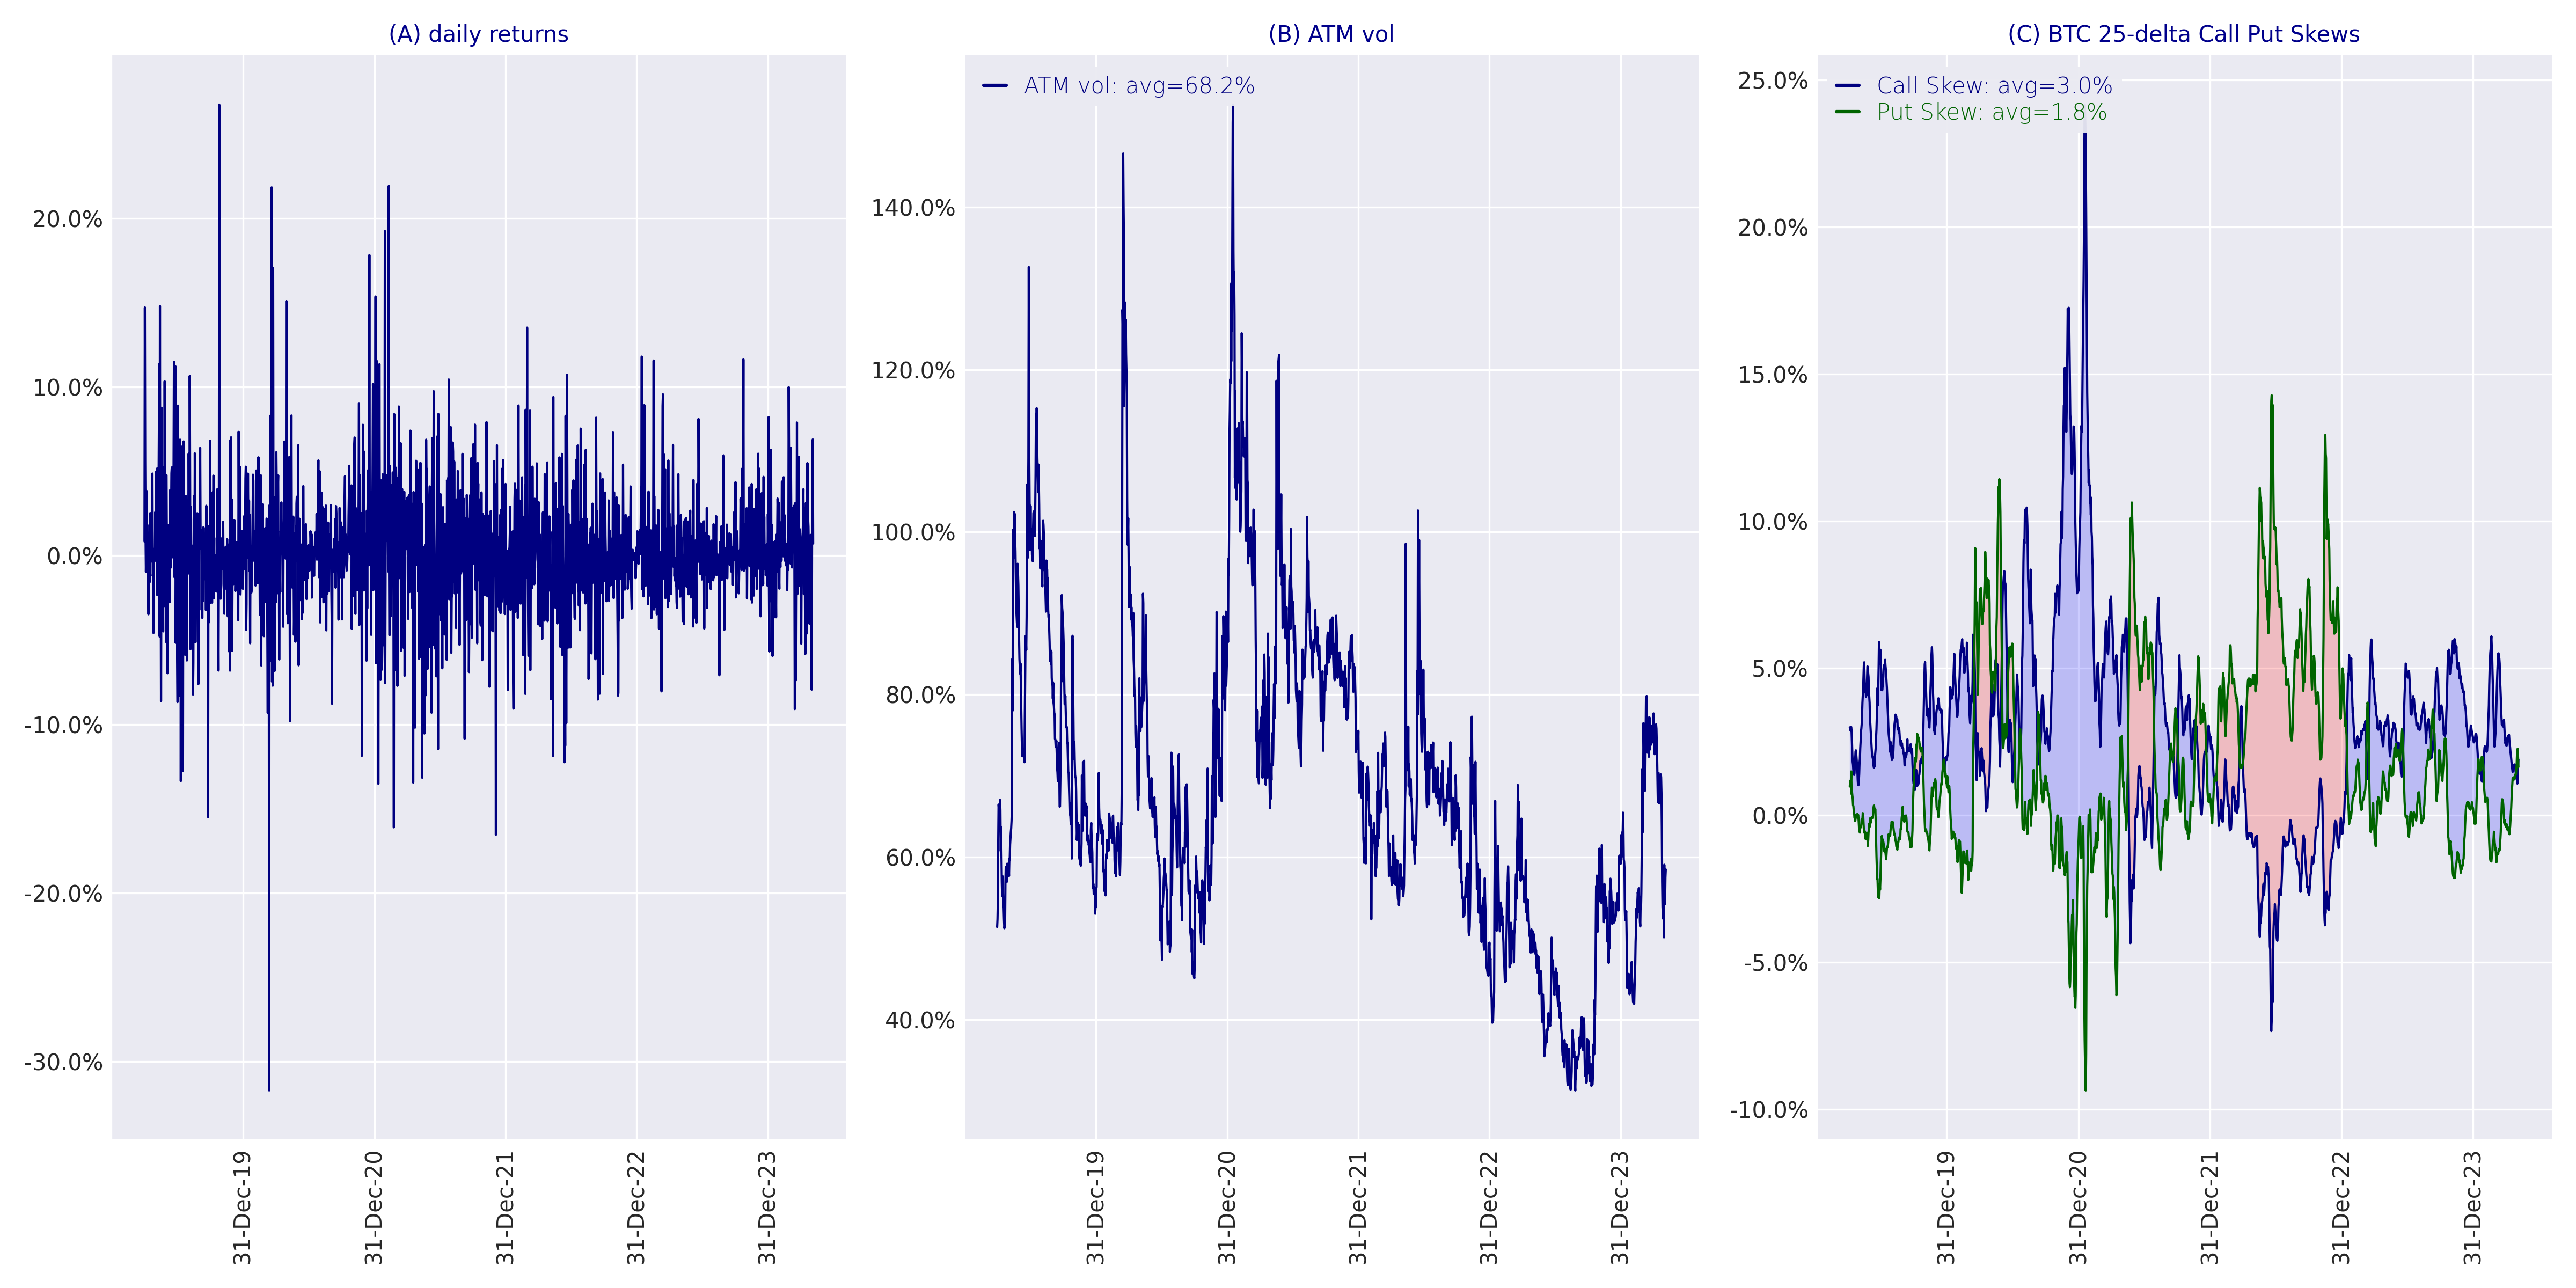
\includegraphics[width=1\linewidth]{figures/skew_risk_premias.PNG}
    \label{fig:dynamics}
\end{figure}

To account for empirical features of crypto options markets, we develop a derivatives pricing model that incorporates two Hawkes processes, one for positive and one for negative jumps.
These processes capture the clustering of jumps, driven by self- and cross-excitation, effectively capturing the structure of jump arrival times.
The model can be calibrated to the joint dynamics of BTC prices and of BTC implied volatility surfaces.
In particular, we explore the resulting positive and negative jump risk premia, defined as the difference in expected jump magnitudes between the statistical measure and the risk-neutral measures.

Importantly, our model accommodates changing market preferences for skewness risk, when investors shift their demands between put options to hedge the downside risk and call options to capture positive upside. The preference for call options with upside potential is consistent with evidence from the equity market literature indicating some investors' preferences for assets offering lottery-like payoffs, see, e.g. \cite{bali2011maxing}, \cite{thaler1988anomalies}, \cite{kumar2009gambles}. In cryptocurrency option markets, such preferences for capturing the upside manifest in inflated prices of out-of-the-money call options during bullish periods, which produces positive risk premia of positive jumps.

Furthermore, the positive implied volatility skew is also present in the market data of so-called ``meme'' stocks.
Options activity in these stocks is characterised by strong demand and high volumes for call options and by a positive spot-volatility correlation.
\cite{gupta2025} introduce the ``Equity Euphoria Indicator'', which measures the percentage of stocks with a positive implied skew ranging from $0\%$ to $100\%$.
The most recent values, 10\% as of January 2025 and 11.9\% as of September 2025, are close to the levels observed during the Dot.com bubble in late 1990 and the post-Covid rally in 2021.
We notice that implied skews on ``meme'' stocks change sign to negative during severe bear market periods, so that structurally we cannot model the dynamics of these stocks using a stochastic volatility model with a constant correlation parameter.
Adding jumps arriving at a constant intensity rate, as for the Bates model (\cite{bates1996jumps}), would not improve the structural consistency of the model dynamics, unless we specify stochastic intensity rates for positive and negative jumps.
Thus, our model represents a simple construction to model the dynamics of stocks with varying signs of implied skew.
It is straightforward to incorporate stochastic volatility in our framework; however, we skip this feature to reduce the number of model parameters.

Our work contributes to the existing literature in several areas.
First, the model of the price process allows one to identify and understand the factors that drive variations in jump risk premia, in particular, how jump intensities adapt in response to the occurrence of jumps.
Extending the work of \text{\cite{hainaut2016bivariate,Hainaut2016,hainaut2017clustered}} on Hawkes processes, we assume that the dynamics of these jump intensities are governed by a bivariate Hawkes process with cross-excitation.
Jump intensities increase with jump arrivals and decrease with time.
As such, the model accounts for changes in asset prices and option prices stemming not only from movements in the underlying price, but also from variations in jump intensities.

Second, alongside specifying the pricing model, we derive the measure change between the statistical and risk-neutral measures. We provide a rigorous treatment of the measure change underlying the model. In particular, we derive explicit conditions under which the Radon-Nikodym derivative defining the transition from the statistical to the risk-neutral measure is a true martingale. This ensures that the pricing measure is well-defined and that the model is free of arbitrage. The measure change allows us to derive the jump risk premia associated with positive and negative jumps as the difference between expected jump expected jump contributions.
A jump risk premium therefore quantifies the difference between market expectations (from options prices) and market realisations (from the price history) and can be interpreted as a measure of market sentiment. As option prices (under the risk-neutral measure) reflect expectations about future jumps and their intensities, in our setting, investors pay a risk premium for call options due to positive jumps if they are optimistic (positive skewness of option prices). Likewise, investors pay a risk premium for put options due to negative jumps if they are pessimistic (negative skewness of option prices).

We further develop an estimation and calibration procedure that takes into account both historical BTC price dynamics and options data. In the time period considered (May 2019 to October 2023), both positive and negative risk premia are observed, with frequent periods where the implied jump risk is higher than the realised jump risk. The last observation is consistent with the findings on the variance risk premia, e.g. \citep{Carr2009,Granelli2016}.

Third, the cryptocurrency market is known to have at times a large basis or cost-of-carry in its futures prices, as well as large swings in the basis.
For example, the annualised basis of one-month BTC futures on Deribit on 5 April 2021 was $35\%$, and -- after a sell-off on 19 May 2021 -- dropped to $-54\%$.
Both positive and negative carry are regularly observed in the market.
These can only partially be explained by the funding costs associated with perpetual futures.
Therefore, we investigate the relationship between the inferred jump risk premia and the carry of one-month BTC futures to determine whether risk preferences, beyond standard funding costs from perpetual contracts, significantly influence futures pricing dynamics.

Finally, the presence of jumps imposes challenges in risk management and hedging, both in terms of the magnitude of losses and in the unpredictability of jumps. Hedging strategies in crypto markets have been investigated by \citep[e.g.][]{liu2023hedging,matic2023hedging,lucicsepp2024}. Here, we investigate whether the risk premia, which capture market participants' forward-looking risk preferences, can be systematically earned through delta-hedged options trading strategies.

The Hawkes process, or self-exciting process, was introduced by \citep{Hawkes1971,Hawkes1974}, see also
\citep{Errais2010,Hawkes2018,Bacry2015,embrechts2011multivariate,hainaut2018hedging,hainaut2016bivariate} for reviews and applications of Hawkes processes in finance.
There is a vast literature on jump risk and jump risk premia, \citep[e.g.][]{bates1996jumps,bates2000post,pan2002jump,bakshi2003delta,Eraker2004,broadie2007model,santa2010crashes,christoffersen2012dynamic,nguyen2019risk}.
Skewness and their relation to risk premia are treated in \citep[e.g.][]{bakshi2003stock} with a focus on the options market, and from a behavioural perspective in \citep[e.g.]{bali2011maxing}.
The literature on risk premia in cryptocurrency markets is growing \citep[e.g.][]{alexander2021bitcoin,alexander2023delta,almeida2024risk,dobrynskaya2024downside}.

The paper is organised as follows.
 In Section \ref{sec:model}, we develop the model and derive a number of results, such as moment-generating functions and the equivalent measure change.
 Section \ref{sec:two_stage} introduces the estimation method that accompanies the model.
 In Section \ref{sec:jumps_premia}, we specify the jump risk premia.
 Section \ref{sec:results} presents the empirical results, that is, exploring the historical jump risk premia, the relationship between the jump risk premia and the futures basis, as well as the ability of the jump risk premia to forecast one-day ahead option portfolio returns that can be used to improve hedging strategies.
 All calculations in this work can be reproduced with codes available in Quantlet \href{https://github.com/QuantLet/HJP/tree/main/codes/}{
\includegraphics[height=\baselineskip]{figures/qletlogo_tr.png}}.

\section{Model specification}\label{sec:model}

\subsection{Price dynamics under $\mathbb{P}$-measure}
\label{subsec:model}
Our model extends the univariate Hawkes process dynamics considered by \cite{hainaut2018hedging}; see also \cite{hainaut2017clustered} and Chapter 4 of \cite{hainaut2022continuous} for variants of the univariate model and \cite{hainaut2016bivariate,Hainaut2016} for bivariate, more restricted models. To account for the empirical evidence of clustered positive and negative jumps, we incorporate two jump components with self-excitement and cross-excitement.

Let $\left(\Omega,\ \mathcal{F},\ \mathbb{P}\right)$ be a probability space with information filtration $\left(\mathcal{F}_t\right)$. The adapted price process $S_t$ is modeled as the sum of a continuous part driven by a Brownian motion and two jump components for positive and negative jumps, respectively. The intensities of the jump components are latent processes $\lambda^{+}_{t}$ and $\lambda^{-}_{t}$.
The arrival times of positive and negative jumps are modeled by two counting processes, abbreviated by $N^{(1)}_{t}$ and $N^{(2)}_{t}$, respectively.

We introduce the following price dynamics under the statistical $\mathbb P$ measure:
\begin{align}
  \frac{\dd S_t}{S_{t-}} &= \mu \, \dd t  + \sigma \, \dd W_t
     \label{eq:dS}\\
    &\phantom{=\,}
    + \Big((\e^{J^+}-1)\, \dd N_t^{(1)}- \lambda_t^+ \E(\e^{J^+}-1) \, \dd t \Big)
    + \Big((\e^{J^-}-1)\, \dd N_t^{(2)}- \lambda_t^- \E(\e^{J^-}-1)\,
      \dd t\Big), \nonumber \\%\label{eq:comp}\\
  \begin{pmatrix}
    \dd \lambda_t^+\\
    \dd \lambda_t^-
  \end{pmatrix}
  &=
    \begin{pmatrix}
      \kappa^+ (\theta^+-\lambda_t^+)\\
      \kappa^- (\theta^--\lambda_t^-)
    \end{pmatrix}\, \dd t %
  +
  \begin{pmatrix}
    \beta_{11} & \beta_{12}\\
    \beta_{21} & \beta_{22}
  \end{pmatrix} %
                 \begin{pmatrix}
                   J^+\, \dd N_t^{(1)}\\
                   J^-\, \dd N_t^{(2)}
                 \end{pmatrix} \label{eq:bi-Hawkes},
\end{align}
where $\mu$ is a constant drift parameter, $\sigma$ is a constant volatility parameter, $W_t$ is a standard Brownian motion, and $N^{(1)}_t$ and $N^{(2)}_t$ are counting processes for the arrival of positive and negative jumps, with stochastic intensities $\lambda^+_t$ and $\lambda^-_t$ given in Equation~\eqref{eq:bi-Hawkes}. Jump sizes $J^+$ and $J^-$ of positive and negative jumps have probability density functions (PDFs) $\varpi^+$ and $\varpi^-$, respectively, given by shifted exponential distributions specified below.
The jump parts in dynamics (\ref{eq:dS}) are adjusted by deterministic jump compensators, so the expected drift is determined by $\mu$. The coefficients $\beta_{ij}$, $i,j=1,2$, determine the level of excitement induced by jumps on the intensities.
Their signs are set by $\beta_{11}, \beta_{21}\geq0$ and $\beta_{12},
\beta_{22} \leq 0$, so that all jump realisations lead to jumps in intensity rates. We impose the following constraints on the jump parameters:
\begin{equation}
\kappa^+ > \beta_{11}\E J^+ + \beta_{12}\E J^-, \quad
\kappa^- > \beta_{21}\E J^+ + \beta_{22}\E J^-.
\label{eq:constraints}
\end{equation}
These restrictions guarantee that the expected asymptotic values of the intensities are finite,
 i.e., $\lim_{t\rightarrow \infty}\E\lambda^+_t<\infty$ and $\lim_{t\rightarrow \infty}\E\lambda^-_t<\infty$. Moreover, conditions~\eqref{eq:constraints} also guarantee that the asymptotic variances of the intensities are finite,
i.e., $\lim_{t\to\infty}\text{Var}(\lambda^+_t)<\infty$ and $\lim_{t\to\infty}\text{Var}(\lambda^-_t)<\infty$,
ensuring stationarity of the bivariate intensity process.
For details, see Appendix~\ref{sec:finite_expected_intensities}.

  For the later exposition, we explicitly state the independence of
  the Brownian motion and the jump components:
  \begin{assumption}[Independence]
    \label{assumption:independence}
The Brownian motion $W$ is independent of the marked point processes
$\big(N^{(1)},\{J^{+}_j\}\big)$ and $\big(N^{(2)},\{J^{-}_j\}\big)$, and
$\Fc=\Fc^W\vee \Fc^J$, where $\Fc^{J}$ is the natural filtration of the two marked point processes.
\end{assumption}

The solution to the dynamics in (\ref{eq:dS}) is given by:
  \begin{align}
    S_t &= S_0 \, \exp\left(\left(\mu-\frac{\sigma^2}{2}\right) t + \sigma W_t \right)\\
    &\phantom{=\,} \cdot \exp\left(
     \Big(\sum_{j=1}^{N_t^{(1)}} J_j^+ -\E(\e^{J^+}-1) \int_0^t \lambda_s^+\, \dd s\Big)
    + \Big(\sum_{j=1}^{N_t^{(2)}} J_j^- -\E(\e^{J^-}-1) \int_0^t \lambda_s^-\, \dd s\Big)
    \right),\nonumber\\
    \lambda_t^+ &= \theta^+ + \e^{-\kappa^+ t} (\lambda^+_0 - \theta^+)
                  + \beta_{11} \int_0^t \e^{-\kappa^+ (t-s)}\, J^+_s\,
                  \dd N_s^{(1)} %
                  + \beta_{12} \int_0^t \e^{-\kappa^+ (t-s)}\, J^-_s\,
                  \dd N_s^{(2)}\label{eq:lambda_p_sol},\\
    \lambda_t^- &= \theta^- + \e^{-\kappa^- t} (\lambda^-_0 - \theta^-)
                  + \beta_{21} \int_0^t \e^{-\kappa^- (t-s)}\, J^+_s\,
                  \dd N_s^{(1)} %
                  + \beta_{22} \int_0^t \e^{-\kappa^- (t-s)}\, J^-_s\,
                  \dd N_s^{(2)}\label{eq:lambda_m_sol}.
  \end{align}
We also specify the dynamics of the log return $X_t:=\ln \left(S_t/S_0\right)$ which is given by:
\begin{equation}\label{eq:dx}
\begin{split}
      \dd X_t  & = \left(\mu-\frac{\sigma^2}{2}\right) \dd t + \sigma \,\dd W_t \\
  & + \Big(J^+\, \dd N_t^{(1)} - \lambda_t^+ \E(\e^{J^+}-1) \, \dd t\Big)
  + \Big(J^-\, \dd N_t^{(2)}- \lambda_t^-\E(\e^{J^-}-1)\, \dd t\Big).
  \end{split}
\end{equation}
In summary, the model incorporates three state variables $(X_t, \lambda^+_t, \lambda^-_t)$. The model parameters include a drift $\mu$ and the volatility $\sigma$ of the continuous component;
eight parameters for the intensities of positive and negative jumps $(\kappa^{+},\ \theta^{+},\ \beta_{11},\ \beta_{12})$ and $(\kappa^{-},\ \theta^{-},\ \beta_{21},\ \beta_{22})$, respectively;
four parameters for PDFs for jumps in returns: $\varpi^{+}(j^{+})$ and $\varpi^{-}(j^{-})$, as defined next.

We assume that the sizes of positive and negative jumps are driven by shifted exponential distributions with the following PDFs:\footnote{
The shifted exponential distribution is the maximum-entropy distribution on a half-line given a known mean, making it the least informative -- and therefore most parsimonious -- choice consistent with the first moment of observed jump sizes, see e.g.\ Chapter 12 of \cite{Cover2006}. Moreover, its exponential form is essential for the analytical tractability of the Laplace transforms that underpin the affine structure of the model and the closed-form measure change.}
\begin{align}
\label{eq:jump}
\begin{split}
&\varpi^{+}(j)  = \frac{1}{\eta^{+}}\exp\left( -\frac{1}{\eta^{+}} (j-\nu^{+} )  \right) \mathbbm{1}_{\{j>\nu^{+}\}},\\
&\varpi^{-}(j)  = \frac{1}{\eta^{-}}\exp\left( \phantom{-}\frac{1}{\eta^{-}} (j-\nu^{-} )   \right) \mathbbm{1}_{\{j<\nu^{-}\}},
\end{split}
\end{align}
with $\eta^+,\eta^->0$ controlling the sizes of positive and negative jumps, respectively, and with $\nu^{+}>0$ and $\nu^{-}<0$ being thresholds.
The expected jump sizes are $\eta^+ + \nu^+$ and $-\eta^-+\nu^-$, respectively.
The Laplace transforms of the jump size distributions (extended to $\R_-$ for negative jumps) are given by
\begin{align}
  \mathcal L^{(+)}(\omega)
    &= \int_{\nu^+}^\infty e^{-\omega j}\,\varpi^+(j)\,\mathrm{d}j
     = \frac{e^{-\nu^+ \omega}}{1 + \eta^+ \omega},
    &&\quad  \Re\!\left(\frac{1}{\eta^+} + \omega\right) > 0,
    \label{eq:L_p} \\
  \mathcal L^{(-)}(\omega)
    &= \int_{-\infty}^{\nu^-} e^{-\omega j}\,\varpi^-(j)\,\mathrm{d}j
     = \frac{e^{-\nu^- \omega}}{1 - \eta^- \omega},
    &&\quad  \Re\!\left(\frac{1}{\eta^-} - \omega\right) > 0,
    \label{eq:L_m}
\end{align}
where $\omega\in \mathbb{C}$ and $\text{Re}(\cdot)$ denotes the real part of a value. Throughout, we assume $\eta^{+}<1$, so that $\E(e^{J^{+}})=\Lp(-1)<\infty$ and the jump compensators in Equation~\eqref{eq:dS} are finite; no analogous condition is needed for negative jumps, and the estimate $\widehat{\eta}^{+}=0.031$ in Table~\ref{tab:calibrated} satisfies the condition comfortably.

Jump compensators are calculated using Equations~\eqref{eq:L_p} and \eqref{eq:L_m} as follows:
  \begin{align*}
    \E\left(\e^{J^+}-1\right) &= \int_{\nu^+}^\infty \left(\e^{j}-1\right) \varpi^+(j) \dd j = \frac{\e^{\nu^+}}{1-\eta^+}-1,\\
    \E\left(\e^{J^-}-1\right) &= \int^{\nu^-}_{-\infty} \left(\e^{j}-1\right) \varpi^-(j) \dd j = \frac{\e^{\nu^-}}{1+\eta^-}-1.
  \end{align*}

We specify threshold parameters $\nu^+$ and $\nu^-$ for flexibility in defining the minimum size of jumps for empirical inference. The thresholds $\hat \nu^+$ and $\hat \nu^-$ can be estimated using a peak-over-threshold (POT) approach discussed in Section \ref{sec:firststage}.

\subsection{Moment-generating function of joint dynamics}

The moment generating function (MGF) of the log-return variable $X_t=\ln (S_t/S_0)$ and jump intensities will be used for the equivalent measure change in Section \ref{sec:Q} and for the option pricing procedure in Section \ref{sec:second_stage}. The following Proposition extends Proposition 2.2 of \cite{hainaut2018hedging} to the bivariate Hawkes process.
\begin{proposition}\label{prop:MGF}
    The MGF of joint variables $(X_T, \lambda^+_T, \lambda^-_T)$, $T\geq t$, generalised to complex arguments, is given by:
    \begin{equation}\label{eq:mgf_p}
    \begin{split}
        G^{\mathbb{P}}(\omega,\omega^+,\omega^-;t,T,X_t,\lambda_t^+, \lambda_t^-) & \equiv\E^{\mathbb{P}}\left(\exp(\omega X_T + \omega^+\lambda^+_T + \omega^-\lambda^-_T)\big|X_t, \lambda^+_t, \lambda^-_t\right)\\
        & = \exp\left(A(t,T)+ \omega X_t + C(t,T)\lambda_t^+ + D(t,T)\lambda_t^-\right),
    \end{split}
    \end{equation}
    for $\omega, \omega^+, \omega^- \in \mathbb{C}$, where the functions $A, C,\text{and } D$ solve the following non-linear system of ordinary differential equations (ODEs):
    \begin{equation*}
    \begin{split}
          \frac{\partial}{\partial t} A(t,T) &= - \mu \omega - \frac{\sigma^2}{2}\left(\omega^2-\omega\right) - \kappa^+\theta^+C(t,T) - \kappa^-\theta^-D(t,T), \\
          \frac{\partial}{\partial t} C(t,T) &= -\mathcal{L}^{(+)}(-\omega-C(t,T)\beta_{11}-D(t,T)\beta_{21}) + \kappa^+C(t,T) + \omega\Big(\frac{e^{\nu^+}}{1-\eta^+}-1\Big) + 1,\\
          \frac{\partial}{\partial t} D(t,T) &= -\mathcal{L}^{(-)}(-\omega-C(t,T)\beta_{12}-D(t,T)\beta_{22}) + \kappa^-D(t,T) + \omega\Big(\frac{e^{\nu^-}}{1+\eta^-}-1\Big) + 1,
    \end{split}
    \end{equation*}
    where $A(T,T) =0$, $C(T,T)=\omega^+$, $D(T,T)=\omega^-$ with operators $\mathcal L^+$ and $\mathcal L^-$ defined in Equations~\eqref{eq:L_p} and \eqref{eq:L_m}, respectively.
\end{proposition}
See Appendix \ref{sec:proofs} for the \hyperref[proof:prop:MGF]{proof}.

\subsection{Equivalent risk-neutral measure $\mathbb{Q}$}\label{sec:Q}

We now construct the model dynamics under an equivalent martingale measure $\mathbb{Q}$ such that the discounted stock
price process is a martingale. This is an extension of \citep{hainaut2018hedging} to a bivariate self-exciting Hawkes process.
Introduce the Radon-Nikodym derivative process defined by:
\begin{align}
  \frac{\text{d}\mathbb{Q}}{\text{d}\mathbb{P}}\Big|_{\mathcal{F}_t} = \frac{M_t}{M_0},\quad t\geq 0,
\end{align}
where $(M_t)_{t\geq 0}$ is a local martingale under $\mathbb{P}$, specified below.

Define exponential processes of the form
\begin{equation}\label{eq:RD}
\begin{split}
  M_t\left(\xi^+, \xi^-, \varphi\right) \overset{\text{def}}=
  &\exp\left\{
  q^+_1(\xi^+)\lambda^+_t + \xi^+\sum_{j=1}^{N_t^{(1)}}J^+_j
      + q^-_1(\xi^-)\lambda^-_t + \xi^-\sum_{j=1}^{N_t^{(2)}}J^-_j
  \right\} \\
  &\cdot \exp \left\{
  q_2\left(\xi^+, \xi^-\right)t
  \right\}\\
  &\cdot \exp \left\{
  -\frac{1}{2}\int_0^t \varphi^2(s)ds -
  \int_0^t \varphi(s)dW_s
  \right\},
  \end{split}
\end{equation}
where $\xi^+, \xi^- \in \mathbb{R}$ are two parameters that specify the risk premia of positive and negative jumps, respectively, and that are to be estimated from options data. $q_1^+(\xi^+), q_1^-(\xi^-), q_2(\xi^+, \xi^-)$ are  real-valued functions, and $\varphi(t)$ is a process adapted to $\{\mathcal{F}_t\}_{t\geq 0}$.
In Proposition \ref{prop:risk-neutralisation} below, we will choose
\begin{equation}
\varphi(t)=\varphi + \varphi^+\lambda_t^+ + \varphi^-\lambda_t^-,
\end{equation}
where $\varphi, \varphi^+, \varphi^-\in \R$ are constants.
We note that the process $(M_t)_{t\geq 0}$ is strictly positive, so that, provided it is a martingale, the probability measures $\mathbb P$ and $\mathbb Q$ are absolutely continuous.
The following proposition specifies martingale conditions for $(M_t)_{t\geq 0}$.

\begin{proposition}\label{prop:martingaleConditions}
If there exists a solution specified as functions $q_1^+(\xi^+)$,  $q_1^-(\xi^-)$ and $q_2(\xi^+, \xi^-)$ of the following system:
\begin{equation}\label{eq:M1}
\begin{split}
        q_1^+(\xi^+)\kappa^+\theta^+ +q_1^-(\xi^-)\kappa^-\theta^-+q_2(\xi^+, \xi^-) &=0,\\
        \mathcal L^{(+)}(-\chi^+)-1-q_1^+(\xi^+)\kappa^+ &=0,\\
        \mathcal L^{(-)} (-\chi^-)-1-q_1^-(\xi^-)\kappa^-&=0,
  \end{split}
\end{equation}
then $(M_t)_{t\geq 0}$ is a local martingale. Here, we introduce new variables $\chi^+$ and $\chi^-$ as follows:
\begin{equation}\label{eq:chi}
\begin{split}
\chi^+ & = q_1^+(\xi^+)\beta_{11} + q_1^-(\xi^-)\beta_{21}+\xi^+,\\
\chi^- & = q_1^+(\xi^+)\beta_{12} + q_1^-(\xi^-)\beta_{22}+\xi^-.
  \end{split}
\end{equation}
\end{proposition}
See Appendix \ref{sec:proofs} for the \hyperref[proof:prop:martingaleConditions]{proof}.

Proposition~\ref{prop:martingaleConditions} establishes that $M_t$, satisfying~\eqref{eq:M1}, is a positive local martingale under $\mathbb{P}$.
However, for the measure change $d\mathbb{Q}/d\mathbb{P}|_{\mathcal{F}_t} = M_t/M_0$
to define a valid probability measure, $M_t$ must be a \emph{true} martingale,
i.e., $\mathbb{E}^{\mathbb{P}}[M_t] = M_0$ for all $t \geq 0$. Since every
non-negative local martingale is a supermartingale, one always has
$\mathbb{E}^{\mathbb{P}}[M_t] \leq M_0$; it remains to rule out strict inequality.
For the concrete measure change employed in this paper, we establish martingale conditions in Proposition \ref{prop:true_mg} below.

We note that the system of equations in~(\ref{eq:M1}) is non-linear because of its variables entering into non-linear functions $\mathcal L^{(+)}$ and $\mathcal L^{(-)}$. First, we make the following canonical assumption that the risk premium functions are linear.
\begin{assumption}
We assume that the real-valued functions are specified by means of a linear system of equations as follows:
\begin{equation}\label{eq:c}
\begin{split}
    q_1^+(\xi^+)      &= c^++\xi^+\\
    q_1^-(\xi^-)      &= c^-+\xi^-\\
    q_2(\xi^+, \xi^-) &= c+\xi^++\xi^-,
  \end{split}
\end{equation}
where $c^+, c^-, c \in \mathbb{R}$ are internal parameters which are determined so that the system in Equation~\eqref{eq:M1} is satisfied for any choice of $\xi^+$ and $\xi^-$.
\end{assumption}

Equation \eqref{eq:c} preserves the model structure under $\mathbb{Q}$, so $\mathbb{P}$- and $\mathbb{Q}$-parameters are comparable one-to-one and the jump risk premia $\gamma^{\pm}$ are well defined as compensator differences. Second, we linearise the system of equations \eqref{eq:M1}, by making the following assumption.

\begin{assumption}
The variables $\chi^+$ and $\chi^-$ in~\eqref{eq:chi} are external variables that specify the risk premium, while variables $\xi^+$ and $\xi^-$ become internal parameters inferred using Equation~\eqref{eq:chi}.
\end{assumption}

\begin{corollary}
  \label{cor:spec}
The specification of the risk premium is defined by the two external parameters $\chi^+$ and $\chi^-$.
The internal parameters of linear risk premium functions in~\eqref{eq:c}, internal risk premia $\xi^+$ and $\xi^-$ parameters in~\eqref{eq:chi} along the martingale conditions in Equation~\eqref{eq:M1} are determined by five internal parameters $(\xi^+, \xi^-, c^+, c^-, c)$ which are obtained by solving the following linear system:
    \begin{equation}\label{eq:system}
        \begin{pmatrix}
        1+\beta_{11} &   \beta_{21} & \beta_{11} & \beta_{21} & 0\\
        \beta_{12} & 1+\beta_{22} & \beta_{12} & \beta_{22} & 0\\
        1+\kappa^+\theta^+ & 1+\kappa^-\theta^- & \kappa^+\theta^+ & \kappa^-\theta^- & 1\\
        1&0&1&0&0\\
        0&1&0&1&0
        \end{pmatrix}  \begin{pmatrix}\xi^+\\ \xi^-\\ c^+\\ c^-\\ c \end{pmatrix} =
        \begin{pmatrix}
        \chi^+ \\ \chi^- \\ 0 \\ \left(\mathcal{L}^{(+)}(-\chi^+)-1\right)\big/ \kappa^+\\ \left(\mathcal{L}^{(-)}(-\chi^-)-1\right)\big/ \kappa^-
        \end{pmatrix}.
    \end{equation}
\end{corollary}

\begin{proposition}\label{lemma:solution}
    The system of linear equations in~\eqref{eq:system} in $(\xi^+, \xi^-, c^+, c^-, c)$ has a unique solution.
\end{proposition}
\begin{proof}
The determinant of the coefficient matrix in Equation~\eqref{eq:system} is equal to one, so the matrix is invertible and a solution to the linear system exists and is unique.
\end{proof}

This chain of results establishes that the equivalent martingale
measure $\mathbb{Q}$ is fully characterised by the two external risk
premium parameters $\chi^+$ and $\chi^-$, which can be interpreted as
market-implied jump risk premia for positive and negative jumps,
respectively. Given any such pair $(\chi^+, \chi^-)$, the
corresponding internal parameters $(\xi^+, \xi^-, c^+, c^-, c)$ that
define the Radon-Nikodym derivative are uniquely determined by solving
the linear system in Equation~\eqref{eq:system}. For any pair
  $(\chi^{+},\chi^{-})$ satisfying the
  admissibility condition (C1) below, this construction yields a
  strictly positive \emph{local} martingale $(M_t)_{t\ge0}$. Its true
  martingale property --- and hence the well-posedness of the measure
  change --- is established under conditions (C1) and (C3) in
  Proposition~\ref{prop:true_mg}, and verified for all calibrated
  parameter sets in Section \ref{sec:verif}.

Crucially, the transformation of the model from the physical measure $\mathbb{P}$ to the risk-neutral measure $\mathbb{Q}$ depends only on the values of $\chi^+$ and $\chi^-$. This leads to a clean and tractable separation between the statistical and risk-neutral dynamics, which then enables model calibration and risk premium estimation from observed option prices. As shown in Proposition~\ref{prop:HawkesUnderQ}, the jump intensity dynamics under $\mathbb{Q}$ inherit a similar structure to those under $\mathbb{P}$, with appropriately adjusted parameters. Thus, the model maintains internal consistency and interpretability under both measures, while enabling flexible inference of jump risk premia from market data.

\begin{proposition}[Jump intensity dynamics under the risk-neutral measure $\q$ ]\label{prop:HawkesUnderQ}  %
    Let
    $N^{(1),\mathbb{Q}}_t$ and $N^{(2),\mathbb{Q}}_t$ be the counting processes of positive and negative jumps under the measure $\mathbb{Q}$ with intensities
    \begin{equation}
        \lambda^{+,\mathbb{Q}}_t=\mathcal{L}^{(+)}\left(-\chi^+\right) \lambda^+_t,\qquad
        \lambda^{-,\mathbb{Q}}_t=\mathcal{L}^{(-)}\left(-\chi^-\right) \lambda^-_t,
    \end{equation}
    where $\chi^+$ and $\chi^-$ are external risk premium parameters in Eq.\eqref{eq:chi} satisfying
  $1 - \eta^+ \chi^+>0$ and $1 + \eta^-\chi^->0$.

The evolution of jump intensity rates  $\lambda^{+,\mathbb{Q}}_t$ and $\lambda^{-,\mathbb{Q}}_t$ under $\mathbb{Q}$ are driven by the following dynamics:
    \begin{equation}\label{eq:dxi}
\begin{split}
   \dd \lambda^{+,\mathbb{Q}}_t &= \kappa^+ \left(\theta^{+, \mathbb{Q}}-\lambda^{+,\mathbb{Q}}_t\right)\dd t
         + \beta^{\mathbb{Q}}_{11} J^{+, \mathbb{Q}}\, \dd N^{(1),\mathbb{Q}}_t
         + \beta^{ \mathbb{Q}}_{12} J^{-, \mathbb{Q}}\, \dd N^{(2),\mathbb{Q}}_t\\
   \dd \lambda^{-,\mathbb{Q}}_t &= \kappa^- \left(\theta^{-, \mathbb{Q}}-\lambda^{-,\mathbb{Q}}_t\right)\dd t
         + \beta^{\mathbb{Q}}_{21} J^{+, \mathbb{Q}} \,\dd N^{(1),\mathbb{Q}}_t
         + \beta^{\mathbb{Q}}_{22} J^{-, \mathbb{Q}} \,\dd N^{(2),\mathbb{Q}}_t,
\end{split}
\end{equation}
    where
    \begin{align}
         \theta^{+, \mathbb{Q}} &= \mathcal{L}^{(+)}(-\chi^+)\theta^+,\
         \beta^{\mathbb{Q}}_{11} = \mathcal{L}^{(+)}(-\chi^+)\beta_{11},\
         \beta^{\mathbb{Q}}_{12} = \mathcal{L}^{(+)}(-\chi^+)\beta_{12},\\
         \theta^{-,\mathbb{Q}} &= \mathcal{L}^{(-)}(-\chi^-)\theta^-,\
         \beta^{\mathbb{Q}}_{21} = \mathcal{L}^{(-)}(-\chi^-)\beta_{21},\
         \beta^{\mathbb{Q}}_{22} = \mathcal{L}^{(-)}(-\chi^-)\beta_{22},
    \end{align}
    Here, $J^{+, \mathbb{Q}}$ and  $J^{-, \mathbb{Q}}$ are realizations of positive and negative jumps from distributions with probability density functions(PDFs)
    $\varpi^{+, \mathbb{Q}}(j^+)$ and $\varpi^{-, \mathbb{Q}}(j^-)$:
    \begin{align*}
        \varpi^{+,\mathbb{Q}}(j) &= \frac{1}{\eta^{+, \mathbb{Q}}}\exp\left(-\frac{1}{\eta^{+, \mathbb{Q}}}(j-\nu^+)\right)\mathbbm{1}_{\{j > \nu^+\}},\\
        \varpi^{-,\mathbb{Q}}(j) &= \frac{1}{\eta^{-, \mathbb{Q}}}\exp\left(\phantom{-}\frac{1}{\eta^{-, \mathbb{Q}}}(j-\nu^-)\right)\mathbbm{1}_{\{j < \nu^-\}}
    \end{align*}
    where
    \begin{align}
        \eta^{+,\mathbb{Q}}
        &= \frac{\eta^+}{1-\eta^+\chi^+},\
        \eta^{-,\mathbb{Q}}
        = \frac{\eta^-}{1+\eta^-\chi^-}.
    \end{align}
\end{proposition}
See Appendix \ref{sec:proofs} for the \hyperref[proof:HawkesUnderQ]{proof}.
Proposition \ref{prop:HawkesUnderQ} indicates that the dynamics of the intensities and the PDFs of the jump sizes are specified by the two external parameters $\chi^+$ and $\chi^-$. Accordingly, for model calibration to implied volatility data, we need to infer a pair of values of $\chi^+$ and $\chi^-$ that provides the best fit.
The following proposition specifies $\varphi(t)$ such that an equivalent risk-neutral measure is obtained.
\begin{proposition}\label{prop:risk-neutralisation}
    We introduce the adapted process $\varphi(t)$ as follows:
    \begin{align}
      \label{eq:varphi2}
      \varphi(t)
      &= \frac{\mu - r}{\sigma}
      - \frac{ \E(e^{J^+}-1)
      - \mathcal{L}^{(+)}(-\chi^+)  \E^\mathbb{Q}(e^{J^{+,\q}}-1)}
        {\sigma}\, \lambda_t^+ \\
      &\phantom{=\,}
        - \frac{   \E(e^{J^-}-1)
        -\mathcal{L}^{(-)}(-\chi^-) \E^\mathbb{Q}(e^{J^{-,\q}}-1)
        } {\sigma }\lambda_t^-,\nonumber%
        \\[5pt]
      &= \frac{\mu - r}{\sigma} %
        - \frac{
        \lambda^{+}_t \E(e^{J^+}-1)
        - \lambda^{+,\mathbb{Q}}_t \E^\mathbb{Q}(e^{J^{+,\q}}-1)
        } {\sigma} %
        - \frac{
        \lambda^{-}_t \E(e^{J^-}-1)
        - \lambda^{-,\mathbb{Q}}_t \E^\mathbb{Q}(e^{J^{-,\q}}-1)
        } {\sigma },\nonumber
    \end{align}
    where $r$ is the risk free rate. Then the log return process $X_t=\ln (S_t/S_0)$ is driven under $\mathbb{Q}$ by:
    \begin{multline}
      \dd X_t   = \left(r-\frac{\sigma^2}{2}\right) \dd t + \sigma \,\dd W^{\mathbb{Q}}_t \\
       + \Big(J^{+, \mathbb{Q}}\, \dd N_t^{\mathbb{Q}, (1)} - \lambda_t^{+, \mathbb{Q}} \E^\mathbb{Q}(\e^{J^{+, \mathbb{Q}}}-1) \, \dd t\Big)
  + \Big(J^{-, \mathbb{Q}}\, \dd N_t^{\mathbb{Q}, (2)}- \lambda_t^{-, \mathbb{Q}}\E^\mathbb{Q}(\e^{J^{-, \mathbb{Q}}}-1)\, \dd t\Big), \label{eq:dxq}
  \end{multline}
    where $W^{\mathbb{Q}}$ is a standard Brownian motion under $\mathbb{Q}$, and the discounted price process is a $\mathbb Q$-martingale.
\end{proposition}
See Appendix \ref{sec:proofs} for the \hyperref[proof:prop:risk-neutralisation]{proof}.
The function $\varphi(t)$ specifies the risk premia associated with the continuous component of the process. We will discuss the jump risk premia in Section \ref{sec:jumps_premia}.

\begin{corollary}[MGF in Proposition \ref{prop:MGF} under $\mathbb{Q}$] \label{prop:MGF_q}
    The MGF of log-return $X_T$ with the dynamics in Equation~\eqref{eq:dxq} under $\mathbb{Q}$ is given by:
    \begin{equation}\label{eq:mgf_q}
    \begin{split}
        G^{\mathbb{Q}}(\omega;T,x,\lambda^{+, \mathbb{Q}}, \lambda^{-, \mathbb{Q}}) & \equiv\E^{\mathbb{Q}}\left(\exp(\omega X_T)\big|X_t, \lambda^{+, \mathbb{Q}}_t, \lambda^{-, \mathbb{Q}}_t\right)\\
        & = \exp\left(A(t,T)+ \omega X_t + C(t,T)\lambda_t^{+, \mathbb{Q}} + D(t,T)\lambda_t^{-, \mathbb{Q}}\right)\\
        & =: \exp\left(\omega X_t \right)\Ec\big(t,T;\omega;\lQp_t,\lQm_t\big), %
    \end{split}
    \end{equation}
    where functions $A, C,\text{and } D$ solve Equation~\eqref{eq:mgf_p} with $\omega^+=0, \ \omega^-=0$ and with the following substitution of model parameters:
\begin{equation}\label{eq:mgf_q1}
\begin{split}
& \mu \rightarrow r,\\
& \theta^{+} \rightarrow  \theta^{+, \mathbb{Q}} = \mathcal{L}^{(+)}(-\chi^+)\theta^+, \ \beta_{11} \rightarrow \beta^{\mathbb{Q}}_{11} = \mathcal{L}^{(+)}(-\chi^+)\beta_{11},\ \beta_{12}\rightarrow \beta^{\mathbb{Q}}_{12} = \mathcal{L}^{(+)}(-\chi^+)\beta_{12},\\
& \theta^{-} \rightarrow \theta^{-,\mathbb{Q}} = \mathcal{L}^{(-)}(-\chi^-)\theta^-, \  \beta_{21}\rightarrow \beta^{\mathbb{Q}}_{21} = \mathcal{L}^{(-)}(-\chi^-)\beta_{21}, \ \beta_{22} \rightarrow \beta^{\mathbb{Q}}_{22} = \mathcal{L}^{(-)}(-\chi^-)\beta_{22},\\
& \eta^{+} \rightarrow  \eta^{+,\mathbb{Q}} =  \frac{\eta^+}{1-\eta^+\chi^+},\ \eta^{-}\rightarrow \eta^{-,\mathbb{Q}}   = \frac{\eta^-}{1+\eta^-\chi^-}.
\end{split}
\end{equation}
\end{corollary}

 {

We state three conditions on the risk-premium pair $(\chi^{+},\chi^{-})$ for the measure change and the dynamics under $\mathbb Q$:

\begin{itemize}[leftmargin=3em,itemsep=2pt]
\item[\textup{(C1)}] \emph{Admissibility:} $1-\eta^{+}\chi^{+}>0$ and $1+\eta^{-}\chi^{-}>0$, so that
$\Lp(-\chi^{+}),\Lm(-\chi^{-})\in(0,\infty)$ and $\eta^{+,\q},\eta^{-,\q}\in(0,\infty)$.
\item[\textup{(C2)}] \emph{Stationarity under $\q$:}
 $s(\Phi^{\q}) < 0$, where
    $s(\Phi^{\q}) := \max\{\operatorname{Re}(z) : z \text{ an eigenvalue of } \Phi^{\q}\}$
is the spectral abscissa of
\begin{equation*}
\Phi^{\q} = \begin{pmatrix} -\kappa^+ + \beta^{\q}_{11}\E^\q J^{+,\q} & \beta^{\q}_{12}\E^\q J^{-,\q} \\[2pt] \beta^{\q}_{21}\E^\q J^{+,\q} & -\kappa^- + \beta^{\q}_{22}\E^\q J^{-,\q} \end{pmatrix},
\end{equation*}
where $\E^\q J^{+,\q} = \nu^+ + \eta^{+,\q}$ and $\E^\q J^{-,\q} = \nu^- - \eta^{-,\q}$.
By the Gershgorin circle theorem (as in Appendix~\ref{sec:finite_expected_intensities}), the row bounds
\begin{equation*}
\kappa^+ > \beta^{\q}_{11}\E^\q J^{+,\q} + \beta^{\q}_{12}\E^\q J^{-,\q}, \qquad \kappa^- > \beta^{\q}_{21}\E^\q J^{+,\q} + \beta^{\q}_{22}\E^\q J^{-,\q},
\end{equation*}
the direct $\q$-analogues of (\ref{eq:constraints}), are sufficient, but not necessary, for (C2).
\item[\textup{(C3)}] \emph{Non-explosion of the $R^{*}$-system:}
the $\q$-Riccati ODEs of Corollary~\ref{prop:MGF_q} with $\omega=\omega^{+}=\omega^{-}=0$ admit only the trivial solution on $[0,T]$; equivalently, the generalized Riccati system~\eqref{eq:Rstar} of Lemma~\ref{lemma:3}, with initial condition $g(0)=0$, admits $g\equiv0$ as its unique $\R^{2}_{-}$-valued solution on $[0,T]$.\\
\end{itemize}
Condition (C1) is the admissibility requirement under which the density process and the $\q$-dynamics are well defined.
Condition (C2) is the sharp $\q$-counterpart of the stationarity restriction in Equation~\eqref{eq:constraints} and matters only for longer-dated claims.
Condition (C3) is precisely the criterion of Theorem 4.4 and Remark 4.5(i)–(ii) of \cite{Mayerhofer2011}, which characterize exactly when the (ordinary or stochastic) exponential of a process already known to be a local martingale is in fact a true martingale, namely if and only if the associated transformed affine process is conservative.

\begin{proposition}
  \label{prop:true_mg}
  Let Assumption~\ref{assumption:independence} hold and let $(\chi^{+},\chi^{-})$ satisfy \textup{(C1)}. Then the density process $(M_t)_{t\ge0}$ of Eq.~\eqref{eq:RD} is a true martingale on $[0,T]$, for every finite $T>0$, if and only if condition \textup{(C3)} holds on $[0,T]$. In particular, under \textup{(C1)} and \textup{(C3)}, the measure $\q$ defined by $d\q/d\p|_{\Fc_T}=M_T/M_0$ is a probability measure equivalent to $\p$, and the risk-neutral dynamics of Propositions~\ref{prop:HawkesUnderQ} and~\ref{prop:risk-neutralisation} are well defined. Moreover, for the shifted-exponential jump sizes of Section~\ref{subsec:model}, \textup{(C1)} implies \textup{(C3)} (Remark~\ref{remark:6.3}), so $M$ is a true martingale on every finite horizon whenever \textup{(C1)} holds.
\end{proposition}

Conditions (C1) and (C2) are explicit algebraic constraints on the model and risk-premium parameters, verifiable analytically. Condition (C3) is the sharp criterion. The proof in Appendix~\ref{app:true_mg} factorises $M=M^{J}M^{W}$ into pure-jump and Brownian components and removes the Brownian factor by conditioning. By Theorem~4.4 of \cite{Mayerhofer2011}, with their Remark~4.5(i)--(ii) for the ordinary exponential of an affine functional, the pure-jump factor $M^{J}$ is a true martingale on $[0,T]$ if and only if the associated transformed affine process is conservative on $[0,T]$. This conservativeness is exactly the uniqueness of the trivial $R^{*}$-Riccati solution in (C3). In our finite-activity setting, (C1) already implies (C3) (Remark~\ref{remark:6.3}), and we report the diagnostics in Section~\ref{sec:verif}.
}

Finally, we comment on the computation of option prices:
\begin{proposition}
\label{prop:option_pricing}
Using the Lewis-Lipton formula (\cite{Lewis2001}, \cite{Lipton2002}), the value of a call option, denoted by $U^{call}$, and a put option, denoted by $U^{put}$, with strike price $K$ and maturity time $T$ is computed for log-price dynamics in Equation~\eqref{eq:dxq} under the risk-neutral measure $\mathbb{Q}$ by:
\begin{equation} \label{eq:opt1}
\begin{split}
  & U^{call}(\tau, S,K)  = e^{-r\tau}S- U(\tau, X, K), \\
	& U^{put}(\tau, S,K)  = e^{-r\tau} K - U(\tau, X, K),
\end{split}
\end{equation}
where $\tau=T-t$. Here and below, $S$ denotes the $T$-maturity forward price of the underlying (Deribit options are written on futures), so that Equations~\eqref{eq:opt1} satisfy the put--call parity $U^{call}-U^{put}=e^{-r\tau}(S-K)$; this is also the convention of the reference implementation referenced below. Here, $U(\tau, X, K)$ is the price of the capped payoff $\min(S,K)$ which is computed by:
\begin{equation} \label{eq:opt2}
\begin{split}
  U(\tau, X, K)&  = \frac{e^{-r\tau} K}{\pi} \Re\left[\int^{\infty}_{0} e^{-(iy-1/2) X^{*}}  \frac{1}{y^{2}+1/4} \Ec(\tau; \omega=iy-1/2)dy\right],
\end{split}
\end{equation}
where $X^{*}=\ln(S/K)$ is log-moneyness, $\Re(x)$ is the real part of
$x$, and
$\Ec(\tau;\omega):=\Ec\big(t,t+\tau;\omega;\lQp_t,\lQm_t\big)$
  is specified in Equation~\eqref{eq:mgf_q}  and where
    $A,C,D$ depend on $(t,T)$ only through $\tau=T-t$.
\end{proposition}
For the proof, see the proof of Proposition 5.1. in \cite{sepprakhmonov2023}.

For numerical implementation, the system of ODEs in Equation~\eqref{eq:mgf_p} must be solved numerically using standard Runge-Kutta methods. Given that the computation of the MGF part $\Ec(\tau;\omega)$ does not depend on the strike price of the option, the function $\Ec(\tau;\omega)$ can be computed on a grid and applied to the numerical calculation of call and put options at the same maturity time with different strike prices\footnote{Github project StochVolModels provides Python code with prototype implementation of option valuation using Equations~\eqref{eq:opt1} and \eqref{eq:opt2}, see \url{https://github.com/ArturSepp/StochVolModels/blob/main/stochvolmodels/pricers/hawkes_jd_pricer.py}.}.

The computational cost of the model is moderate.
For each maturity, the pricing step requires solving the two-dimensional
ODE system for $(C,D)$ via a standard fourth-order Runge-Kutta method
on a grid of the transform variable $\omega$.
Since the MGF component $\Ec(\tau;\omega)$ in Equation~\eqref{eq:mgf_q}
is independent of the strike price, it is evaluated once per maturity
and reused across all strikes in the Lewis-Lipton integration~\eqref{eq:opt2}.
The main computational cost therefore lies in the calibration optimiser,
which solves for $(\sigma, \chi^+, \chi^-)$ per maturity slice.
Using the prototype Python implementation with numba acceleration
referenced above, calibrating four implied-volatility slices
takes approximately 100 seconds on a standard desktop.
The code repository includes a ready-to-run calibration test case
for reproducing this benchmark.
For production or real-time use, warm-starting the optimiser
from the previous calibration and porting the ODE solver
to a compiled language would reduce this by at least an order of magnitude.

\section{Two stage approach calibration of the model}\label{sec:two_stage}
We adopt the following two-stage calibration approach. First, we estimate the model parameters under the statistical measure $\mathbb{P}$ from historical price data. Then, we infer the risk premia and the model parameters under the risk-neutral measure $\mathbb{Q}$ using the options data.

\subsection{Time series estimation}\label{sec:firststage}
To filter out jumps from time series of returns, we implement a POT procedure similarly to the approach in \cite{embrechts2011multivariate} and \cite[Chapter 4]{hainaut2022continuous}. We consider a sample of equally-spaced log-returns observed in the time window $[0,\ T]$.
 The POT procedure labels the log-returns that exceed the threshold as jumps. The underlying assumption is that the continuous part of the price process has normally distributed log-returns which implies that sampled returns, filtered by excluding jumps, have zero skewness and zero excess kurtosis.

Let $(X^{(\nu^+,\nu^-)}):=\left\{X_t: \nu^- < X_t < \nu^+\right\}$ the set of log-returns bounded by $\nu^-$ and $\nu^+$.
 The estimate of the thresholds is then given by:
 \begin{align}
  \left(\widehat\nu^+,\ \widehat\nu^-\right) = \underset{\nu^+, \nu^-}{\text{argmin}}  \left[
    |\text{skew}(X^{(\nu^+,\nu^-)})|+|\text{kurt}(X^{(\nu^+,\nu^-)})|
    \right],  \end{align}
 where $\text{skew}(X) = |X|^{-1}\sum_{x \in X}(x-\hat \mu_X)^3/\hat \sigma_X^3$,
       $\text{kurt}(X) = |X|^{-1}\sum_{x \in X}(x-\hat \mu_X)^4/\hat \sigma_X^4 - 3$,
      $\hat \mu_X$ and $\hat \sigma_X$ are the sample mean and standard deviation, respectively, and $|X|^{-1}$ is the sample size.
Given estimated thresholds, we identify the set of positive jump events $\mathcal{J}^+$ and the set of negative jump events $\mathcal{J}^-$ respectively as follows:\footnote{
    If the drift rate $\mu$ could be estimated accurately, one would subtract the daily expected return from the observed jump sizes. However, as estimates of $\mu$ are inherently noisy and unreliable \citep[e.g.][]{Merton1980,Jorion1999,AitSahalia1996}, and further the magnitude relative to expected jump sizes turns out to comparatively small, we set the estimate of $\mu$ to zero. Likewise, if a jump is detected during $\Delta s$, we set the diffusion part to its expectation, i.e., $\Delta W_s=0$.
}
\begin{equation}
    \begin{split}
    \mathcal{J}^+ &= \left\{J^+(s)\right\}_{s \leq T} = \left\{
      X_s \in X: X_s \geq \widehat\nu^+ \text{ and } s \leq T
      \right\},\\
      \mathcal{J}^- &= \left\{J^-(s)\right\}_{s \leq T} = \left\{
        X_s \in X: X_s \leq \widehat\nu^- \text{ and } s \leq T
        \right\}.
    \end{split}
\end{equation}

We construct the counting processes for positive jumps and for the negative jumps as follows:
\begin{equation}
    \begin{split}
    \widehat{N^{(1)}} &= \#\left\{
        X_s \in X: X_s \geq \widehat\nu^+ \text{ and } s \leq T
        \right\}, \\
    \widehat{N^{(2)}} &= \#\left\{
        X_s \in X: X_s \leq \widehat\nu^- \text{ and } s \leq T
        \right\}.
    \end{split}
\end{equation}

We denote the corresponding sequences of arrival times of positive jumps $\mathcal{T}^+$, of negative jumps $\mathcal{T}^-$, and an ordered union of jump arrival times $\mathcal{T}^{\pm}$ by:
\begin{equation}
    \begin{split}
& \mathcal{T}^+ = \left\{t \in [0,\ T]: X_t \geq \hat \nu^+ \right\} = \left\{T^+_{[1]},\ T^+_{[2]},\ ...,\ T^+_{\widehat{[N^{(1)}]}}\right\},\\
& \mathcal{T}^- = \left\{t \in [0,\ T]: X_t \leq \hat \nu^- \right\} = \left\{T^-_{[1]},\ T^-_{[2]},\ ...,\ T^-_{\widehat{[N^{(2)}]}}\right\},\\
& \mathcal{T}^{\pm} = \left\{T^{\pm}_{[1]},\ T^{\pm}_{[2]},\ ...,\ T^{\pm}_{[\widehat{N^{(1)}}+\widehat{N^{(2)}}]}\right\}.
    \end{split}
\end{equation}

Jumps sizes are independent of other random variables and follow shifted exponential distributions.
Therefore, given the shift parameter estimates $\widehat \nu^+$ and $\widehat \nu^-$ from the POT procedure, the estimators of $\eta^+$ and $\eta^-$ are given by averaging:
\begin{equation}\label{eq:mean_p_jumps_sizes}
    \begin{split}
\widehat \eta^+ &= \widehat{N^{(1)}}^{-1} \sum_{j \in \mathcal{J}^+}\left(j - \widehat \nu^+\right),\\
\widehat \eta^- &= -\widehat{N^{(2)}}^{-1} \sum_{j \in \mathcal{J}^-}\left(j + \widehat \nu^-\right).
    \end{split}
\end{equation}

Next, we estimate the parameters of the intensities dynamics via the maximum likelihood estimator (MLE). We deploy a version of the multivariate log-likelihood function documented in \cite{embrechts2011multivariate} as follows:
 \begin{align}
  \ln L' &= \sum_{T^+ \in \mathcal{T}^+} \ln \lambda^+(T^+-)\varpi^+(J^+(T^+))
          + \sum_{T^- \in \mathcal{T}^-} \ln \lambda^-(T^--)\varpi^-(J^-(T^-)) \nonumber\\
  &- \int_0^T \lambda^+(t-)\text{d}t
  - \int_0^T \lambda^-(t-)\text{d}t. %
 \end{align}
We note that the likelihood takes the left-continuous version (indicated by $T-$) of the intensities processes (see \citep[p. 232]{daley2003introduction}). Since distributions of jump sizes are already estimated throughout the POT procedure using Equation~\eqref{eq:mean_p_jumps_sizes}, we only need a partial likelihood for the intensity processes defined by:
\begin{align}
  \ln L = \sum_{T^+ \in \mathcal{T}^+} \ln \lambda^+(T^+-)
  +
   \sum_{T^- \in \mathcal{T}^-} \ln \lambda^-(T^--)
  - \int_0^T \lambda^+(t-)\text{d}t
  - \int_0^T \lambda^-(t-)\text{d}t. \label{eq:likelihood}
 \end{align}
The relationship between the intensities and the model parameters is specified for $s \in [T_{[k-1]}^\pm,\ T_{[k]}^\pm)$ and $k \in \left\{1,2,...,\ \widehat{N^{(1)}}+\widehat{N^{(2)}}\right\}$ as follows:
 \begin{align}
  \lambda^+(s) &= \theta^+ + e^{-\kappa^+\left(s - T_{[k-1]}^\pm\right)}\left(\lambda^+(T_{[k-1]}^\pm)-\theta^+\right),\\
  \lambda^-(s) &= \theta^- + e^{-\kappa^-\left(s - T_{[k-1]}^\pm\right)}\left(\lambda^-(T_{[k-1]}^\pm)-\theta^-\right).
 \end{align}

In the event of positive jump $T^+ \in \mathcal{T}^+$, the intensities jump by:
\begin{equation}
    \begin{split}
  \lambda^+(T^+) &= \lambda^+(T^+-) + \beta_{11}J^+(T^+),\\
  \lambda^-(T^+) &= \lambda^-(T^+-) + \beta_{21}J^+(T^+).
    \end{split}
\end{equation}

In the event of a negative jump $T^- \in \mathcal{T}^-$, the intensities jump by:
\begin{equation}
    \begin{split}
  \lambda^+(T^-) &= \lambda^+(T^--) + \beta_{12}J^-(T^-),\\
  \lambda^-(T^-) &= \lambda^-(T^--) + \beta_{22}J^-(T^-).
    \end{split}
\end{equation}

The integrals of the intensities in the partial likelihood Equation~\eqref{eq:likelihood} can be computed as follows:
\begin{equation}
    \begin{split}
  \int_0^T\lambda^+(t-)\text{d}t &= \sum_{k=1}^{\widehat{N^{(1)}} + \widehat{N^{(2)}}} \int_{T^{\pm}_{[k-1]}}^{T^\pm_{[k]}}\lambda^+(t-)\text{d}t\\
  &= \sum_{k=1}^{\widehat{N^{(1)}} + \widehat{N^{(2)}}}
 \theta^+(T_{[k]}^\pm-T_{[k-1]}^\pm)
 +\left(\lambda^+(T_{[k]}^\pm-)-\theta^+\right)\frac{1-e^{-\kappa^+(T_{[k]}^\pm - T_{[k-1]}^\pm)}}{\kappa^+},\\
 \int_0^T\lambda^-(t-)\text{d}t&= \sum_{k=1}^{\widehat{N^{(1)}} + \widehat{N^{(2)}}}
\theta^-(T_{[k]}^\pm-T_{[k-1]}^\pm)
+\left(\lambda^-(T_{[k]}^\pm-)-\theta^-\right)\frac{1-e^{-\kappa^-(T_{[k]}^\pm - T_{[k-1]}^\pm)}}{\kappa^-}.
    \end{split}
\end{equation}

Therefore, given a set of model parameters, the intensities and their integrals can be computed quickly in a recursive way starting from time 0. We refer to Section 5.2 of \cite{laub2021elements} and references therein for the method of directly computing the likelihood.
  We apply a numerical optimiser to obtain estimates of the jump parameters, $\hat \kappa^\pm, \ \hat\theta^\pm, \{\hat \beta_{ij}\}_{i,j=1,2}$, that maximise the likelihood.
Figure \ref{fig:empirical?intensities} illustrates the estimation procedure applied to BTC daily returns from 2019-05-30 to 2023-10-04. Table \ref{tab:calibrated} shows the parameters calibrated under the measure $\mathbb P$.

\begin{figure}
    \centering
    \caption{Subplot (A) shows BTC daily returns which are classified using the POT procedure as positive jumps (green), negative jumps (red), or non-jumps (yellow). Subplot (B) displays the model intensities estimated via MLE, calibrated using the interarrival times and magnitudes of the jumps identified by POT.}
    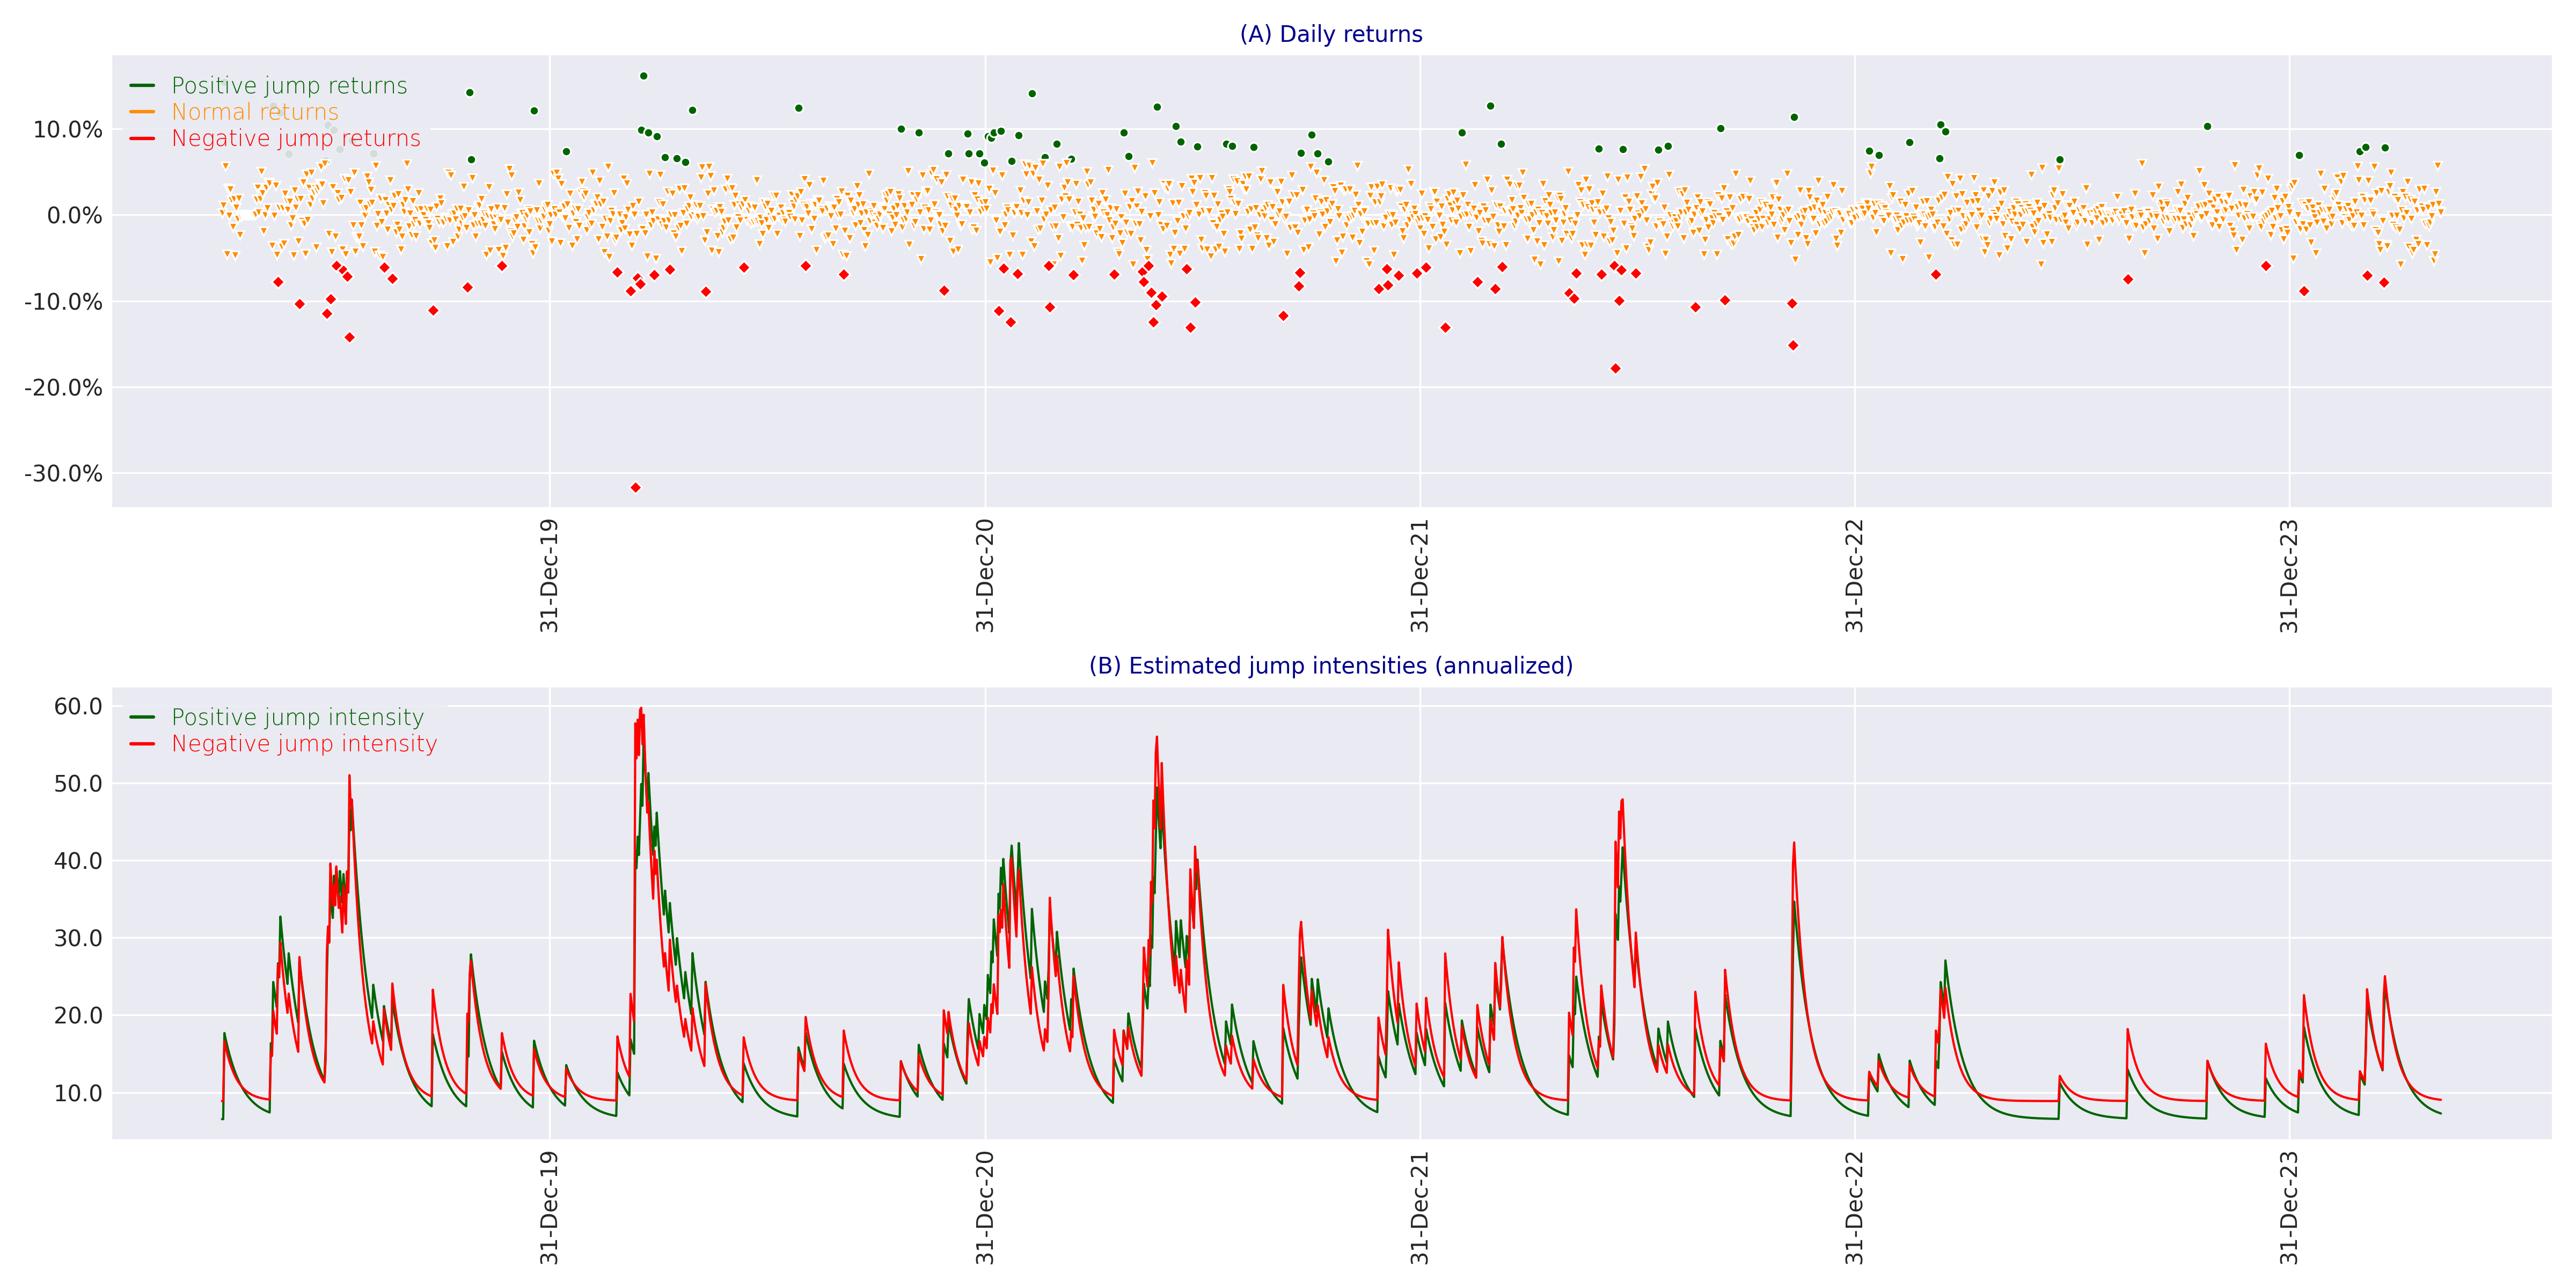
\includegraphics[width=1\linewidth]{figures/estimated_intensities.PNG}
    \label{fig:empirical?intensities}
\end{figure}

\begin{table}[t]
    \centering
\arraycolsep=1.4pt
$\begin{array}{lccrcccr}
      &   \multicolumn{7}{c}{\text{Parameter related to}}\\
    &\multicolumn{3}{c}{\lambda_t^+} &\phantom{\text{test}} & \multicolumn{3}{c}{\lambda_t^-} \\\hline
&\theta^+&=&5.7702 && \theta^-&=&8.5025\\
&\kappa^+&=&30.1413&& \kappa^-&=&18.3899\\
&\beta_{11}&=&174.3495 && \beta_{12}&=&-86.7846\\
&\beta_{21}&=&106.6187&& \beta_{22}&=&-87.9989\\
&\eta^+&=&0.0312&& \eta^-&=&0.0341\\
&\nu^+&=&0.0533&& \nu^-&=&-0.0462\\\hline
\text{Expected impact from}\\
\text{positive jump} &&& 14.7356 &&&& 9.0112\\
\text{negative jump} &&& 6.9655 &&&& 7.063\\
\end{array}
$
    \caption{Calibrated parameters of the jump intensities under $\mathbb P$.}
    \label{tab:calibrated}
\end{table}

The joint relevance of the cross-excitation parameters $\beta_{12}$ and $\beta_{21}$ is assessed by a likelihood ratio-test. The null hypothesis $H_0:\ \beta_{12}=\beta_{21}=0$ is rejected against the alternative $H_1:\ (\beta_{12},\beta_{21}) \neq (0,0)$ with a $p$-value of $4.1\cdot 10^{-8}$, where the likelihood-ratio test statistic is calculated from the full sample of BTC returns on the fully calibrated model and a reduced model with $\beta_{12}=\beta_{21}=0$.

\subsection{Calibration to market implied volatilities}\label{sec:second_stage}
For every day, given a set of European option prices and corresponding set of implied volatilities, we deduce volatility $\sigma$, and risk premia $\chi^+$ and $\chi^-$ by minimising the mean absolute percentage error (MAPE) as follows:
 \begin{align*}
  \left(\widehat \sigma,\ \widehat \chi^+,\ \widehat\chi^-\right) = \underset{\sigma,\chi^+,\chi^-} {\text{argmin}}
  \sum_{i=1}^I
  w_i \frac{\left|\text{IV}_{\text{market}}\left(\tau_i,\ K_i,\ O_i\right)-\text{IV}_\text{model}\left(\tau_i,\ K_i,\ O_i;\ \sigma,\ \chi^+,\ \chi^-\right)\right|}{\text{IV}_{\text{market}}\left(\tau_i,\ K_i,\ O_i\right)},
 \end{align*}
 where $I$ is the sample size, $w_i$ is the weight applied to the $i^\text{th}$ option,
 $\text{IV}_\text{market}\left(\tau_i,\ K_i,\ O_i\right)$ is the Black-Scholes (BS) implied volatility of the $i^\text{th}$ option with time-to-maturity $\tau_i$, strike $K_i$, and option type $O_i\in \left\{\text{Call},\ \text{Put}\right\}$. Here,
 $\text{IV}_\text{model}\left(\tau_i,\ K_i,\ O_i;\ \sigma,\ \chi^+,\ \chi^-\right)$ is the corresponding BS implied volatility produced by our model given $\sigma$, $\chi^+$, and $\chi^-$.
 We take the market BS vega of each option as weight $w$, thus assigning greater importance to options whose prices are more sensitive to mispricing of implied volatilities.

The computation of model implied volatilities given $\sigma$, $\chi^+$ and $\chi^-$ consists of the following steps.

\begin{enumerate}
    \item Compute $\lambda^{\pm,\mathbb{Q}}_t$, $\kappa^{\pm, \mathbb{Q}}$, $\theta^{\pm, \mathbb{Q}}$, $\beta_{ij}^\mathbb{Q}$ for $i,j\in [1,2]$, and $\eta^{\pm, \mathbb{Q}}$ using transformation in Equation~\eqref{eq:mgf_q1}.

    \item Apply the MGF under $\mathbb{Q}$ in Equation~\eqref{eq:mgf_q} along with risk-neutral drift $r$ and volatility $\sigma$ to value call and put options using Equation~\eqref{eq:opt1}.
    \item Infer model implied volatilities by inverting the Black-Scholes formula.
\end{enumerate}
We use a numerical optimiser to estimate $\widehat \sigma,\ \widehat \chi^+,\ \widehat\chi^-$ that minimise the MAPE.

Throughout, the estimated parameters satisfy condition (C1), so this constraint is non-binding.

\subsection{Calibration procedure's capability in fitting BTC IV smiles}
\begin{figure}[!t]
    \centering
    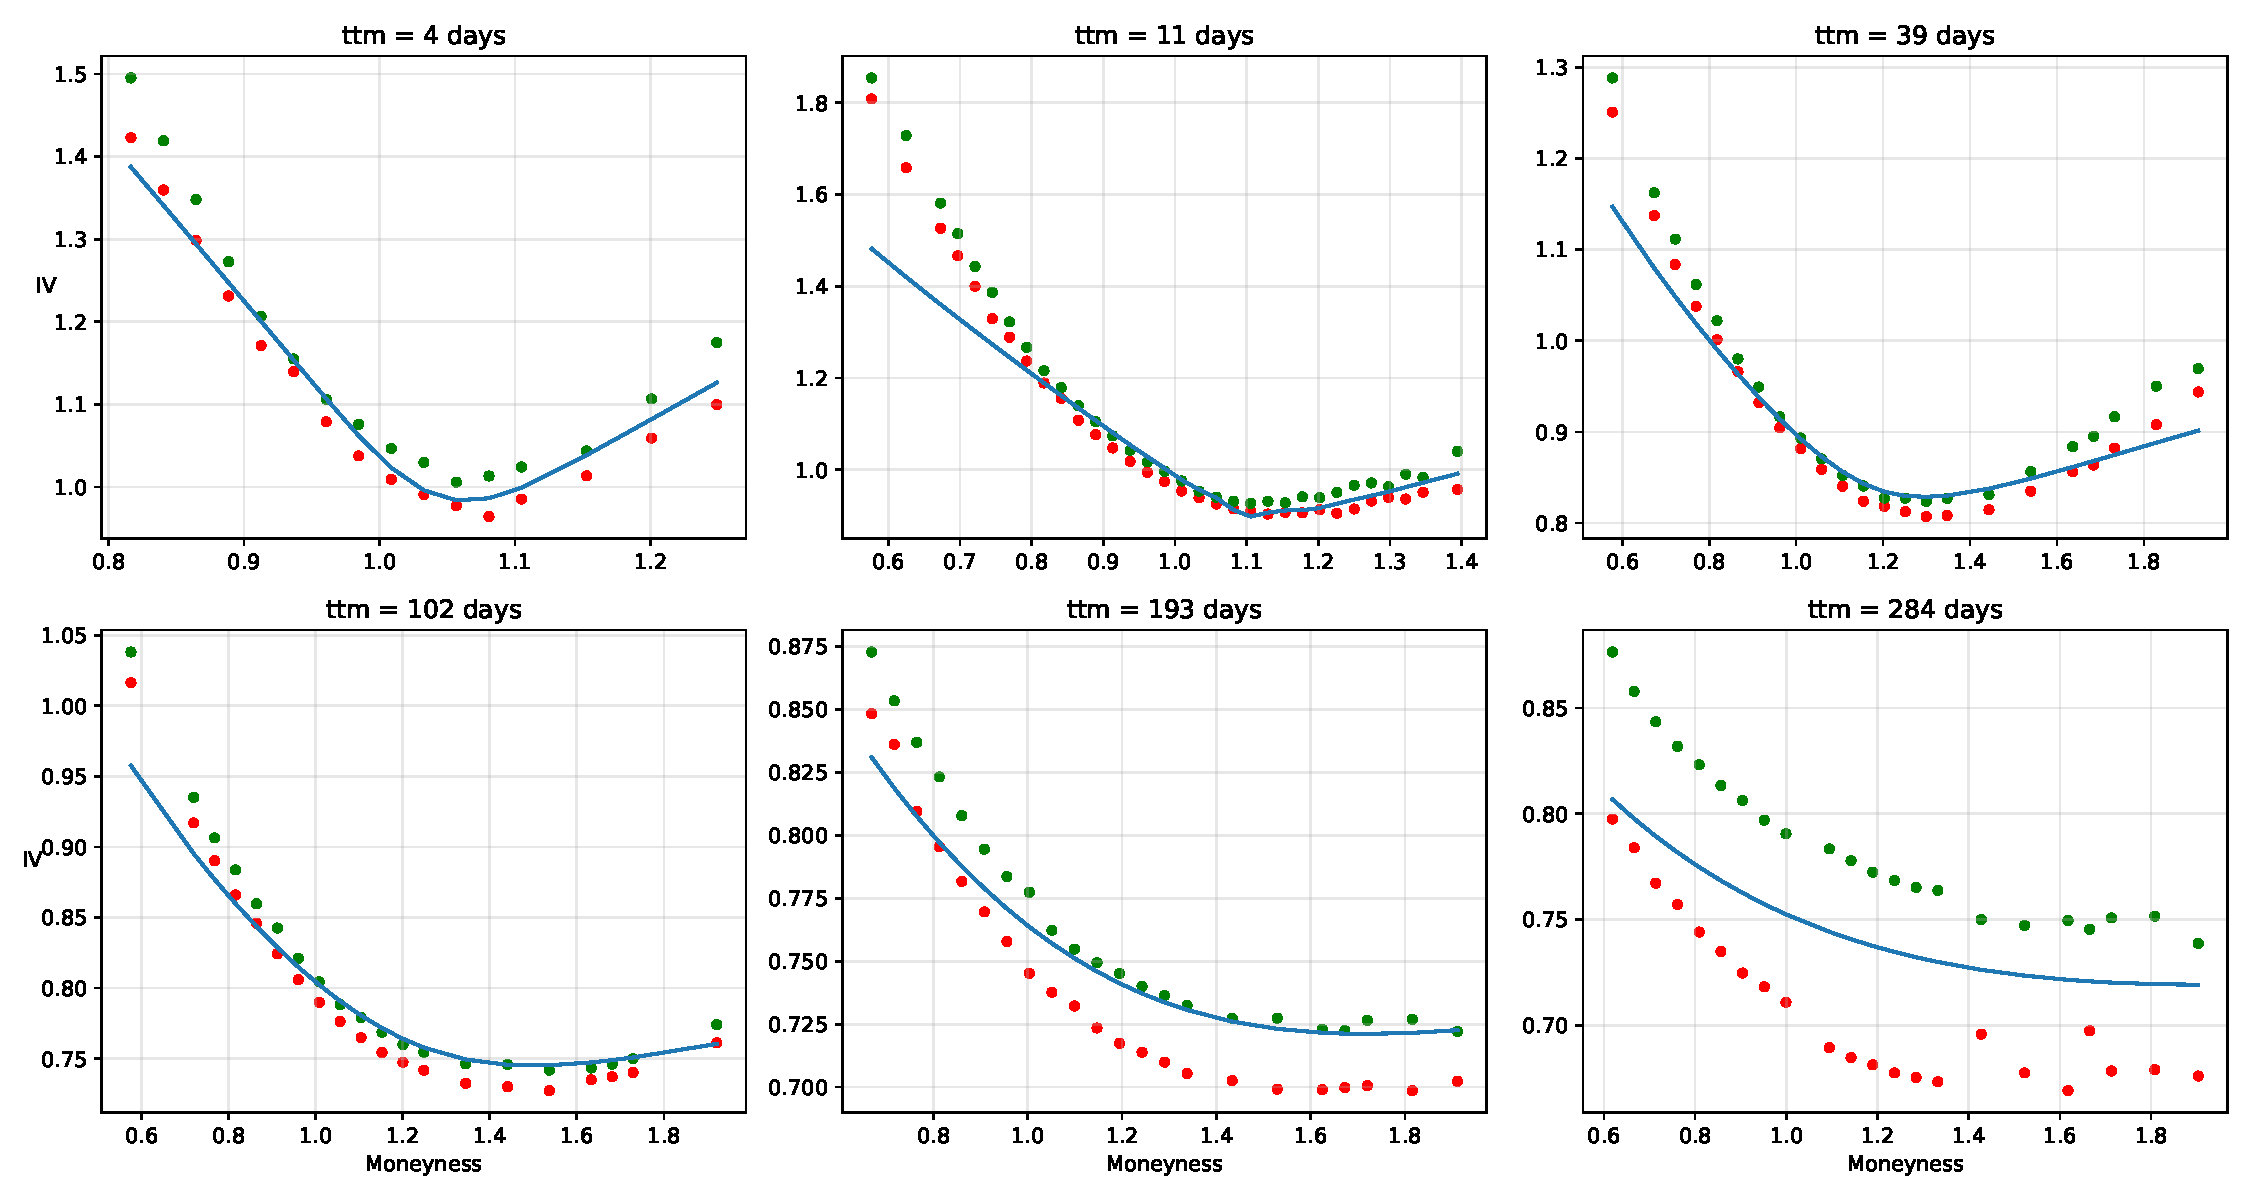
\includegraphics[width=\linewidth]{figures/2022-06-20_IV_calibration_results.pdf}
    \caption{Implied-volatility calibration on 2022-06-20 across six maturities. Bid and ask IVs are in green and red, respectively. The model IV is illustrated as the blue curve. The model matches the central region of the smile reasonably well, but deviations remain in the wings, especially for longer maturities.}
    \label{fig:iv_calibration_2022_06_20}
\end{figure}

\begin{table}[!t]
\centering
\caption{Calibration results for the BTC option smiles on 2022-06-20.}\label{tab:calibration_params_2022_06_20}
\begin{tabular}{rrrrrrr}
\toprule
ttm days & $\hat{\sigma}$ & $\hat{\chi}^+$ & $\hat{\chi}^-$ & $\hat{\gamma}^+$ & $\hat{\gamma}^-$ & MAPE \% \\
\midrule
4   & 0.4392 &  1.7411 & -7.0268 &  0.4406 & -3.3922 & 1.2432 \\
11  & 0.0500 &  0.7494 & -6.9411 &  0.1788 & -3.3273 & 3.1133 \\
39  & 0.0909 & -0.9643 & -5.0388 & -0.2088 & -2.0791 & 3.6799 \\
102 & 0.0300 & -1.8230 & -3.8149 & -0.3766 & -1.4383 & 3.0606 \\
193 & 0.0276 & -1.4132 & -3.1155 & -0.2985 & -1.1178 & 2.4691 \\
284 & 0.0279 & -0.9988 & -2.7709 & -0.2158 & -0.9706 & 1.9351 \\
\bottomrule
\end{tabular}
\end{table}

\begin{figure}[!t]
    \centering
    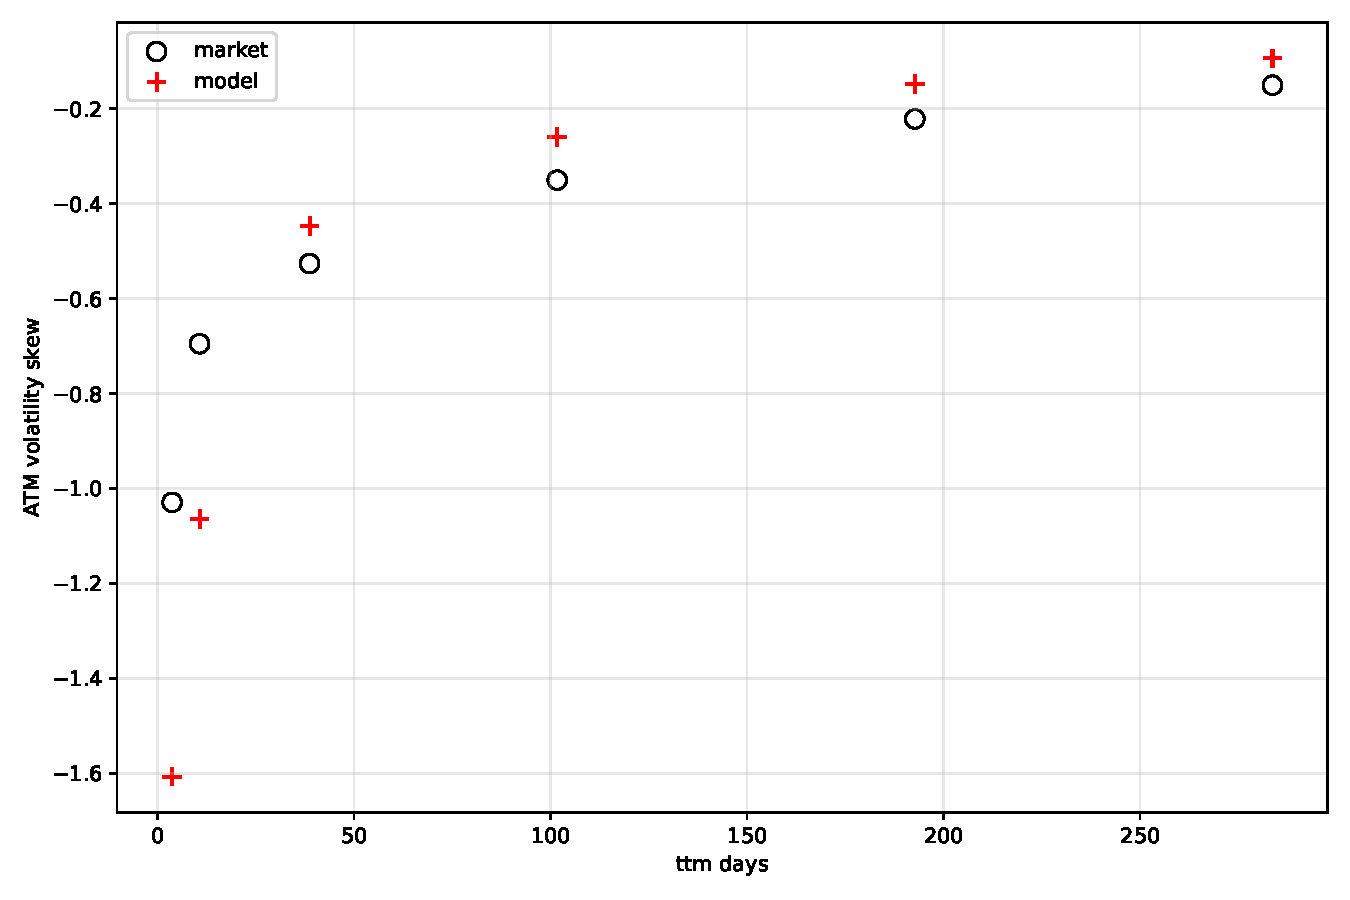
\includegraphics[width=.65\linewidth]{figures/2022-06-20_skewness.pdf}
    \caption{ATM volatility skews on 2022-06-20 across six maturities. }
    \label{fig:vol_skew_calibration_2022_06_20}
\end{figure}
Figures~\ref{fig:iv_calibration_2022_06_20} and \ref{fig:vol_skew_calibration_2022_06_20} show the model fit on 2022-06-20 across six maturities ranging from 4 to 284 days.
This date marks a period of particularly pronounced negative implied skewness in the sample.
The physical measure $\mathbb{P}$ is first estimated from daily BTC log returns over the period 2019-05-30 to 2022-06-20. Conditional on the $\mathbb{P}$-parameters, the risk-neutral parameters $\hat{\sigma}$, $\hat{\chi}^+$, and $\hat{\chi}^-$ are then calibrated to the BTC IV snapshot observed on 2022-06-20 at 9am UTC. Each smile, that is, each maturity slice, is calibrated separately.

The calibration performs reasonably well in the central region of the smile. In Figure~\ref{fig:iv_calibration_2022_06_20}, the model captures the level, curvature, and overall skewness in the near-at-the-money region for all maturities. The short term, in particular the 4-day and 11-day maturities, exhibits a pronounced smile, which is reproduced fairly well near the minimum. The fit remains acceptable at intermediate maturities such as 39 and 102 days.
The model tends to miss the slope of the smile away from the centre, with the right wing already slightly underestimated at 11 and 39 days. This becomes more visible for the 193- and 284-day maturities, where the model captures the overall level of the smile but not the full steepness of the wings.

Table~\ref{tab:calibration_params_2022_06_20} supports this assessment. The MAPE ranges from $1.24\%$ for the 4-day maturity option to $3.68\%$ for the 39-day maturity options, while the remaining maturities lie mostly between $2\%$ and $3\%$. This is consistent with a calibration that captures the dominant cross-sectional shape of the smile, but does not deliver a uniformly tight fit across the surface. Moreover, the estimated values of $\hat{\chi}^+$, $\hat{\chi}^-$, $\hat{\gamma}^+$, and $\hat{\gamma}^-$ do not display a clear monotone trend or an obvious term-structure pattern across maturities. The parameter estimates vary from one expiry to another, suggesting that the maturity dimension is not governed by a simple, stable structure in this calibration.

Figure \ref{fig:vol_skew_calibration_2022_06_20} reports the ATM volatility skew as defined e.g.\ Section 5 of \cite{dupret2023impact}. The model captures the ATM skews satisfactorily beyond the very short end, but it overstates the skew magnitude for the smallest maturities. For intermediate and longer maturities, the fit becomes materially better and follows the market term structure much more closely. The associated residuals are clearly structured rather than random, with a sign flip across maturity: they are negative at the shortest maturities and positive thereafter. This indicates that the model reproduces the global decay of the ATM skew, but does not fully capture the ultra-short-maturity behaviour. Such a pattern is not unexpected here, since the calibration was performed on implied-volatility smiles with shortest maturity close to one month, so that the short-end skew is not directly pinned down by the calibration data. This is also consistent with the evidence reported in \cite{dupret2023impact}, where the short-maturity ATM skew is shown to be particularly difficult to match with stochastic-volatility models, whereas the fit improves at longer maturities.

\section{Positive and negative jump risk premia}\label{sec:jumps_premia}

Following the literature on variance risk premia \citep[e.g.][]{Carr2009,bollerslev2009expected,almeida2024risk}, we define jump risk premia as the difference between expected jump sizes under the statistical measure and expected jump sizes under the risk-neutral measure.

\begin{corollary}[Using Proposition \ref{prop:risk-neutralisation}]
The positive jump risk premium denoted by $\gamma^+_t$ and negative jump risk premium denoted $\gamma^-_t$ are specified by:
\begin{align}
    \gamma^+_t & = \lambda^{+, \mathbb{Q}}_t \E^\mathbb{Q}\big(e^{J^{+,\q}}-1\big) -  \lambda^{+}_t \E\big(e^{J^+}-1\big),\label{eq:gamma_p}\\
    \gamma^-_t &= \lambda^{-, \mathbb{Q}}_t \E^\mathbb{Q}\big(e^{J^{-,\q}}-1\big) -  \lambda^{-}_t \E\big(e^{J^-}-1\big)\label{eq:gamma_m}.
\end{align}
\end{corollary}

According to the model specification for the price process in Equation~\eqref{eq:dS},
the terms $\lambda_t^+\E(e^{J^+}-1)$ and $\lambda_t^-\E(e^{J^-}-1)$ are the compensators for positive and negative jumps under statistical measure $\p$, respectively. By Proposition \ref{prop:HawkesUnderQ}, the parameters $\chi^+$ and $\chi^-$ in Equation~\eqref{eq:chi} specify compensators $\lambda^{+, \mathbb{Q}}_t \E^\mathbb{Q}\big(e^{J^{+,\q}}-1\big)$ and $\lambda^{-, \mathbb{Q}}_t \E^\mathbb{Q}\big(e^{J^{-,\q}}-1\big)$ under the risk-neutral measure $\q$. Hereby, the parameters $\chi^+$ and $\chi^-$ are inferred from options data.

In this construction, the jump risk premia reflect the difference in forward-looking risk preferences inferred from option prices compared to risk preferences inferred from historical price dynamics. Positive $\gamma_t^+$ and negative $\gamma_t^-$ indicate that the market expects higher future jump risk than was observed in the past, and vice versa for negative $\gamma_t^+$ and positive $\gamma_t^-$.
The jump risk premia are expressed in the same units as the drift rate $\mu$, i.e., as an annualised yield rate.

The separate treatment of positive and negative jumps is motivated by the fact that the market reacts differently to up and down moves in the price process. In particular, the left tail of the risk-neutral distribution is known to be more vulnerable to market downturns than the right tail to market upswings.  This is also seen in the impulse response functions in Section \ref{sec:jumps_premia_evolution} below, where the responses of positive and negative jump risk premia differ in magnitude and speed of decay in impact.

Figure \ref{fig:IV_smiles_varying_gammas} depicts the impact of jump risk premia on the implied volatility profiles of model-generated options with one month to maturity.
Generally, the magnitude of the jump risk premia is directly correlated with the overall level of model implied volatilities.
A higher positive jump risk premium and a lower negative jump risk premium contribute to a higher level of model implied volatilities.
However, as the panel on the top left reveals, the influence of
$\gamma^+$ is more pronounced on options with a moneyness greater than
1, predominantly in-the-money (ITM) call options.
The panel on the right shows the effect of the negative jump risk premium, where one has to bear in mind that a negative $\gamma^-$ indicates that more negative jump activity is expected under $\q$ than under $\p$. In turn, the more negative the $\gamma^-$ is, the higher the level of the model implied volatilities.
Similarly, this change in $\gamma^-$ shows a stronger impact on options with a moneyness less than 1, typically where the ITM put options are concentrated.

Figure \ref{fig:RND_variation_under_diff_jump_premia} illustrates the impact of $\gamma^{+}$ and $\gamma^{-}$ on the risk-neutral probability density of one-month log returns. The figure reveals that $\gamma^{+}$ and $\gamma^{-}$ jointly govern the asymmetry and tail thickness of the risk-neutral density, encapsulating the market’s pricing of upward and downward jump risks.

\begin{figure}[!t]
    \caption{
        The panels show model implied volatilities of one-month-maturity options under different positive and negative jump risk premium levels while keeping the opposite jump risk premium zero.
        The levels of positive jump risk premium are indicated to the right of the corresponding model implied volatilities. The model implied volatilities in red are under zero positive and negative jump risk premia. \href{https://github.com/QuantLet/HJP/tree/main/codes/jupyterNotebooks/IV_smiles_under_diff_risk_premia_level}{
\includegraphics[height=\baselineskip]{figures/qletlogo_tr.png}IV\_smiles\_under\_diff\_risk\_premia\_level}
    }
    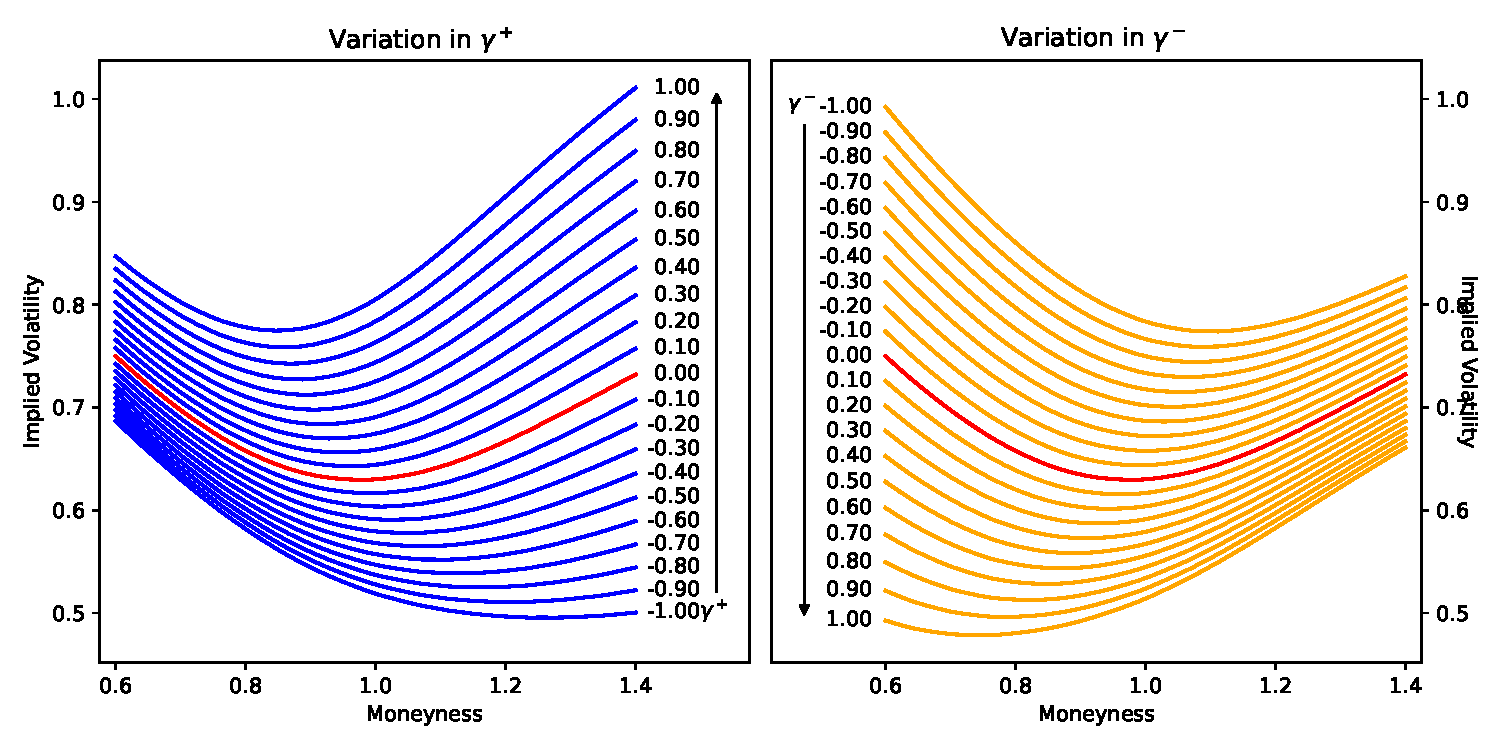
\includegraphics[width=\textwidth]{figures/IV_smiles_varying_gammas.pdf}
    \label{fig:IV_smiles_varying_gammas}
\end{figure}

\begin{figure}[!t]
    \caption{
        The panels display the risk-neutral probability densities of one-month log return under varying levels of the positive and negative jump risk premia, $\gamma^{+}$ and $\gamma^{-}$. The left panel illustrates the effect of changes in risk premia for calls $\gamma^{+}$ while holding $\gamma^{-}=0$, and the right panel shows the effect of changes in risk premia for puts $\gamma^{-}$ while holding $\gamma^{+}=0$. Increasing $\gamma^{+}$ fattens the right tail of the distribution, leading to greater right-skewness in the distribution. In contrast, variation in $\gamma^{-}$ produces the opposite pattern: a fatter or thinner left tail depending on the sign of the premium. Together, $\gamma^{+}$ and $\gamma^{-}$ govern the asymmetry and tail behavior of the risk-neutral density, reflecting how markets price the risk of upward and downward jumps.
    }
    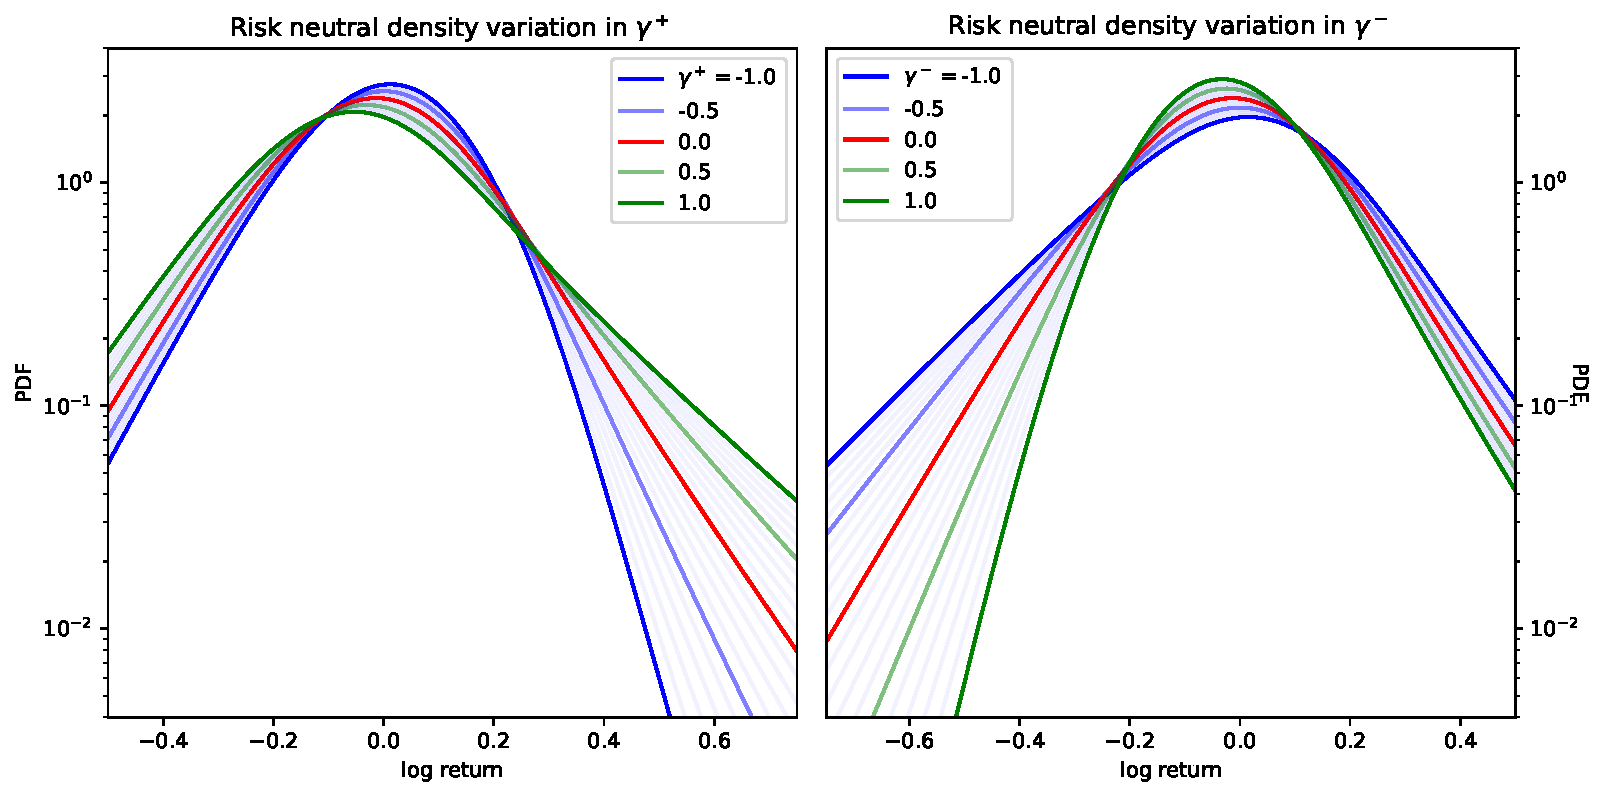
\includegraphics[width=\textwidth]{figures/narrower_x_RND_variation_under_diff_jump_premia.pdf}
    \label{fig:RND_variation_under_diff_jump_premia}
\end{figure}

\section{Empirical Results}\label{sec:results}
\subsection{Data and empirical study design}
We study the options market for cryptocurrencies, with its dynamics heavily influenced by sentiment-driven jumps and severe price adjustments. In particular, we consider options on Bitcoin (BTC) which are the most liquid in cryptocurrency derivatives. We gather data on both BTC price and BTC options from Deribit, a crypto derivatives exchange established in June 2016. The exchange offers options and futures trading for both BTC and ETH and provides extensive data on BTC prices and option prices through its API. Deribit's comparatively low fees for market makers contribute to the open interest and transaction volume for options traded on the platform.

Our sampled BTC price data spans from 2015-12-31 to 2023-10-04 with the sample of BTC opening prices at 9 am UTC. As for the BTC options data, our collection starts from 2019-05-30 to 2023-10-04. The options data consists of 9 am UTC snapshots of the bid and ask IVs of call and put options. We chose to capture these snapshots at 9 am UTC to minimise the impact of market fluctuations that often occur due to the introduction of new options and futures listings at 8 am UTC.

We split the data into two datasets based on the availability of one-month option data. The first dataset is data observed from 2015-12-31 to 2019-05-29, where 2019-05-30 is the earliest date when 1-month options became available on Deribit. The second dataset is data observed from 2019-05-30 onward.

We design the empirical study as follows.
Initially, we use BTC price data from the first dataset for the estimation of model parameters that are associated with jumps, as described in Section \ref{sec:two_stage}.
In this stage, we apply POT estimation to filter out arrival times and magnitudes of positive and negative jumps in the BTC price in the testing data.
 In this empirical study, the training data are the daily BTC price observed from 2015-12-31 to 2019-05-29.
From the time series of BTC price, we compute the jump intensities for the training data, and then generalise the computation of intensities to the testing data based on the estimated model parameters.
The model parameters are held fixed to infer jump intensities to enforce no look-ahead bias in our empirical results.

Once a set of model parameters is estimated and the time series of jump intensity rates are inferred, we calibrate model volatility $\sigma$, and risk premium parameters $\chi^+$ and $\chi^-$ using options data in the second dataset.
Options data include mid quotes of implied volatilities of call and put options, specifically options with maturities that are closest to, but less than one month, and have a moneyness range between 0.8 and 1.2. These options are characterised by high open interest and high transaction volume.

The final step involves the analysis of the jump risk premia computed using Equations~\eqref{eq:gamma_p} and \eqref{eq:gamma_m}. Section \ref{sec:jumps_premia_evolution} presents the evolution of jump risk premia together with the main events in the BTC market. Section \ref{sec:cost_of_carry} reports the relationship between the jump risk premia and the cost-of-carry of BTC futures. Section \ref{sec:PnL_realisation} shows application of the jump risk premia to profit and loss of delta-hedged option strategies.

\subsection{Goodness-of-fit}\label{sec:gof}
We visually assess the goodness of fit of our model to the BTC price dynamics through Q-Q plots of the inter-arrival times of unit rate Poisson processes versus the transformed inter-arrival times of observed BTC price jumps,
 $\int_{T^+_{[k-1]}}^{T^+_{[k]}}\lambda^+_s \text{d}s$ for $k = 1,2,...,N^{(1)}$ and $\int_{T^-_{[k-1]}}^{T^-_{[k]}}\lambda^-_s \text{d}s$ for $k = 1,2,..., N^{(2)}$, where $N^{(1)}$ and $N^{(2)}$ are the numbers of positive and negative jumps observed until time $T$.
Appendix \ref{sec:QQplot} provides further details of this approach.

Figure \ref{fig:QQPlot_lambdas} presents the Q-Q plot of the model estimates. Model parameters are estimated from 2015-12-31 to 2019-05-29, as mentioned above. These estimates are applied to transform the jumps arrival times of the whole dataset from 2015-12-31 to 2023-10-04. In the Q-Q plots, data points from the first dataset are marked by circles, data points from the testing data are marked by crosses. The model estimates fit reasonably well for most of the negative jumps inter-arrival times.
While the model also fits most positive-jump inter-arrival times reasonably well, the Q-Q plot reveals a noticeable upper-tail deviation, with overestimation for theoretical quantiles above approximately 3. Many of these deviations arise in the out-of-sample period after 2019-05-30. One possible explanation is that upward BTC jumps are harder to predict than downward jumps. \citet{Zhang2023} show that self-excitation in Bitcoin returns is stronger for bad (negative) jumps than for good (positive) jumps, while \citet{SaefEtAl2024} documents that negative jumps are more prevalent and exhibit stronger temporal clustering in cryptocurrency markets, especially for Bitcoin. This suggests that negative jumps are easier to capture with parameters estimated from a historical training sample, whereas positive jumps may be more sensitive to the choice of estimation window and jump-identification procedure. To improve the calibration quality, a natural improvement is to calibrate the model more frequently. Relatedly, the positive-jump component can be re-estimated using rolling or expanding windows, and greater weight could be assigned to recent observations when inferring positive-jump intensities.

\begin{figure}
    \caption{
        The left panel shows the Q–Q plot of compensator-transformed interarrival times for positive jumps; the right panel shows the same for negative jumps. Circles and crosses  represent jumps occurring before (in-sample) and after (out-of-sample) 2019-05-30, respectively. Under the model, the transformed interarrival times should follow a standard exponential distribution. The model is calibrated on data before 2019-05-30, and the estimated parameters are used to infer intensities for periods after 2019-05-30. The close agreement between theoretical and empirical quantiles indicates strong in- and out-of-sample performance.
\href{https://github.com/QuantLet/HJP/tree/main/codes/jupyterNotebooks/goodness_of_fit_P}{
\includegraphics[height=\baselineskip]{figures/qletlogo_tr.png}goodness\_of\_fit\_P}
    }
    \label{fig:QQPlot_lambdas}
    \begin{center}
    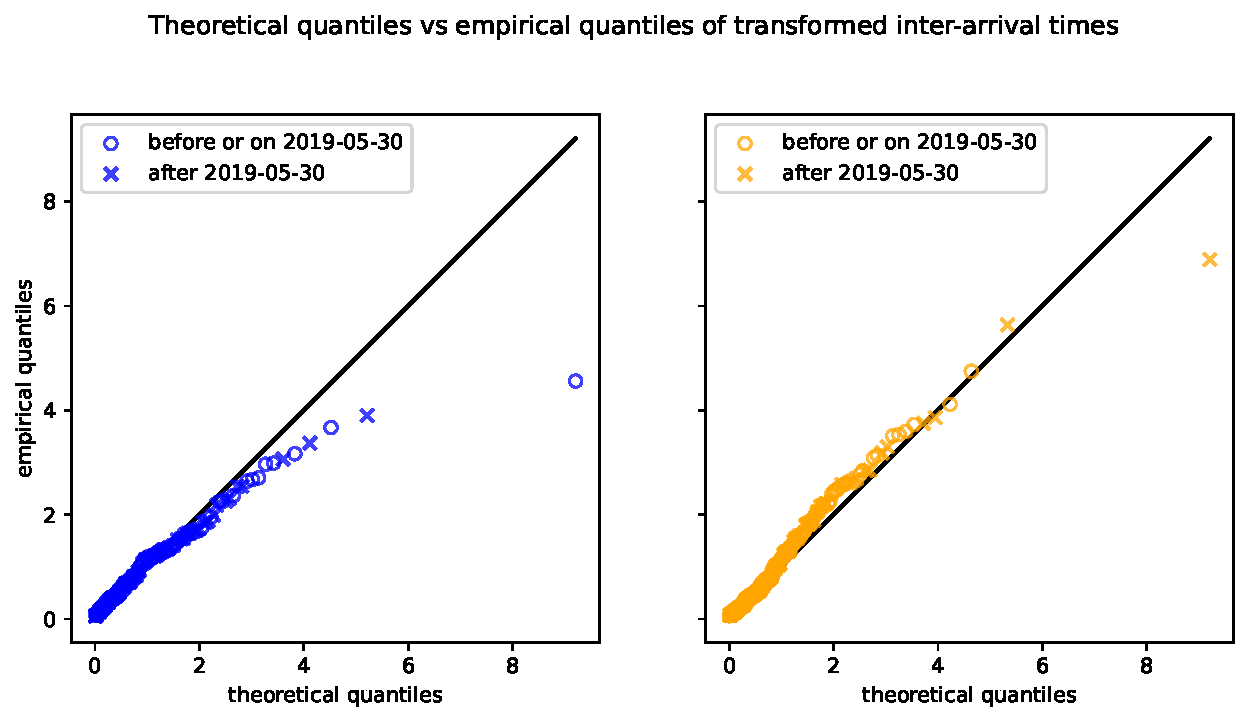
\includegraphics[width=\textwidth]{figures/QQ_plots.pdf}
    \end{center}
  \end{figure}

  {
\subsection{Verification of conditions (C1)--(C3) on the calibration sample}
\label{sec:verif}

Conditions (C1) and (C2) depend on the calibrated risk-premium pair
$(\chi^{+}_{t_k},\chi^{-}_{t_k})$ and are verified on each of the $K=1588$ calibration dates in the
sample (2019-05-30 to 2023-10-04); the calibrated premia span $\chi^{+}\in[-32.1,8.7]$ and
$\chi^{-}\in[-11.3,29.4]$ (medians $-1.2$ and $-1.3$).

\emph{(C1) admissibility.} The margins $m^{+}_{t_k}:=1-\eta^{+}\chi^{+}_{t_k}$ and
$m^{-}_{t_k}:=1+\eta^{-}\chi^{-}_{t_k}$ are strictly positive on \emph{every} date, with smallest
values $\min_k m^{+}_{t_k}=0.73$ and $\min_k m^{-}_{t_k}=0.62$. By
Proposition~\ref{prop:true_mg} and Remark~\ref{remark:6.3} this alone secures the true-martingale property of
$M$ --- and hence the validity of the measure change and of the option-pricing formula --- on the
entire sample.
Condition (C3) therefore needs no separate diagnostic: it follows from (C1)
(Remark~\ref{remark:6.3}), and is corroborated by the integration of the $R^{*}$-system~\eqref{eq:Rstar} without
explosion at every date during pricing.

\emph{(C2) $\q$-stationarity.} We compute the spectral abscissa $s(\Phi^{\q}_{t_k})$ of the risk-neutral first-moment matrix in condition (C2), evaluated at the date-$t_k$ calibrated parameters. The
condition $s(\Phi^{\q}_{t_k})<0$ holds on $1459$ of the $1588$ dates ($91.9\%$). The $129$
exceedances are concentrated in the elevated-sentiment regime of 2021 ($21.9\%$ of that year) and
arise when the calibrated premia are large enough that the risk-neutral self-excitation of one jump
type exceeds its mean-reversion rate, rendering the $\q$-intensities locally non-stationary. As
emphasised in Remark~\ref{remark:6.2}, (C2) governs first-order stationarity of the intensities under $\q$ ---
relevant for unconditional and long-horizon $\q$-moments --- and is \emph{not} required for the
martingale property: on these dates the measure change is still admissible by (C1) and $M$ is still a
true martingale by (C3). Table~\ref{tab:verification} reports the minimum, median and maximum of the three
diagnostics across all dates.

\begin{table}[h!]
\centering\small
\begin{tabular}{lllcccc}
\toprule
Condition & Diagnostic & Req. & Min & Median & Max & Holds\\
\midrule
(C1) & $m^{+}=1-\eta^{+}\chi^{+}$ & $>0$ & $0.73$ & $1.04$ & $2.00$ & $1588/1588$\\
(C1) & $m^{-}=1+\eta^{-}\chi^{-}$ & $>0$ & $0.62$ & $0.96$ & $2.00$ & $1588/1588$\\
(C2) & $s(\Phi^{\q})$ (spectral abscissa) & $<0$ & $-17.04$ & $-4.38$ & $+11.34$ & $1459/1588$\\
\bottomrule
\end{tabular}
\caption{Verification of (C1)--(C2) across all $1588$ calibration dates (2019-05-30 to 2023-10-04).
(C1) holds throughout, which with (C3) (Remark~\ref{remark:6.3}) secures the true-martingale property on every
date. (C2) holds on $91.9\%$ of dates; the exceedances are high-sentiment 2021 regimes and, by
Remark~\ref{remark:6.2}, do not affect the martingale property.
\href{https://github.com/QuantLet/HJP/tree/main/codes/calibration_diagnostic}{
\includegraphics[height=\baselineskip]{figures/qletlogo_tr.png}calibration\_diagnostic}}
\label{tab:verification}
\end{table}
}

\subsection{Evolution of jump risk  premia} \label{sec:jumps_premia_evolution}

The dynamics of jump risk premia, computed using Equations~\eqref{eq:gamma_p} and \eqref{eq:gamma_m}, from 2019-05-30 to 2023-10-04 are illustrated in Figure \ref{fig:jps}.
Overall, the jump risk premia vary strongly over time, while showing a tendency to mean-revert to a mean close to zero. In addition,
the negative jump risk premium fluctuates in the same direction as the positive jump risk premium, but with a stronger magnitude. This co-movement suggests the time-varying skewness observed in option prices. When jump risk premia are negative and put options have a higher demand than call options, the implied volatility skew becomes left-skewed compared to the skew inferred by the statistical measure, and vice versa.

Although \cite{Bollerslev2011}'s data and methodology differ significantly from ours, their findings are in line with our results. Using high-frequency data and a model-free approach to decompose volatility into continuous and jump components, they found that investors demand a significantly higher premium for downside jump risk than for upside jump risk. This asymmetry supports our observation that negative jump risk premia tend to have a greater magnitude than positive premia. When pricing longer-dated options, the extremely high jump risk premia are not expected to last very long due to the mean reversion of jump intensities.

A significant peak in premia was observed on 2021-01-16, building on the increase that started in early October 2020, a period marked by heightened institutional activity and a series of all-time high break-outs for BTC price.
The troughs and the market situations during the time include the following (i) 2020-03-22: COVID-19 outbreak starting in March 2020; (ii) 2021-05-27: environmental concerns over Bitcoin mining; (iii) 2022-06-20: $40\%$ decline in BTC caused by hawkish interest rate policy of the U.S. Federal Reserve amid high inflation rates; (iv) 2022-11-15: the FTX crisis and subsequent crash of cryptocurrencies.

\begin{figure}
    \caption{
        The time series plots illustrate the positive and negative jump risk premia, depicted by light blue and light orange lines, respectively.
        The darker lines in the plots represent the seven-day moving averages of the corresponding jump risk premia.
        These moving averages reveal a more distinct pattern in the evolution of the jump risk premia.
        The jump risk premia are estimated from 2019-05-30 to 2023-10-04.
        \href{https://github.com/QuantLet/HJP/tree/main/codes/jupyterNotebooks/jumps_premia_evolution}{
\includegraphics[height=\baselineskip]{figures/qletlogo_tr.png}jumps\_premia\_evolution}
    }
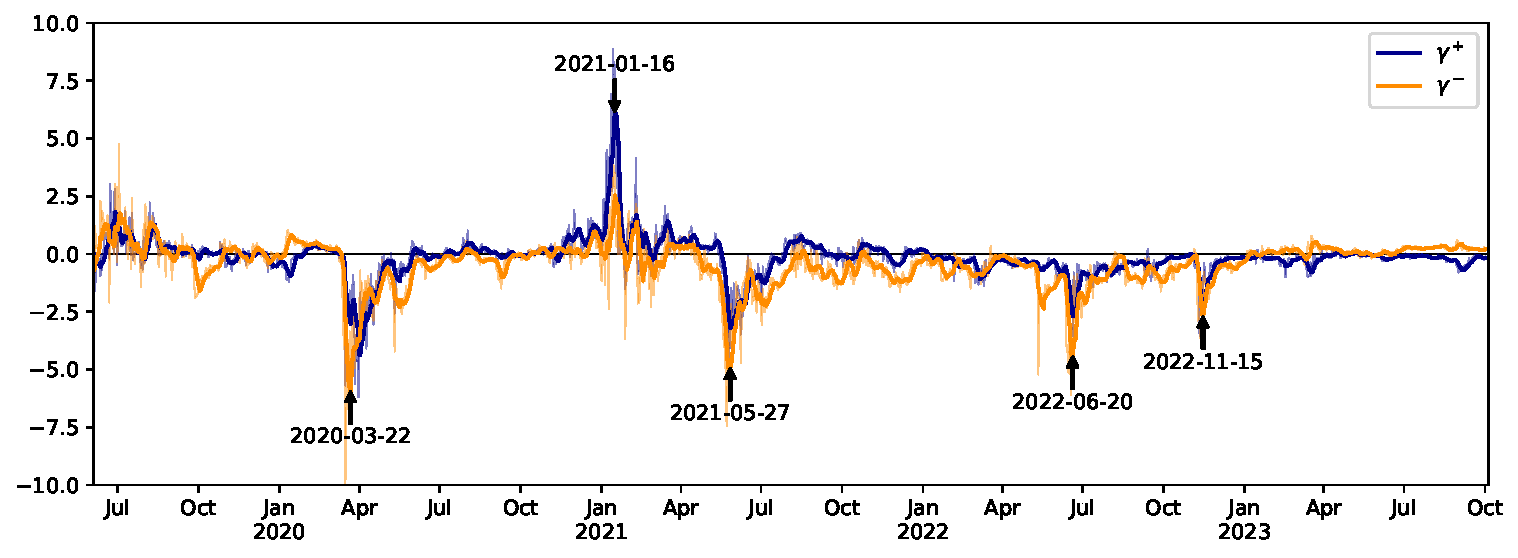
\includegraphics[width=\textwidth]{figures/jumps_premia.pdf}
\label{fig:jps}
\end{figure}

\subsection{Jump risk premia as factors in explaining BTC futures cost-of-carry}
\label{sec:cost_of_carry}

BTC futures are a popular choice for investors seeking leveraged exposures to BTC dynamics. Here, we investigate whether jump risk premia can serve as explanatory factors for BTC futures pricing, specifically through their relationship with the cost-of-carry.
The variable of interest is the BTC basis or cost-of-carry specified as follows:
\begin{align}
    c_t = \ln\big(F_t(\tau)/S_t\big)/\tau,
\end{align}
where $F_t(\tau)$ is the price at time $t$ of a futures contract with
time-to-maturity $\tau$, and $S_t$ is the spot price of BTC.
Figure \ref{fig:BTCfutures} shows the basis $c_t$, computed using the prevailing futures contract with a time-to-maturity just below one month, based on data from Deribit.
The cost-of-carry is annualized and exhibits high volatility, ranging from $-20\%$ to $80\%$. High values of the cost-of-carry arise when investors seek leverage. A trader can monetise a high value of the cost-of-carry by selling short the futures and going long BTC through a spot market.

\begin{figure}[!t]
    \caption{
        The time series plot shows the BTC futures basis $c_t$ observed in the market.
        The data is calculated using the price of the future with maturity $\tau$ less than, but closest to one month.
        \href{https://github.com/QuantLet/HJP/tree/main/codes/jupyterNotebooks/cost_of_carry_factors}{
\includegraphics[height=\baselineskip]{figures/qletlogo_tr.png}cost\_of\_carry\_factors}
    }
    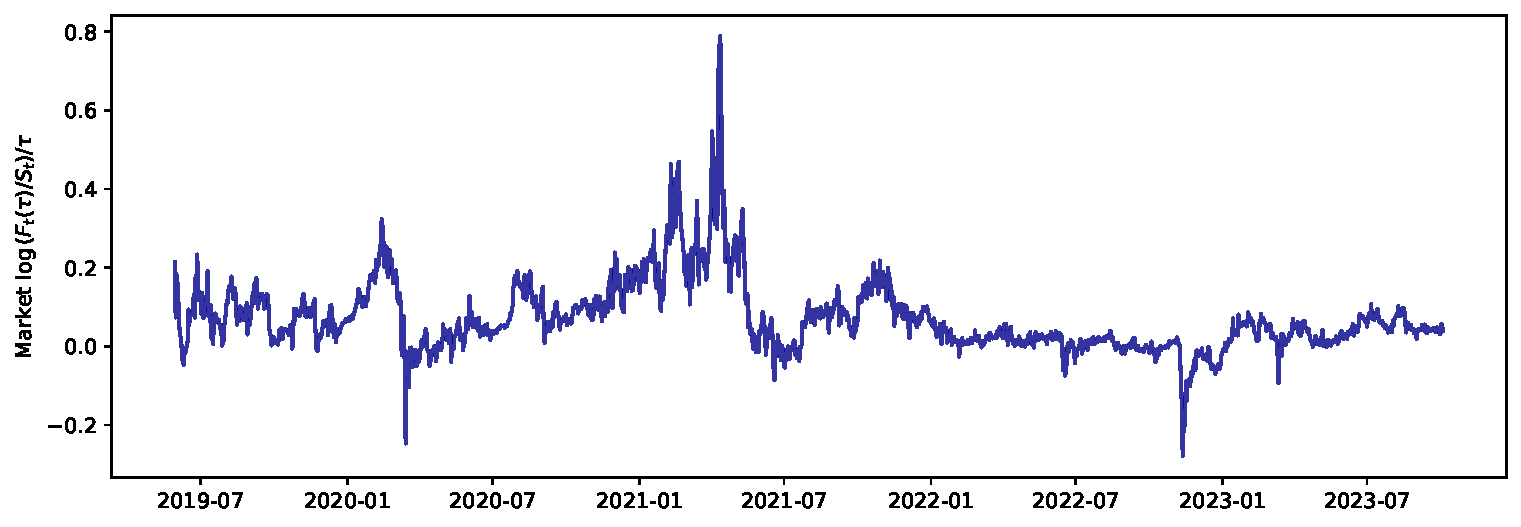
\includegraphics[width=\textwidth]{figures/futures_slope.pdf}
    \label{fig:BTCfutures}
\end{figure}

In addition to the jump risk premia, the number of positive and negative jumps in the previous week,
abbreviated respectively as $N^{(1)}_t - N^{(1)}_{t-7}$ and $N^{(2)}_t - N^{(2)}_{t-7}$, and the average funding rate of the week from Deribit BTC perpetual futures, abbreviated by $r^{\text{funding}}_{t, t-7}$, are included as independent variables in order to support the analysis.
The regression of interest is given by
\begin{align}
    \Delta c_t &=  \beta_1 \Delta \gamma^+_t + \beta_2 \Delta \gamma^-_t
    + \beta_3 \Delta \big(N^{(1)}_t - N^{(1)}_{t-7}\big)
    + \beta_4 \Delta \big(N^{(2)}_t - N^{(2)}_{t-7}\big)
    + \beta_5 \ \Delta r^{\text{funding}}_{t, t-7} + \Delta \varepsilon_t. \label{eq:regression_of_futures}
\end{align}

All variables are differenced to remove potential fixed effects and to mitigate the impact of any fixed effects.
To mitigate the noise arising from daily fluctuations and the introduction of new contracts, the data selected for the regression analysis consist of market snapshots captured every Friday at 9 am UTC.
This timing is chosen because traders typically adjust their positions on Fridays to manage risk for the upcoming weekend.
Additionally, newly issued options and futures contracts typically begin trading at 8 am, allowing the 9 am UTC snapshot to incorporate the initial market responses of these new instruments.
The variables are observed every Friday at 9 am UTC from 2019-06-14 to 2023-02-17.
Table \ref{tab:BTCfutures_regression} reports the estimated coefficients, Newey-West robustified $t$-statistics, and adjusted $R^2$ coefficients of regressions of $c_t$ on combinations of explanatory variables.

\begin{table}[!t]
    \caption{
        The table reports estimated coefficients, Newey-West robustified $t$-statistics,
        and adjusted $R^2$ coefficients of regressions of the futures basis $c_t=\ln(F_t(\tau)/S_t)/\tau$.
        The futures contract with time-to-maturity $\tau$ smaller than, but closest to one month is chosen for each observation time to represent the futures market.
        The regressors are defined as follows: $\gamma^+_t$ and $\gamma^-_t$ are the jump risk premium.
        $N^{(1)}_t - N^{(1)}_{t-7}$ and $N^{(2)}_t - N^{(2)}_{t-7}$ are number of positive and negative jumps in the week prior to $t$, respectively.
        $r^{\text{funding}}_{t, t-7}$ is the average funding rate of the week from Deribit BTC perpetual futures.
        The Deribit BTC funding rate is chosen to represent the convenience yield in the crypto market.
        All variables enter as first differences.
         $^{*}$, $^{**}$, and $^{***}$ indicate statistical significance at the 10\%, 5\%, and 1\% levels, respectively.
        The variables are observed every Friday at 9 am UTC from 2019-06-14 to 2023-02-17.
        \href{https://github.com/QuantLet/HJP/tree/main/codes/jupyterNotebooks/cost_of_carry_factors}{
\includegraphics[height=\baselineskip]{figures/qletlogo_tr.png}cost\_of\_carry\_factors}
    }
    \begin{center}
      \resizebox{\textwidth}{!}{
\begin{tabular}{rSSSSSS}
\toprule
{} &            I &            II &          III &           IV &            V &           VI \\
\midrule
$\gamma^+_t$         &  0.0157$***$ &               &              &  0.0160$***$ &       0.0071 &    0.0075$*$ \\
            &     (2.6139) &               &              &     (3.5339) &     (1.2400) &     (1.7027) \\
$\gamma^-_t$         &   0.0132$**$ &               &              &       0.0089 &   0.0131$**$ &    0.0097$*$ \\
            &     (2.2257) &               &              &     (1.4316) &     (2.5760) &     (1.7995) \\
$N^{(1)}_t - N^{(1)}_{t-7}$ &              &    0.0102$**$ &              &  0.0112$***$ &              &    0.0073$*$ \\
            &              &      (2.1840) &              &     (3.0709) &              &     (1.8356) \\
$N^{(2)}_t - N^{(2)}_{t-7}$ &              &  -0.0179$***$ &              &  -0.0126$**$ &              &  -0.0114$**$ \\
            &              &     (-2.8429) &              &    (-2.4792) &              &    (-2.2707) \\
$r^{\text{funding}}_{t,t-7}$          &              &               &  0.0024$***$ &              &  0.0020$***$ &  0.0018$***$ \\
            &              &               &     (4.6951) &              &     (3.8976) &     (3.7371) \\
\midrule
Adj. $R^2$ & 0.1467 & 0.0866 & 0.2231 & 0.1956 & 0.2794 & 0.3107\\\bottomrule
\end{tabular}
    }
    \end{center}
    \label{tab:BTCfutures_regression}
\end{table}

The results of the regression analysis reveal a significant explanatory power of jump risk premia in determining the volatile cost-of-carry for BTC futures.
In Regression I, the coefficients for jump risk premia are both positive and statistically significant.
This model yields an adjusted $R^2$ of 14.7\%, together with the significant coefficients, supporting the hypothesis that futures prices are directly proportional to the jump risk premia.

The jump risk premia explanatory power is robust against the presence of the number of jumps and the funding rate variables.
This conclusion is drawn by comparing the adjusted $R^2$ values and coefficients from Regression I with those from Regressions IV and V.
Combining the results of Regression I with that of Regression IV side by side, which includes the number of jumps from the previous week, the coefficient of the positive jump risk premium remains significant.
Inclusion of these variables improves the adjusted $R^2$ to 19.6\%.
However, the coefficient of the negative jump risk premium decreases in magnitude and becomes statistically insignificant in this context.
A similar pattern is noted in Regression V.
When the funding rate is included in the Regression V, the coefficient of negative jump risk premium slightly diminishes while remaining significant, but
the coefficient of positive jump risk premium halves and becomes statistically insignificant.
The inclusion of the average funding rate improves the adjusted $R^2$ to 28\%.
These improvements value of $R^2$ confirm that the number of jumps and the average funding rate provide additional information to explain the level of BTC futures cost-of-carry in addition to the jump risk premia.
However, the shrinkage of the magnitudes and loss in statistical significance observed from the coefficients are probably due to the correlation between the variables.
Empirically, the correlation between the positive jump risk premium and the funding rate is around $36.7\%$; the correlation between the negative jump risk premium and the number of negative jumps is around $-24\%$.

The interpretation of the correlations is as follows.
The positive correlation between the positive jump risk premium and the funding rate may be due to the increasing speculative demand for both call options and perpetual futures.
In contrast, the negative correlation between the negative jump risk premium and the number of negative jumps can result in higher put option prices during bearish periods with high volatility.
This interpretation is consistent with the findings of \cite{schmeling2023crypto}.
They attribute high cost-of-carry of BTC futures to the interaction between the trend-chasing behaviour of market traders and the scarcity of arbitrage capital that conducts cash-and-carry trade.

Regression VI offers a comprehensive overview of how jump risk premia affect BTC futures prices, taking into account all relevant variables.
This regression reaches an adjusted $R^2$ value of $31\%$, with each coefficient demonstrating statistical significance.
According to the regression result, a one-unit increase in the
positive jump risk premium is associated with a 0.75 basis point increase in the cost of carry of BTC futures $c_t$.
 Similarly, a one-unit increase in the negative jump risk premium corresponds to an increase of 0.97 basis points in $c_t$.
The positive signs of both the positive and negative jump risk premia coefficients in Regression VI indicate that a positive change corresponds to (forward-looking) option and futures market being more optimistic than the price history suggests.
The different sizes of the positive and negative jump risk premia coefficients can be attributed to risk aversion, as traders and investors are more sensitive to losses than to gains.

\subsection{Jump risk premia realisation}\label{sec:PnL_realisation}
In the spirit of \cite{carr1998towards} who quantify the return variance risk premium of an asset using the market prices of options, we answer the question of how the risk premia can be realised. To this end, we investigate whether the jump risk premia defined in Equations~\eqref{eq:gamma_p} and \eqref{eq:gamma_m} can explain the one-week-ahead returns of delta-hedged short-option strategies, following an empirical approach similar to \cite{bakshi2003delta}. The option strategies are constructed using the same data and approach as \cite{lucicsepp2024}, where short positions in calls, puts, straddles and strangles are delta-hedged using Black-Scholes (BS) deltas and rebalanced hourly until expiration.

All strategies are written on options expiring on the subsequent Friday at 8am UTC.
As both positive and negative jump risk premia are observed, we define simple trading signals as follows: A positive risk premium for positive jumps, which means that the market prices call options higher than implied by the historical measure, is considered an opportunity to sell call options and call spreads.
The trading decision is similar for put options and put spreads when observing a negative risk premium on negative jumps.
For portfolios involving straddle and strangles, which are combinations of call and put options, the trading strategy is to sell them if at least one of the risk premia is ``active'' in the sense described previously.
The trading signals for all strategies are determined on each Friday at 9am UTC, and if active, the position is created (and delta-hedged with hourly rebalancing) until expiry the following Friday. Long positions in calls and puts are not entered if the jump risk premia are ``reversed'' due to the loss in time value of the options (negative theta).

Using \cite{bakshi2003delta}'s empirical methodology, we investigate the relationship between jump risk premia as defined above and one-week-ahead returns of the option strategy portfolios.
This is achieved by conducting a regression of the one-week-ahead log returns $u_t= \ln(P_t/P_{t-1})$ of each strategy, with $P_t$ the option strategy value at time $t$, against the jump risk premia. Essentially, $u_t$ expresses the hedge error from hedging using a Black-Scholes delta from market-implied volatilities.
The regression of interest is
\begin{equation}
    u_{t+1} = \beta_0 + \beta_1 \gamma^+_t + \beta_2 \gamma^-_t %
     + \beta_3 \Delta \gamma^+_t + \beta_4 \Delta \gamma^-_t %
     + \beta_5 (N^{(1)}_t-N^{(1)}_{t-1})
    + \beta_6  (N^{(2)}_t-N^{(2)}_{t-1}),
    \label{regression_optionstrategies}
\end{equation}
where $u_{t+1}$ is the one-week-ahead options strategy return at time $t$ (expressed in basis points),
$\Delta$ is the first difference operator and
$(N^{(1)}_t-N^{(1)}_{t-1})$ and $(N^{(2)}_t-N^{(2)}_{t-1})$ count the number of jumps that occurred within the previous week.
The option strategies of interest are delta-hedged short-option strategies of different moneyness, as follows:
\begin{enumerate}[label=(\roman*)]
\item ATM: calls and puts with at-the-money strikes;
\item 10D: options with delta of +0.1 for calls and -0.1 for puts;
\item 25D: options with delta of +0.25 for calls and -0.25 for puts;
\item 25D spread: one unit of call with delta of +0.5 (-0.5 for put) and short two units of call with +0.25 delta (-0.25 delta for put);
\item ATM straddle: one unit of call and put each with ATM strikes;
\item 25D strangle: one unit of call with delta +0.25 and one unit of put with delta of -0.25;
\item 10D strangle: one unit of call with delta +0.1 and one unit of put with delta of -0.1.
\end{enumerate}

\begin{table}[!tp]
    \caption{
        Regression results of one-week ahead portfolio returns (in bps) regressed on jump risk premia and jump realisations, cf.\ Equation~\eqref{regression_optionstrategies}, heteroskedasticity-robust $t$-statistics in parentheses. $*$, $**$, $***$ indicate statistical significance at the 10\%, 5\% and 1\% levels, respectively. Sample period: 2019-05-31 to 2023-09-29 (277 observations).
    }
    \begin{center}
      \begin{tabular}{rSSSSSSSSSSS}
  \toprule	& \text{straddle\hspace*{-1cm}}	& \text{10d strangle\hspace*{-1cm}}	& \text{25d strangle\hspace*{-1cm}}	& \text{call spread\hspace*{-1cm}}	& \text{put spread\hspace*{-1cm}}	\\\midrule
const	& -1.985	& -0.898	& 3.827	& 7.194	& -2.822	\\
	& (-0.113)	& (-0.106)	& (0.31)	& (0.854)	& (-0.388)	\\
$\gamma^+_t$	& 22.652	& {\bf 23.889$**$}	& 26.59	& {\bf 24.41$**$}	& 0.309	\\
	& (0.968)	& (2.15)	& (1.535)	& (2.254)	& (0.027)	\\
$\gamma^-_t$	& {\bf -53.874$**$}	& {\bf -33.475$**$}	& {\bf -42.253$**$}	& -15.31	& -7.908	\\
	& (-2.13)	& (-2.541)	& (-2.36)	& (-1.25)	& (-0.662)	\\
$\Delta\gamma^+_t$	& 1.646	& {\bf -27.876$*$}	& -23.075	& {\bf -28.187$**$}	& {\bf -12.458$*$}\\
	& (0.093)	& (-1.787)	& (-1.458)	& (-2.059)	& (-1.784)	\\
$\Delta\gamma^-_t$	& 5.872	& {\bf 35.705$*$}	& 19.97	& 18.348	& 3.853	\\
	& (0.277)	& (1.911)	& (1.133)	& (1.066)	& (0.253)	\\
$N^{(1)}_t - N^{(1)}_{t-1}$	& 8.728	& 3.249	& -0.518	& -3.749	& 3.211	\\
	& (0.382)	& (0.325)	& (-0.031)	& (-0.47)	& (0.284)	\\
$N^{(2)}_t - N^{(2)}_{t-1}$	& {\bf 41.155$*$}	& 7.134	& 19.118	& 1.532	& -1.201	\\
	& (1.733)	& (0.632)	& (1.055)	& (0.299)	& (-0.122)	\\\midrule
Adj.\ R$^2$	& 0.049	& 0.045	& 0.03	& 0.044	& -0.002	\\\bottomrule
\end{tabular}
\bigskip

\begin{tabular}{rSSSSSSSSSSS}
\toprule	& \text{atm call\hspace*{-1cm}}	& \text{10d call\hspace*{-1cm}}	& \text{25d call\hspace*{-1cm}}	& \text{atm put\hspace*{-1cm}}	& \text{10d put\hspace*{-1cm}}	& \text{25d put\hspace*{-1cm}}	\\\midrule
const	& 3.038	& 0.75	& 4.182	& 2.222	& 0.784	& 1.459	\\
	& (0.46)	& (0.148)	& (0.769)	& (0.342)	& (0.199)	& (0.257)	\\
$\gamma^+_t$	& {\bf 19.367$**$}	& {\bf 20.446$*\!*\!*$}	& {\bf 22.365$*\!*\!*$}	& 2.931	& 2.524	& 3.992	\\
	& (2.234)	& (3.049)	& (3.024)	& (0.324)	& (0.461)	& (0.491)	\\
$\gamma^-_t$	& -11.39	& {\bf -15.932$*$}	& {\bf -14.445$*$}	& {\bf -22.474$**$}	& {\bf -11.587$**$}	& {\bf -16.64$*$}	\\
	& (-1.277)	& (-1.744)	& (-1.78)	& (-2.074)	& (-2.23)	& (-1.793)	\\
$\Delta\gamma^+_t$	& -7.976	& {\bf -22.573$*$}	& {\bf -19.624$**$}	& -1.039	& {\bf -7.417$**$}	& {\bf -8.926$*$}	\\
	& (-1.238)	& (-1.79)	& (-2.267)	& (-0.13)	& (-2.035)	& (-1.735)	\\
$\Delta\gamma^-_t$	& 10.594	& 22.222	& 15.607	& -0.67	& {\bf 7.178$**$}	& 3.187	\\
	& (1.513)	& (1.515)	& (1.53)	& (-0.071)	& (2.244)	& (0.512)	\\
$N^{(1)}_t - N^{(1)}_{t-1}$	& -11.773	& -1.281	& {\bf -7.385$*$}	& 11.508	& {\bf 7.74$**$}	& 6.15	\\
	& (-1.605)	& (-0.532)	& (-1.652)	& (1.272)	& (2.047)	& (0.958)	\\
$N^{(2)}_t - N^{(2)}_{t-1}$	& {\bf 14.153$*$}	& 3.682	& 7.496	& 5.904	& -1.132	& 2.745	\\
	& (1.714)	& (1.385)	& (1.53)	& (0.733)	& (-0.221)	& (0.406)	\\\midrule
Adj.\ R$^2$	& 0.041	& 0.097	& 0.071	& 0.048	& 0.029	& 0.039	\\\bottomrule
\end{tabular}
    \end{center}
    \label{tab:short_option_regressions}
\end{table}

Table \ref{tab:short_option_regressions} shows the results of the regression on one-week-ahead returns (in basis points), with robust (HAC) $t$-statistics in parentheses. The number of positive and negative jumps counted during the week are included as control variables. Recalling that a negative jump risk premium on downward jumps indicates high option prices relative to the statistical history (cf. Figure \ref{fig:IV_smiles_varying_gammas}), the mixed strategies (straddle, strangles) earn jump risk premia from downward jumps. The 10-delta strangle also earns risk premia from upward jumps as well as changes in jump risk premia. Here, a negative first difference in the upward jump risk premium indicates that the jump risk premium decreased over the course of the previous week, i.e., pricing of jump risk of out-of-the-money call options aligns better with historical jump risk. The negative coefficient persists when replacing $\Delta\gamma^+_t$ with the residuals of $\Delta\gamma_t^+$ regressed on $\gamma_t^+$, which rules out multicollinearity effects (likewise for $\Delta\gamma_t^-$ and $\gamma_t^-$). Hence, $\Delta\gamma_t^+$ and $\Delta\gamma_t^-$, when statistically significant, carry independent predictive performance driving the P\&L. A plausible interpretation of the negative coefficient associated with $\Delta\gamma_t^+$ is that this points to a calming market (expecting less right-tail events), which in turn makes the delta-hedge more robust and allows the position to earn the time-decay $\theta$ inherent in the option positions. The argument is similar for $\Delta\gamma_t^-$ and the positive coefficient.

Overall, on average the short call option strategies earn the positive jump risk premium of upward jumps and the short put option strategies earn the negative jump risk premium of downward jumps. The adjusted $R^2$ measures are very low. There are two reasons for this: First, the dependent variable is the P\&L from an already hedged position, so it corresponds to a hedge error. Second, one-week ahead returns are regressed, so we do not expect the independent variables to have terrific forecasting abilities to begin with, but rather the hedge error will be dominated by that week's driving factors.

The relative pricing interpretation also aligns with the analysis done by \cite{bakshi2003delta}.
They demonstrate in Equation~(24) of their study that, theoretically, a more pronounced left tail in the underlying price distribution under the risk-neutral measure, as opposed to the ``real'' measure, enhances the performance of delta-hedged portfolios\footnote{\cite{bakshi2003delta} approach the construction of delta-hedged portfolios from a direction opposite to ours. While they engage in strategies that involve buying options and selling the underlying assets, we adopt the reverse strategy, selling options and buying the underlying.}.

\section{Conclusion}\label{sec:conclusion-and-outlook}

The cryptocurrency market provides a challenging venue for exploring jump risk premia due to its high volatility and sentiment-driven price dynamics. The dynamics of implied volatilities of cryptocurrency options exhibit varying skewness preferences. During bullish periods, the demand for call options increases and the implied skew becomes positive along with high carry costs for perpetual futures. During bearish periods, the demand for puts rises and the implied skew turns negative along with low or negative carry costs for perpetual futures. A similar regime-conditional behaviour of implied skew is present in options on so-called ``meme'' stocks, which are characterised by high volumes in options driven by retail investors.

For modeling of regime-conditional implied volatility skew under the risk-neutral measure and skewness of returns under the statistical measure, we introduce a pricing model using Hawkes processes that incorporates clustering of positive and negative jumps. We derive explicit conditions ensuring that the Radon–Nikodym derivative defining the measure change between statistical measure and risk-neutral measure is a true martingale. This guarantees the internal consistency of the pricing framework and supports its use in empirical applications. From this, we extract two risk premium parameters for modeling regime-conditional risk preferences. Here, one parameter is for the external specification of the risk premium for positive jumps, and the other parameter is for the risk premium of negative jumps. Both parameters are inferred from option prices observed on a given date.

For empirical investigation using our model, we use options on Bitcoin (BTC). We develop a sequential estimation procedure by first estimating model parameters under the statistical $\mathbb{P}$ measure and then by inferring two risk premium parameters from options data under the risk-neutral $\mathbb{Q}$ measure. We define risk premia for positive and negative jumps as the difference between expected jumps under the risk-neutral and statistical probability measures, respectively. The implications of the jump risk premia estimated using our model are threefold.

First, the estimated jump-risk premia demonstrate preferences for skewness risk observed in implied volatilities. Specifically for BTC markets, the risk premium of positive jumps exceeded that of negative jumps on several occasions during a few strong bullish periods in BTC. In contrast, the risk premium of negative jumps dominated during bearish periods in BTC. A strong premium for positive jumps indicates that market participants significantly overpay for expected upside during bull periods by buying call options. Vice versa, a significant premium of negative jumps is associated with increased demand for put options during bear periods.

Second, jump risk premia have some explanatory power (with $R^2$ of $15\%$) to predict the dynamics of the cost-of-carry inferred from BTC futures.
A regression model with the recent number of jumps and BTC perpetual funding rates as control variables yields an $R^2$ of $31\%$, with all coefficients being significant. The findings point to interdependencies between the BTC spot, options, and futures markets.

Third, we show that jump risk premia have explanatory power for one-week-ahead profit-and-loss (P\&L) of delta-hedged option strategies and portfolios. Simple decision strategies to sell short call options if the risk premium for upward jumps is positive, to sell put options if the risk premium for downward jumps is negative, or to sell straddles if either of the jump risk premia is active, can -- on average -- earn the respective risk premium. In all cases, the options are hedged with hourly rebalancing.

Finally, we note that the regime-conditional behaviour of the implied option skew is also characteristic of so-called ``meme'' stocks, which exhibit positive and negative implied volatility skews dependent on market conditions.
In addition, the G-7 currencies tend to exhibit a variation in the sign of implied skew dependent on macro conditions.
As a result, our framework can also be applied for analysis of implied volatility dynamics of ``meme'' stocks and the G-7 currencies, which we leave for future research.
In addition, as we assume that the risk premium parameters are constant for the specification of model dynamics,
we leave an extension to time-varying dynamics of model risk premium parameters as another potential research topic.

\section*{Acknowledgments}
We thank the anonymous reviewers for their thoughtful comments and valuable suggestions, which have helped improve the paper.

\bibliographystyle{plainnat}
\bibliography{finance} %

\newpage
\appendix

\section{Proofs}\label{sec:proofs}

\subsection{Conditions for finite expected intensities}\label{sec:finite_expected_intensities}
The expected values of intensities satisfy the following system of ODEs.
For $s<t$,
\begin{align*}
\frac{\text{d}\E(\lambda^+_t|\mathcal{F}_s)}{\text{d}t} &= \kappa^+(\theta^+ - \E(\lambda^+_t|\mathcal{F}_s)) + \beta_{11}\E(\lambda^+_t|\mathcal{F}_s)\E J^+
+ \beta_{12}\E(\lambda^-_t|\mathcal{F}_s)\E J^-,\ \E(\lambda^+_s|\mathcal{F}_s)=\lambda^+_s\\
\frac{\text{d}\E(\lambda^-_t|\mathcal{F}_s)}{\text{d}t} &= \kappa^-(\theta^- - \E(\lambda^-_t|\mathcal{F}_s)) + \beta_{21}\E(\lambda^+_t|\mathcal{F}_s)\E J^+
+ \beta_{22}\E(\lambda^-_t|\mathcal{F}_s)\E J^-,\ \E(\lambda^-_s|\mathcal{F}_s)=\lambda^-_s.
\end{align*}
See \cite{Errais2010} for proofs.
Write the above system of ODEs in matrix form:
For $s<t$,
\begin{align}
\begin{pmatrix}
  \frac{\text{d}\E(\lambda^+_t|\mathcal{F}_s)}{\text{d}t} \\
  \frac{\text{d}\E(\lambda^-_t|\mathcal{F}_s)}{\text{d}t}
\end{pmatrix}
= \Phi \begin{pmatrix}
  \E(\lambda^+_t|\mathcal{F}_s)\\
  \E(\lambda^-_t|\mathcal{F}_s)
\end{pmatrix} +C,\
\begin{pmatrix}
  \E(\lambda^+_s|\mathcal{F}_s)\\
\E(\lambda^-_s|\mathcal{F}_s)
\end{pmatrix}=
\begin{pmatrix}
\lambda^+_s\\
\lambda^-_s
\end{pmatrix}
\label{eq:lambda_ODEs}
\end{align}
where
\begin{align*}
\Phi \overset{\text{def}}=
\begin{pmatrix}
-\kappa^+ + \beta_{11}\E J^+ & \beta_{12}\E J^- \\
 \beta_{21}\E J^+ & -\kappa^- + \beta_{22}\E J^-
\end{pmatrix} \text{ and }
C \overset{\text{def}}=
\begin{pmatrix}
\kappa^+\theta^+ \\
\kappa^-\theta^-
  \end{pmatrix}.
\end{align*}
The solution is
\begin{align*}
\begin{pmatrix}
  \E(\lambda^+_t|\mathcal{F}_s)\\
\E(\lambda^-_t|\mathcal{F}_s)
\end{pmatrix}=
\text{expm}(\Phi (t-s))
\begin{pmatrix}
  \lambda^+_s\\
  \lambda^-_s
\end{pmatrix}
+ \Phi^{-1}\left(\text{expm}(\Phi (t-s))-I\right)C,
\end{align*}
where $\text{expm}()$ is the matrix exponential,
$\Phi^{-1}$ is the matrix inverse of $\Phi$, and $I$ is a $2\times 2$ identity matrix.
The matrix exponential can be computed via eigenvectors and eigenvalues.
Let $S \Lambda S^{-1}$ be the eigendecomposition of $\Phi$,
where $S$ is the full matrix of eigenvectors and $\Lambda = \text{diag}(\lambda_1,\ \lambda_2)$ is the diagonal matrix of eigenvalues of $\Phi$, $\lambda_1$ and $\lambda_2$;
By the definition of matrix exponential as a sum of powers,
\begin{equation*}
  \text{expm}(\Phi t) = \sum_{n=0}^\infty \frac{(\Phi t)^n}{n!}
                      = \sum_{n=0}^\infty \frac{(S\Lambda S^{-1}t)^n}{n!}
                      = S\ \text{expm}(\Lambda t) S^{-1},
\end{equation*}
where $\text{expm}(\Lambda t)$ is simply $\text{diag}(e^{\lambda_1 t},\ e^{\lambda_2 t})$.
It is clear that if both $\lambda_1$ and $\lambda_2$ are negative and real (such that $\lim_{t \rightarrow \infty}\text{expm}(\Phi t)=0$), the asymptotic expected values of intensities are
\begin{align*}
\lim_{t \rightarrow \infty}
\begin{pmatrix}
  \E(\lambda^+_t|\mathcal{F}_s)\\
  \E(\lambda^-_t|\mathcal{F}_s)
\end{pmatrix}
= -\Phi^{-1}C.
\end{align*}
Since $\beta_{12}\leq0$ and $\E J^-<0$, while $\beta_{21}\geq0$ and $\E J^+>0$, the products $\beta_{12}\E J^-$ and $\beta_{21}\E J^+$ are non-negative. By the Gershgorin circle theorem, the eigenvalues of $\Phi$ lie within
\begin{align*}
  \left\{z:\left|z - (-\kappa^+ + \beta_{11}\E J^+)\right| \leq \beta_{12}\E J^-\right\} \cup
  \left\{z:\left|z - (-\kappa^- + \beta_{22}\E J^-)\right| \leq \beta_{21}\E J^+\right\}.
\end{align*}
Therefore, the sufficient conditions for the eigenvalues of $\Phi$ being negative are
\begin{align}
\kappa^+ > \beta_{11}\E J^+ + \beta_{12}\E J^- \text{ and }
\kappa^- > \beta_{21}\E J^+ + \beta_{22}\E J^-.
\end{align}
This means that if the mean reverting rates $\kappa^+$ and $\kappa^-$ are larger than their corresponding sum of excitements from jumps which are average in size,
 the asymptotic expected values of intensities are finite.

\paragraph{Finite asymptotic variance.}
The asymptotic covariance matrix of the intensity vector $(\lambda^+_t, \lambda^-_t)^\top$
satisfies a continuous-time Lyapunov equation.
Define the second-moment vector
\[\mathbf{m}_t = \big(\E[(\lambda^+_t)^2|\mathcal{F}_s],\, \E[\lambda^+_t\lambda^-_t|\mathcal{F}_s],\, \E[(\lambda^-_t)^2|\mathcal{F}_s]\big)^\top.\]
Its dynamics are governed by a linear ODE of the form
\begin{align*}
\frac{\dd \mathbf{m}_t}{\dd t} = \Psi\, \mathbf{m}_t + \mathbf{h}_t,
\end{align*}
where $\mathbf{h}_t$ collects lower-order terms involving $\E(\lambda^\pm_t|\mathcal{F}_s)$ (which converge by the first-order stationarity result above),
and $\Psi$ is the Kronecker sum $\Psi = \Phi \oplus \Phi := \Phi \otimes I + I \otimes \Phi$,
restricted to the symmetric components.
The eigenvalues of $\Phi \oplus \Phi$ are $\{\lambda_i + \lambda_j : i,j = 1,2\}$,
where $\lambda_1, \lambda_2$ are the eigenvalues of $\Phi$.
Since conditions~\eqref{eq:constraints} guarantee via the Gershgorin circle theorem that
$\text{Re}(\lambda_1) < 0$ and $\text{Re}(\lambda_2) < 0$,
it follows that all eigenvalues of $\Psi$ satisfy $\text{Re}(\lambda_i + \lambda_j) < 0$.
Hence $\mathbf{m}_t$ converges as $t \to \infty$,
which implies that the asymptotic covariance matrix
$\lim_{t\to\infty}\text{Cov}(\lambda^+_t, \lambda^-_t | \mathcal{F}_s)$
exists and is finite.
In particular, $\lim_{t\to\infty}\text{Var}(\lambda^+_t) < \infty$ and $\lim_{t\to\infty}\text{Var}(\lambda^-_t) < \infty$,
so the first-order stationarity conditions in~\eqref{eq:constraints} are sufficient for second-order stationarity of the bivariate Hawkes intensity process.

\subsection{Proof of Proposition \ref{prop:MGF}}
\label{proof:prop:MGF}
$\left.\right.$\\
Let
\[G(t,X_t,\lambda_t^+,\lambda_t^-)=\E\left(\exp(\omega X_T + \omega^+\lambda^+_T + \omega^-\lambda^-_T)\big|X_t, \lambda^+_t, \lambda^-_t\right).\]
The process $(G(t,X_t, \lambda_t^+, \lambda_t^-))_{t\geq 0}$ is a (Doob-L\'evy) martingale (see e.g.\ Theorem 2.31 of \cite{Klebaner2005}).
By the predictable It\^o formula (e.g.\ Sections 10.2 and 8.4.3 of \citep{jeanblanc2009mathematical}) and the martingale property of $G$,
\begin{align} \label{eq:drift_G}
    0 &=  G_t \nonumber\\
      &+ \left(\mu - \frac{\sigma^2}{2}-\lambda^+_t\E(e^{J^+}-1)-\lambda^-_t\E(e^{J^-}-1)\right)G_x %
      +\frac{\sigma^2}{2}G_{xx} \nonumber\\
      &+\kappa^+(\theta^+-\lambda^+_t)G_{\lambda^+} +\kappa^-(\theta^--\lambda^-_t)G_{\lambda^-} \nonumber\\
      &+\lambda^+_t\left[\int_\mathbb{R}G(t, X_t+j^+, \lambda_t^++\beta_{11}j^+, \lambda_t^-+\beta_{21}j^+) \varpi^+(j^+)\dd j^+ - G(t,X_t, \lambda_t^+, \lambda_t^-)\right]\nonumber\\
      &+\lambda^-_t\left[\int_\mathbb{R}G(t,X_t+j^-, \lambda_t^++\beta_{12}j^-, \lambda_t^-+\beta_{22}j^-) \varpi^-(j^-)\dd j^- - G(t,X_t, \lambda_t^+, \lambda_t^-)\right],
\end{align}
where $G_t, G_x, G_{xx}, G_{\lambda^+}, G_{\lambda^-}$ denote the partial derivatives of $G$.
Assume that $G$ has an exponential affine form (see e.g.\ \cite{Errais2010}):
\begin{equation*}
    G(t, x, \lambda^+, \lambda^-) = \exp\left(A(t,T)+ B(t,T)x +C(t,T)\lambda^+ +D(t,T)\lambda^-\right),
\end{equation*}
where the functions $A,B,C,D$ are time dependent functions with terminal conditions: $A(T,T)=0$, $B(T,T)=\omega$, $C(T,T)=\omega^+$, and $D(T,T)=\omega^-$.
Inserting the partial derivatives into Equation~\eqref{eq:drift_G},
\begin{align*}
    0 &= \left(A_t + B_t X_t + C_t \lambda_t^+ + D_t\lambda_t^-\right)G \\
      &+ \left(\mu - \frac{\sigma^2}{2}-\lambda^+_t\E(e^{J^+}-1)-\lambda^-_t\E(e^{J^-}-1)\right)BG\\
      &+\frac{\sigma^2}{2}B^2G \\
      &+\kappa^+(\theta^+-\lambda^+_t)CG +\kappa^-(\theta^--\lambda^-_t)DG \\
      &+\lambda^+_t\left[\int_\mathbb{R}G(t, X_t+j^+, \lambda_t^+ +\beta_{11}j^+, \lambda_t^- +\beta_{21}j^+) \varpi^+(j^+)\dd j^+ - G(t,X_t, \lambda_t^+, \lambda_t^-)\right]\\
      &+\lambda^-_t\left[\int_\mathbb{R}G(t, X_t+j^-, \lambda_t^+ +\beta_{12}j^-, \lambda_t^- +\beta_{22}j^-) \varpi^-(j^-)\dd j^- - G(t,X_t, \lambda_t^+, \lambda_t^-)\right].
\end{align*}
Grouping terms by the state variables and dividing both sides by $G$ (recall $G>0$) gives,
\begin{align*}
    0 &= A_t + \mu B + \frac{\sigma^2}{2}\left(B^2-B\right) + \kappa^+\theta^+C + \kappa^-\theta^-D\\
      &+ B_t X_t \\
      &+ \lambda_t^+\left[\mathcal{L}^{(+)}(-B-C\beta_{11}-D\beta_{21})-1+C_t - \E(e^{J^+}-1)B - \kappa^+C\right]\\
      &+ \lambda_t^-\left[\mathcal{L}^{(-)}(-B-C\beta_{12}-D\beta_{22})-1+D_t- \E(e^{J^-}-1)B - \kappa^-D\right],
\end{align*}
with $\mathcal{L}^{(+)}$ and $\mathcal{L}^{(-)}$ the MGFs of positive and negative jump sizes, cf.\ Equations~\eqref{eq:L_p} and \eqref{eq:L_m}.
The above equation holds for all values of the state variables, $x, \lambda^+, \lambda^-$, so the following system of PDEs must hold
\begin{align*}
    0 &= A_t + \mu B + \frac{\sigma^2}{2}\left(B^2-B\right) + \kappa^+\theta^+C + \kappa^-\theta^-D\\
    0 &= B_t  \\
    0 &= \mathcal{L}^{(+)}(-B-C\beta_{11}-D\beta_{21})-1+\partial_t C - \E(e^{J^+}-1)B - \kappa^+C\\
    0 &= \mathcal{L}^{(-)}(-B-C\beta_{12}-D\beta_{22})-1+\partial_t D - \E(e^{J^-}-1)B - \kappa^-D.
\end{align*}
The solution of the above system of PDEs is, for $t\geq 0$
\begin{align*}
    A_t(t,T) &= - \mu \omega - \frac{\sigma^2}{2}\left(\omega^2-\omega\right) - \kappa^+\theta^+C(t,T) - \kappa^-\theta^-D(t,T)\\
    B_t(t,T) &= 0,\\
    C_t(t,T) &= -\mathcal{L}^{(+)}(-\omega-C(t,T)\beta_{11}-D(t,T)\beta_{21})+1 + \E(e^{J^+}-1)\omega + \kappa^+C(t,T),\\
    D_t(t,T) &= -\mathcal{L}^{(-)}(-\omega-C(t,T)\beta_{12}-D(t,T)\beta_{22})+1 + \E(e^{J^-}-1)\omega + \kappa^-D(t,T),
\end{align*}
where the terminal conditions are $A(T,T)=0$, $B(T,T)=\omega$, $C(T,T)=\omega^+$, and $D(T,T)=\omega^-$.

\subsection{Proof of Proposition \ref{prop:martingaleConditions}}\label{proof:prop:martingaleConditions}
Let $m_t=\ln(M_t)$, so
\begin{align*}
     m_t &= q_1^+(\xi^+) \lambda_t^+ + q_1^-(\xi^-) \lambda_t^-
      + \xi^+ \sum_{j=1}^{N_t^{(1)}} J_j^+ + \xi^- \sum_{j=1}^{N_t^{(2)}} J_j^- +
        q_2(\xi^+, \xi^-) t  \\%
      &\phantom{=\,}-\frac{1}{2} \int_0^t\varphi(s)^2\,
                                \dd s - \int_0^t \varphi(s)\, \dd  W_s
\end{align*}
with dynamics
\begin{align*}
    \dd m_t &= \phantom{=} q_1^+(\xi^+) \kappa^+ (\theta^+ - \lambda_t^+)\, \dd
            t + (q_1^+(\xi^+)
            \beta_{11} + \xi^+) J^+\, \dd N_t^{(1)} + q_1^+(\xi^+)
            \beta_{12} J^-\, \dd N_t^{(2)}\\ %
    &\phantom{=\,} +  q_1^-(\xi^-) \kappa^- (\theta^- - \lambda_t^-)\, \dd
            t + q_1^-(\xi^-)
            \beta_{21} J^+\, \dd N_t^{(1)} + (q_1^-(\xi^-)
            \beta_{22} + \xi^-) J^-\, \dd N_t^{(2)} \\%
    & \phantom{=\,} + q_2(\xi^+,\xi^-)\, \dd t -
    \frac{1}{2}\varphi(t)^2\, \dd t - \varphi(t)\, \dd W_t\\
    &= \phantom{=} q_1^+(\xi^+) \kappa^+ (\theta^+ - \lambda_t^+)\, \dd
     t + \chi^+ J^+\, \dd N_t^{(1)}  %
    +  q_1^-(\xi^-) \kappa^- (\theta^- - \lambda_t^-)\, \dd
    t + \chi^- J^-\, \dd N_t^{(2)} \\%
    & \phantom{=\,} + q_2(\xi^+,\xi^-)\, \dd t - \frac{1}{2}\varphi(t)^2\, \dd t - \varphi(t)\, \dd W_t.
\end{align*}
    Denote the random measures of $J^\pm$ by $\Xi^\pm$, so that $J^+=\int_0^\infty \Xi^+(\dd z)$ and $J^-=\int_{-\infty}^0 \Xi^-(\dd z)$. Applying Ito's Lemma for semimartingales \citep[e.g.\ Section 8.10 of][]{Klebaner2005} to $M_t$ gives
\begin{multline*}
    \dd M_t = M_{t-}\, \dd m_t + \frac{1}{2} M_t \, \dd[m_t, m_t] \\%
    + M_{t-} \int_0^\infty
            \left(\e^{\chi^+ z} - 1 - \chi^+ z\right) \Xi^+(\dd z)\, \dd
            N_t^{(1)} %
    + M_{t-} \int_{-\infty}^0
            \left(\e^{\chi^- z} - 1 - \chi^- z\right) \Xi^-(\dd z)\, \dd N_t^{(2)}.
\end{multline*}
Expanding the $\dd m_t$-term and compensating the jumps gives
\begin{align*}
    \dd M_t &= M_t (
            q_1^+(\xi^+) \kappa^+\theta^+ +
            q_1^-(\xi^-)
            \kappa^-\theta^- + q_2(\xi^+,\xi^-))\, \dd
            t %
            - M_t \varphi(t)\, \dd W_t\\ %
    &\phantom{=\,}- M_t\lambda_t^+ \left(q_1^+(\xi^+) \kappa^+ -
            \int_0^\infty
            \left(\e^{\chi^+ z} - 1\right)\, \varpi^+(\dd z)\,\right) \dd t \\
    &\phantom{=\,} - M_t \lambda_t^- \left(q_1^-(\xi^-) \kappa^- -
             \int_{-\infty}^0  \left(\e^{\chi^- z} - 1\right)\, \varpi^-(\dd
            z)\right) \dd t \\
    &\phantom{=\,} + M_{t-} \int_0^\infty  \left(\e^{\chi^+ z} - 1\right) (\Xi^+(\dd z)\, \dd N_t^{(1)} - \lambda_t^+
            \varpi^+(\dd z)\, \dd t)\\ %
    &\phantom{=\,} + M_{t-} \int_{-\infty}^0 \left(\e^{\chi^- z} - 1\right)\, (\Xi^-(\dd
            z)\, \dd N_t^{(2)} - \lambda_t^-\varpi^-(\dd z)\, \dd t).
\end{align*}
The drift terms vanish if the conditions hold.

\subsection{Proof of Proposition \ref{prop:HawkesUnderQ}}\label{proof:HawkesUnderQ}

The initial guess of the relationship between $\lambda^+$ and $\lambda^{+, \mathbb{Q}}$, and $\lambda^-$ and $\lambda^{-, \mathbb{Q}}$ under the measure $\mathbb{P}$ is
\begin{align*}
     \lambda^{+, \mathbb{Q}}_t &= \mathcal{L}^{(+)}(-\chi^+)\lambda^+_t, \\
     \lambda^{-, \mathbb{Q}}_t &= \mathcal{L}^{(-)}(-\chi^-)\lambda^-_t, \quad t\geq 0.
\end{align*}
We verify the above by comparing the MGFs under the two measures.
Start with the MGF of jump intensities:
\begin{multline*}
    \E^\mathbb{Q}\left[\exp(\omega^+\lambda^{+, \mathbb{Q}}_T + \omega^-\lambda^{-, \mathbb{Q}}_T)\big| \mathcal{F}_t\right]\\
    \begin{aligned}
    = &e^{-m}\E\left(\exp(m_T+\omega^+\lambda^{+, \mathbb{Q}}_T+\omega^-\lambda^{-, \mathbb{Q}}_T)\big| \lambda^+_t=\lambda^+, \lambda^-_t=\lambda^-, m_t=m\right)\\
    \overset{\text{def}}= &e^{-m}H(t, \omega^+, \omega^-; \lambda^+, \lambda^-, m, T).
  \end{aligned}
\end{multline*}
Focus on the form of $H$ that is comparable to the MGF under measure $\mathbb{P}$ stated in Proposition  \ref{prop:MGF}:
\begin{multline*}
  H(t, \lambda^+, \lambda^-, m, T) \\
  = \exp\left(A(t,T) + C(t,T)\mathcal{L}^{(+)}(-\chi^+)\lambda^+ + D(t,T)\mathcal{L}^{(-)}(-\chi^-)\lambda^- + E(t,T)m\right),
\end{multline*}
where the functions $A, C$ and $D$ are defined in Proposition \ref{prop:MGF} and have the same terminal conditions; $E$ is a time-dependent function with terminal condition $E(T,T)=1$.
Applying Ito's lemma and by the martingale property of conditional expectation,
\begin{align*}
    0 &= H_t \\
    &+\left(q^+_1(\xi^+)\kappa^+(\theta^+-\lambda^+)+q^-_1(\xi^-)\kappa^-(\theta^--\lambda^-)+q_2(\xi^+,\xi^-)-\frac{1}{2}\varphi^2(t)\right)H_m
    +\frac{1}{2}\varphi^2(t)H_{mm}\\
    &+\kappa^+(\theta^+-\lambda^+) H_{\lambda^+}
    +\kappa^-(\theta^--\lambda^-) H_{\lambda^-}\\
    &+\lambda^+ \left[\int_\mathbb{R}H(t, \lambda^++\beta_{11}j^+, \lambda^-+\beta_{21}j^+, m+\chi^+j^+, T)\varpi^+(j^+)\dd j^+-H(t,  \lambda^+, \lambda^-, m, T)\right]\\
    &+\lambda^- \left[\int_\mathbb{R}H(t, \lambda^++\beta_{12}j^-, \lambda^-+\beta_{22}j^-, m+\chi^-j^-, T)\varpi^-(j^-)\dd j^--H(t, \lambda^+, \lambda^-, m, T)\right].
\end{align*}
By the first martingale condition of process $(M_t)_{t\geq 0}$, Equation~\eqref{eq:M1}, we simplify the above equation:
\begin{align*}
    0 &= H_t \\
    &-\left(q^+_1(\xi^+)\kappa^+\lambda^++q^-_1(\xi^-)\kappa^-\lambda^-+\frac{1}{2}\varphi^2(t)\right)H_m
    +\frac{1}{2}\varphi^2(t)H_{mm}\\
    &+\kappa^+(\theta^+-\lambda^+)H_{\lambda^+}
    +\kappa^-(\theta^--\lambda^-)H_{\lambda^-}\\
    &+\lambda^+ \left[\int_\mathbb{R}H(t, \lambda^++\beta_{11}j^+, \lambda^-+\beta_{21}j^+, m+\chi^+j^+, T)\varpi^+(j^+)\dd j^+-H(t, \lambda^+, \lambda^-, m, T)\right]\\
    &+\lambda^- \left[\int_\mathbb{R}H(t, \lambda^++\beta_{12}j^-, \lambda^-+\beta_{22}j^-, m+\chi^-j^-, T)\varpi^-(j^-)\dd j^--H(t, \lambda^+, \lambda^-, m, T)\right].
\end{align*}
Inserting the partial derivatives of $H$ into the above equation and dividing both sides by $H$,
\begin{align*}
    0 &= A_t + C_t \,\mathcal{L}^{(+)}(-\chi^+)\lambda^+ + D_t\, \mathcal{L}^{(-)}(-\chi^-) \lambda^-  + E_t\, m\\
    &-\left(q^+_1(\xi^+)\kappa^+\lambda^++q^-_1(\xi^-)\kappa^-\lambda^-+\frac{1}{2}\varphi^2(t)\right)E
    +\frac{1}{2}\varphi^2(t)E^2\\
    &+\kappa^+(\theta^+-\lambda^+)\mathcal{L}^{(+)}(-\chi^+)C
    +\kappa^-(\theta^--\lambda^-)\mathcal{L}^{(-)}(-\chi^-)D\\
    &+\lambda^+\left[\mathcal{L}^{(+)}(-C\mathcal{L}^{(+)}(-\chi^+)\beta_{11}-D\mathcal{L}^{(-)}(-\chi^-)\beta_{21}-E\chi^+)-1\right]\\
    &+\lambda^-\left[\mathcal{L}^{(-)}(-C\mathcal{L}^{(+)}(-\chi^+)\beta_{12}-D\mathcal{L}^{(-)}(-\chi^-)\beta_{22}-E\chi^-)-1\right]
\end{align*}
Grouping terms by the state variables, $m$, $\lambda^+$, and $\lambda^-$,
\begin{align*}
    0 &= A_t + \frac{1}{2}\varphi^2(t)(E^2-E) +\kappa^+\theta^+\mathcal{L}^{(+)}(-\chi^+)C + \kappa^-\theta^-\mathcal{L}^{(-)}(-\chi^-)D\\
    &+ E_t\, m\\
    &+\lambda^+\left[\mathcal{L}^{(+)}(-C\mathcal{L}^{(+)}(-\chi^+)\beta_{11}-D\mathcal{L}^{(-)}(-\chi^-)\beta_{21}-E\chi^+)-1\right.\\
    &\qquad\left. + C_t\,  \mathcal{L}^{(+)}(-\chi^+)-q^+_1(\xi^+)\kappa^+-\kappa^+C\mathcal{L}^{(+)}(-\chi^+)\right]\\
    &+\lambda^-\left[\mathcal{L}^{(-)}(-C\mathcal{L}^{(+)}(-\chi^+)\beta_{12}-D\mathcal{L}^{(-)}(-\chi^-)\beta_{22}-E\chi^-)-1\right.\\
    &\qquad\left. + D_t\, \mathcal{L}^{(-)}(-\chi^-)-q^-_1(\xi^-)\kappa^--\kappa^-D\mathcal{L}^{(-)}(-\chi^-)\right]
 \end{align*}
As the above equation holds for all values of $m$, $\lambda^+$ and $\lambda^-$, we infer
\begin{align*}
    \partial_t A(t,T) &= -\kappa^+\theta^+\mathcal{L}^{(+)}(-\chi^+)C(t,T) - \kappa^-\theta^-\mathcal{L}^{(-)}(-\chi^-)D(t,T)\\
    \partial_t C(t,T) &= -\frac{\mathcal{L}^{(+)}(-C(t,T)\mathcal{L}^{(+)}(-\chi^+)\beta_{11} - D(t,T)\mathcal{L}^{(-)}(-\chi^-)\beta_{21}-\chi^+)}{\mathcal{L}^{(+)}(-\chi^+)}\\
    &\quad +\frac{1+q^+_1(\xi^+)\kappa^+}{\mathcal{L}^{(+)}(-\chi^+)}+\kappa^+C(t,T),\\
    \partial_t D(t,T) &= -\frac{\mathcal{L}^{(-)}(-C(t,T)\mathcal{L}^{(+)}(-\chi^+)\beta_{12} - D(t,T)\mathcal{L}^{(-)}(-\chi^-)\beta_{22}-\chi^-)}{\mathcal{L}^{(-)}(-\chi^-)}\\
    &\quad +\frac{1+q^-_1(\xi^-)\kappa^-}{\mathcal{L}^{(-)}(-\chi^-)}+\kappa^-D(t,T),\\
    \partial_t E(t,T) &= 0.
\end{align*}
The terminal conditions are $A(T,T)=0,\ C(T,T)=\omega^+,\ D(T,T)=\omega^-,\text{ and} E(T,T)=1$.

The first term of $\partial_t C$, $\frac{\mathcal{L}^{(+)}(-C(t,T)\mathcal{L}^{(+)}(-\chi^+)\beta_{11} - D(t,T)\mathcal{L}^{(-)}(-\chi^-)\beta_{21}-\chi^+)}{\mathcal{L}^{(+)}(-\chi^+)}$, is in fact an Esscher transform applied to the positive jump size density $\varpi^+$ with $-\chi^+$ as the Esscher parameter (A general form of Esscher transform can be found in Equation~(2.6) of \cite{gerber1995option}.).
Similarly, the first term of $\partial_t D$ is an Esscher transform to the negative jump size density with $-\chi^-$ as the Esscher parameter.
We denote the transformed MGFs of the jump sizes as
\begin{align*}
    \mathcal{L}^{(+), \mathbb{Q}}(x) &\overset{\text{def}} = \frac{\mathcal{L}^{(+)}(x-\chi^+)}{\mathcal{L}^{(+)}(-\chi^+)} \text{, and }\\
    \mathcal{L}^{(-), \mathbb{Q}}(x) &\overset{\text{def}} = \frac{\mathcal{L}^{(-)}(x-\chi^-)}{\mathcal{L}^{(-)}(-\chi^-)}.
\end{align*}
On the other hand, the second terms of $\partial_t C$ and $\partial_t D$ can be simplified by the martingale conditions in Equation~\eqref{eq:M1}.

To summarise,
\begin{align*}
    \partial_t C(t,T) &= -\mathcal{L}^{(+),\mathbb{Q}}\left(-C(t,T)\mathcal{L}^{(+)}(-\chi^+)\beta_{11}-D(t,T)\mathcal{L}^{(-)}(-\chi^-)\beta_{21}\right)+1+\kappa^+C(t,T)\\
    \partial_t D(t,T) &= -\mathcal{L}^{(-),\mathbb{Q}}\left(-C(t,T)\mathcal{L}^{(+)}(-\chi^+)\beta_{12}-D(t,T)\mathcal{L}^{(-)}(-\chi^-)\beta_{22}\right)+1+\kappa^-D(t,T).
\end{align*}

Next, we work out the Esscher transformed densities of the jump sizes (see Equation~(2.5) of \cite{gerber1995option}),
\begin{align*}
    \varpi^{+,\mathbb{Q}}(j) \overset{\text{def}}= \frac{e^{-\chi^+ j}\varpi^{+}(j)}{\int_\mathbb{R} e^{-\chi^+ y}\varpi^+(y) \text{d}y} &= \frac{1}{\eta^{+, \mathbb{Q}}}\exp\left(-\frac{1}{\eta^{+, \mathbb{Q}}}(j-\nu^+)\right)\mathbbm{1}_{\{j > \nu^+\}}\\
    \varpi^{-,\mathbb{Q}}(j) \overset{\text{def}}= \frac{e^{-\chi^- j}\varpi^{-}(j)}{\int_\mathbb{R} e^{-\chi^- y}\varpi^-(y) \text{d}y}&= \frac{1}{\eta^{-, \mathbb{Q}}}\exp\left(\phantom{-}\frac{1}{\eta^{-, \mathbb{Q}}}(j-\nu^-)\right)\mathbbm{1}_{\{j < \nu^-\}},
\end{align*}
where
\begin{align*}
    \eta^{+,\mathbb{Q}}
    = \frac{\eta^+}{1-\eta^+\chi^+}, \ \text{and}\
    \eta^{-,\mathbb{Q}}
    = \frac{\eta^-}{1+\eta^-\chi^-}.
\end{align*}

To summarise the parameter changes, the MGF of the jump intensities under the measure $\mathbb{Q}$ is
\begin{align*}
    \E^\mathbb{Q}\left(e^{\omega^+\lambda^+_T + \omega^-\lambda^-_T}|\mathcal{F}_t\right)
    &= \exp\left(A(t,T) + C(t,T)\mathcal{L}^{(+)}(-\chi^+)\lambda^+_t+ D(t,T)\mathcal{L}^{(-)}(-\chi^-)\lambda^-_t\right)\\
    &= \exp\left(A(t,T) + C(t,T)\lambda^{+, \mathbb{Q}}_t+ D(t,T)\lambda^{-, \mathbb{Q}}_t\right),
\end{align*}
where the function $A, C$ and $D$ solve the following system of PDEs
\begin{align*}
    \partial_t A(t,T) &= -\kappa^+\theta^+\mathcal{L}^{(+)}(-\chi^+)C(t,T)-\kappa^-\theta^-\mathcal{L}^{(-)}(-\chi^-)D(t,T), &A(T,T)&=0\\
    \partial_t C(t,T) &= -\mathcal{L}^{(+),\mathbb{Q}}(-C(t,T)\mathcal{L}^{(+)}(-\chi^+)\beta_{11}-D(t,T)\mathcal{L}^{(-)}(-\chi^-)\beta_{21})\\
    &\quad+1 + \kappa^+C(t,T),&C(T,T)&=\omega^+\\
    \partial_t D(t,T) &= -\mathcal{L}^{(-),\mathbb{Q}}(-C(t,T)\mathcal{L}^{(+)}(-\chi^+)\beta_{12}-D(t,T)\mathcal{L}^{(-)}(-\chi^-)\beta_{22})\\
    &\quad+1 + \kappa^-D(t,T),&D(T,T)&=\omega^-.
\end{align*}
By comparing the above MGF under $\mathbb{Q}$ to the MGF under $\mathbb{P}$ in Proposition \ref{prop:MGF} (when $\omega=0$), we conclude that the measure change
\begin{itemize}
    \item alters the positive and negative jump intensities by multipliers $\mathcal{L}^{(+)}(-\chi^+)$ and $\mathcal{L}^{(-)}(-\chi^-)$, respectively.
    \item shifts the rates of the positive and negative jump sizes from $\eta^+$ to $\eta^+/(1-\eta^+\chi^+)$ and from $\eta^-$ to $\eta^-/(1+\eta^-\chi^-)$, respectively.
    \item preserves the mean reversion rates of jump intensities $\kappa^+$ and $\kappa^-$ and the shift parameters of jump sizes $\nu^+$ and $\nu^-$.
\end{itemize}

\subsection{Proof of Proposition \ref{prop:risk-neutralisation}}\label{proof:prop:risk-neutralisation}
The proof relies on comparing the MGFs of $X$ under $\mathbb{Q}$ and $\mathbb{P}$.
First, we derive the MGF of $X$ under $\mathbb{Q}$. Denote $m_t=\ln(M_t)$.
Given $X_t=x, \lambda_t^+=\lambda^+, \lambda_t^-=\lambda^-$ and $m_t=m$, the MGF is
\begin{align*}
    \E^\mathbb{Q}\left(e^{\omega X_T}\big|\mathcal{F}_t\right) &= \E\left(e^{m_T-m+\omega X_T}\big|\mathcal{F}_t\right)\\
    &= e^{-m}\E\left(e^{m_T+\omega X_T}\big|X_t=x, \lambda^+_t=\lambda^+, \lambda^-_t=\lambda^-, m_t=m\right).
\end{align*}
Let $H(t, \omega; x, \lambda^+, \lambda^-, m, T) = \E\left(e^{m_T+\omega X_T}\big|X_t=x, \lambda^+_t=\lambda^+, \lambda^-_t=\lambda^-, m_t=m\right)$. By the tower law, $\left\{H(t)\right\}_{t \geq 0}$ is a martingale.
By Ito's lemma and martingale property of conditional expectation,
\begin{align*}
    0 &= \partial_t H \\
    &+ \left(\mu-\frac{\sigma^2}{2}-\lambda^+\E\left(e^{J^+}-1\right)-\lambda^-\E\left(e^{J^-}-1\right)\right)\partial_x H+\frac{\sigma^2}{2}\partial^2_x H\\
    &+\left(q^+_1(\xi^+)\kappa^+(\theta^+-\lambda^+)+q^-_1(\xi^-)\kappa^-(\theta^--\lambda^-)+q_2(\xi^+,\xi^-)-\frac{1}{2}\varphi^2(t)\right)\partial_m H
     +\frac{1}{2}\varphi^2(t)\partial^2_m H\\
    &-\sigma\varphi(t)\partial^2_{xm}H\\
    &+\kappa^+(\theta^+-\lambda^+)\partial_{\lambda^+} H
     +\kappa^-(\theta^--\lambda^-)\partial_{\lambda^-} H\\
    &+\lambda^+ \left[\int_\mathbb{R}H(t, \omega^+, \omega^-; \lambda^++\beta_{11}j^+, \lambda^-+\beta_{21}j^+, m+\chi^+j^+, T)\varpi^+(j^+)\dd j^+\right.\\
    &\qquad\left. - H(t, \omega^+, \omega^-; \lambda^+, \lambda^-, m, T)\right]\\
    &+\lambda^- \left[\int_\mathbb{R}H(t, \omega^+, \omega^-; \lambda^++\beta_{12}j^-, \lambda^-+\beta_{22}j^-, m+\chi^-j^-, T)\varpi^-(j^-)\dd j^-\right.\\
    &\qquad\left. - H(t, \omega^+, \omega^-; \lambda^+, \lambda^-, m, T)\right].
\end{align*}
By the first martingale condition of process $(M_t)_{t\geq 0}$, Equation~\eqref{eq:M1}, we simplify the above equation:
\begin{align}
    0 &= \partial_t H \nonumber\\
    &+ \left(\mu-\frac{\sigma^2}{2}-\lambda^+\E\left(e^{J^+}-1\right)-\lambda^-\E\left(e^{J^-}-1\right)\right)\partial_x H+\frac{\sigma^2}{2}\partial^2_x H \nonumber\\
    &-\left(q^+_1(\xi^+)\kappa^+\lambda^++q^-_1(\xi^-)\kappa^-\lambda^-+\frac{1}{2}\varphi^2(t)\right)\partial_m H
     +\frac{1}{2}\varphi^2(t)\partial^2_m H %
     -\sigma\varphi(t)\partial^2_{xm}H\nonumber\\
    &+\kappa^+(\theta^+-\lambda^+)\partial_{\lambda^+} H
     +\kappa^-(\theta^--\lambda^-)\partial_{\lambda^-} H\nonumber\\
    &+\lambda^+ \left[\int_\mathbb{R}H(t, \omega^+, \omega^-; \lambda^++\beta_{11}j^+, \lambda^-+\beta_{21}j^+, m+\chi^+j^+, T)\varpi^+(j^+)\dd j^+\right.\nonumber\\
    &\qquad\left. - H(t, \omega^+, \omega^-; \lambda^+, \lambda^-, m, T)\right]\nonumber\\
    &+\lambda^- \left[\int_\mathbb{R}H(t, \omega^+, \omega^-; \lambda^++\beta_{12}j^-, \lambda^-+\beta_{22}j^-, m+\chi^-j^-, T)\varpi^-(j^-)\dd j^-\right.\nonumber\\
    &\qquad\left. - H(t, \omega^+, \omega^-; \lambda^+, \lambda^-, m, T)\right]. \label{eq:drift_MGF_x_Q}
\end{align}
Next, we write the form of $H$ such that it is comparable to the MGF under measure $\mathbb{P}$ stated in Proposition \ref{prop:MGF}:
\begin{align*}
    H(t, \omega; x, \lambda^+, \lambda^-, m, T) &= \exp\left(A(t,T)+B(t,T)x+C(t,T)\mathcal{L}^{(+)}(-\chi^+)\lambda^+\right.\\
    &\quad\left.{}+D(t,T)\mathcal{L}^{(-)}(-\chi^-)\lambda^-+E(t,T)m\right),
\end{align*}
where functions $A$, $B$, $C$, and $D$ are defined in Proposition \ref{prop:MGF} with terminal conditions $A(T,T)=0$, $B(T,T)=\omega$, and $C(T,T)=D(T,T)=0$; $E$ is a time-dependent function with terminal condition $E(T,T)=1$.
Inserting the partial derivatives of $H$ into Equation~\eqref{eq:drift_MGF_x_Q}
\begin{align*}
    0 & =\partial_t A+ \partial_t B x +\partial_t C \mathcal{L}^{(+)}\left(-\chi^{+}\right) \lambda^{+}+\partial_t D \mathcal{L}^{(-)}\left(-\chi^{-}\right) \lambda^{-}+\partial_t E m \\
    &+\left(\mu-\frac{\sigma^2}{2}-\lambda^+\E\left(e^{J^+}-1\right)-\lambda^-\E\left(e^{J^-}-1\right)\right)B+\frac{\sigma^2}{2}B^2\\
    & -\left(q_1^{+}\left(\xi^{+}\right) \kappa^{+} \lambda^{+}+q_1^{-}\left(\xi^{-}\right) \kappa^{-} \lambda^{-}+\frac{1}{2} \varphi^2(t)\right) E+\frac{1}{2} \varphi^2(t) E^2 \\
    & +\kappa^{+}\left(\theta^{+}-\lambda^{+}\right) \mathcal{L}^{(+)}\left(-\chi^{+}\right) C+\kappa^{-}\left(\theta^{-}-\lambda^{-}\right) \mathcal{L}^{(-)}\left(-\chi^{-}\right) D \\
    &-BE\sigma\varphi(t)\\
    & +\lambda^{+}\left[\mathcal{L}^{(+)}\left(-B-C \mathcal{L}^{(+)}\left(-\chi^{+}\right) \beta_{11}-D \mathcal{L}^{(-)}\left(-\chi^{-}\right) \beta_{21}-E \chi^{+}\right)-1\right] \\
    & +\lambda^{-}\left[\mathcal{L}^{(-)}\left(-B-C \mathcal{L}^{(+)}\left(-\chi^{+}\right) \beta_{12}-D \mathcal{L}^{(-)}\left(-\chi^{-}\right) \beta_{22}-E \chi^{-}\right)-1\right]
\end{align*}
Group terms by state variables
\begin{align*}
    0 & =\partial_t A+ \mu B + \frac{\sigma^2}{2}(B^2-B)+ \frac{1}{2}\varphi^2(t)(E^2-E)+\kappa^+\theta^+\mathcal{L}^{(+)}(-\chi^+)C+\kappa^-\theta^-\mathcal{L}^{(-)}(-\chi^-)D\\
    &- BE\sigma\varphi(t) +\partial_t B x %
    +\partial_t E m \\
    & +\lambda^{+}\Big[\mathcal{L}^{(+)}\left(-B-C \mathcal{L}^{(+)}\left(-\chi^{+}\right) \beta_{11}-D \mathcal{L}^{(-)}\left(-\chi^{-}\right) \beta_{21}-E \chi^{+}\right)-1\\
    &\phantom{+\lambda^{+}\Big[} +\partial_t C\mathcal{L}^{(+)}(-\chi^+)
    -\E\left(e^{J^+}-1\right)B-q^+_1(\xi^+)\kappa^+E-\kappa^+\mathcal{L}^{(+)}(-\chi^+)C
    \Big] \\
    & +\lambda^{-}\Big[\mathcal{L}^{(-)}\left(-B-C \mathcal{L}^{(+)}\left(-\chi^{+}\right) \beta_{12}-D \mathcal{L}^{(-)}\left(-\chi^{-}\right) \beta_{22}-E \chi^{-}\right)-1\\
    &\phantom{+\lambda^{+}\Big[} +\partial_t D\mathcal{L}^{(-)}(-\chi^-)
    -\E\left(e^{J^-}-1\right)B-q^-_1(\xi^-)\kappa^-E-\kappa^-\mathcal{L}^{(-)}(-\chi^-)D
    \Big].
\end{align*}
Since the above equation holds for all value of state variables, $x,\ \lambda^+,\ \lambda^-$, we infer for $t \leq T$, $\partial_t B(t,T)=\partial_t E(t,T)=0$, and thus $B(t,T)=\omega$ and $E(t,T)=1$.
The above equation becomes
\begin{align*}
    0 & =\partial_t A+ \mu B + \frac{\sigma^2}{2}(\omega^2-\omega)+\kappa^+\theta^+\mathcal{L}^{(+)}(-\chi^+)C+\kappa^-\theta^-\mathcal{L}^{(-)}(-\chi^-)D - \omega\sigma\varphi(t) \\
    & +\lambda^{+}\Big[\mathcal{L}^{(+)}\left(-\omega-C \mathcal{L}^{(+)}\left(-\chi^{+}\right) \beta_{11}-D \mathcal{L}^{(-)}\left(-\chi^{-}\right) \beta_{21}- \chi^{+}\right)-1\\
    &\phantom{+\lambda^{+}\Big[} +\partial_t C\mathcal{L}^{(+)}(-\chi^+)
    -\E\left(e^{J^+}-1\right)\omega-q^+_1(\xi^+)\kappa^+-\kappa^+\mathcal{L}^{(+)}(-\chi^+)C
    \Big] \\
    & +\lambda^{-}\Big[\mathcal{L}^{(-)}\left(-\omega-C \mathcal{L}^{(+)}\left(-\chi^{+}\right) \beta_{12}-D \mathcal{L}^{(-)}\left(-\chi^{-}\right) \beta_{22}- \chi^{-}\right)-1\\
    &\phantom{+\lambda^{+}\Big[} +\partial_t D\mathcal{L}^{(-)}(-\chi^-)
    -\E\left(e^{J^-}-1\right)\omega-q^-_1(\xi^-)\kappa^--\kappa^-\mathcal{L}^{(-)}(-\chi^-)D
    \Big].
\end{align*}
Recall we choose the $\mathcal{F}_t$-adapted process as $\varphi(t)=\varphi+\varphi^+\lambda^+_t+\varphi^-\lambda^-_t$, so expanding the $\varphi(t)$ term in the above equation gives
\begin{align*}
    0 & =\partial_t A+ \mu \omega + \frac{\sigma^2}{2}(\omega^2-\omega)+\kappa^+\theta^+\mathcal{L}^{(+)}(-\chi^+)C+\kappa^-\theta^-\mathcal{L}^{(-)}(-\chi^-)D - \omega\sigma\varphi\\
    & +\lambda^{+}\big[\mathcal{L}^{(+)}\left(-\omega-C \mathcal{L}^{(+)}\left(-\chi^{+}\right) \beta_{11}-D \mathcal{L}^{(-)}\left(-\chi^{-}\right) \beta_{21}-\chi^{+}\right)-1\\
    &\phantom{+\lambda^{+}\Big[}+\partial_tC\mathcal{L}^{(+)}(-\chi^+)
    -\E\left(e^{J^+}-1\right)\omega-q^+_1(\xi^+)\kappa^+-\kappa^+\mathcal{L}^{(+)}(-\chi^+)C
    - \omega\sigma\varphi^+
    \big] \\
    & +\lambda^{-}\big[\mathcal{L}^{(-)}\left(-\omega-C \mathcal{L}^{(+)}\left(-\chi^{+}\right) \beta_{12}-D \mathcal{L}^{(-)}\left(-\chi^{-}\right) \beta_{22}-\chi^{-}\right)-1\\
    &\phantom{+\lambda^{+}\Big[}+\partial_tD\mathcal{L}^{(-)}(-\chi^-)
    -\E\left(e^{J^-}-1\right)\omega-q^-_1(\xi^-)\kappa^--\kappa^-\mathcal{L}^{(-)}(-\chi^-)D
    - \omega\sigma\varphi^-
    \big]
\end{align*}
The above equation holds for all values of state variables. Together with the parameter changes stated in Proposition \ref{prop:HawkesUnderQ}, we have
\begin{align*}
    \partial_t A &= -(\mu - \sigma\varphi)\omega - \frac{\sigma^2}{2}(\omega^2-\omega)-\kappa^+\theta^{+,\mathbb{Q}}C-\kappa^-\theta^{-,\mathbb{Q}}D\\
    \partial_t C &= -\mathcal{L}^{+, \mathbb{Q}}(-\omega-C\beta^\mathbb{Q}_{11}-D\beta^\mathbb{Q}_{21})+1
    +\frac{\E\left(e^{J^+}-1\right)+\sigma \varphi^+}{\mathcal{L}^{(+)}(-\chi^+)}\omega+\kappa^+C\\
    \partial_t D &= -\mathcal{L}^{-, \mathbb{Q}}(-\omega-C\beta^\mathbb{Q}_{12}-D\beta^\mathbb{Q}_{22})+1
    +\frac{\E\left(e^{J^-}-1\right)+\sigma \varphi^-}{\mathcal{L}^{(-)}(-\chi^-)}\omega+\kappa^-D
\end{align*}
By choosing
\begin{align*}
  \varphi   &= \sigma^{-1}(\mu-r),\\
  \varphi^+ &= \sigma^{-1}\left[\mathcal{L}^{(+)}(-\chi^+) \E^\mathbb{Q}\left(e^{J^{+,\q}}-1\right)-\E\left(e^{J^+}-1\right)\right],\\
  \varphi^- &= \sigma^{-1}\left[\mathcal{L}^{(-)}(-\chi^-) \E^\mathbb{Q}\left(e^{J^{-,\q}}-1\right)-\E\left(e^{J^-}-1\right)\right],
\end{align*}
 the MGF of $\left\{X_t\right\}_{t \geq 0}$ under measure $\mathbb{Q}$ can be written as
\begin{align*}
    \E^\mathbb{Q}\left(e^{\omega X_T}\big|\mathcal{F}_t\right)
    &= \exp\left(A(t,T)+\omega x + C(t,T)\mathcal{L}^{(+)}(-\chi^+)\lambda^{+}_t  + D(t,T)\mathcal{L}^{(-)}(-\chi^-)\lambda^{-}_t\right)\\
    &= \exp\left(A(t,T)+\omega x + C(t,T)\lambda^{+, \mathbb{Q}}_t +D(t,T)\lambda^{-, \mathbb{Q}}_t \right),
\end{align*}
where the functions $A$, $C$, and $D$ solve the following system of PDEs:
\begin{align*}
    \partial_t A(t,T) &= -r\omega - \frac{\sigma^2}{2}(\omega^2-\omega)-\kappa^+\theta^{+,\mathbb{Q}}C(t,T)-\kappa^-\theta^{-,\mathbb{Q}}D(t,T)\\
    \partial_t C(t,T) &= -\mathcal{L}^{+, \mathbb{Q}}(-\omega-C(t,T)\beta^\mathbb{Q}_{11}-D(t,T)\beta^\mathbb{Q}_{21})+1
    + \E^\mathbb{Q}\left(e^{J^{+,\q}}-1\right)\omega+\kappa^+C(t,T)\\
    \partial_t D(t,T) &= -\mathcal{L}^{-, \mathbb{Q}}(-\omega-C(t,T)\beta^\mathbb{Q}_{12}-D(t,T)\beta^\mathbb{Q}_{22})+1
    + \E^\mathbb{Q}\left(e^{J^{-,\q}}-1\right)\omega+\kappa^-D(t,T).
\end{align*}
 Finally, by comparing the above MGF under $\mathbb{Q}$ to that under $\mathbb{P}$ stated in Proposition \ref{prop:MGF}, we conclude that the dynamics of the log returns $\left\{X_t\right\}_{t \geq 0}$ under measure $\mathbb{Q}$ can be retrieved by the substitution of model parameters stated in Equation~\eqref{eq:mgf_q1}.

{
\subsection{Proof of Proposition~\ref{prop:true_mg}}\label{app:true_mg}

Fix $T>0$ and a pair $(\chi^{+},\chi^{-})$ satisfying (C1), with the internal parameters
$(\xi^{+},\xi^{-},c^{+},c^{-},c)$ determined by Proposition~\ref{lemma:solution}. Write
$Z^{+}_t:=\sum_{j=1}^{N^{(1)}_t}J^{+}_j$ and $Z^{-}_t:=\sum_{j=1}^{N^{(2)}_t}J^{-}_j$, and factorise
the density process~\eqref{eq:RD} as
\begin{equation}\label{eq:factor}
M_t=M^{J}_t\,M^{W}_t,
\end{equation}
\begin{align*}
M^{J}_t&:=\exp\Big\{q_1^{+}(\xi^{+})\lambda^{+}_t+q_1^{-}(\xi^{-})\lambda^{-}_t
+\xi^{+}Z^{+}_t+\xi^{-}Z^{-}_t+q_2(\xi^{+},\xi^{-})\,t\Big\},\\
M^{W}_t&:=\exp\Big\{-\tfrac12\textstyle\int_0^t\varphi^2(s)\dd s-\int_0^t\varphi(s)\dd W_s\Big\},
\end{align*}
with
$\varphi(s)=\varphi+\varphi^{+}\lambda^{+}_s+\varphi^{-}\lambda^{-}_s$.
The factor $M^{W}$ is a Brownian stochastic exponential whose exponent is quadratic in the intensities; hence $\ln M_t$ is \emph{not} affine in $(X_t,\lambda^{+}_t,\lambda^{-}_t)$, and the results of \cite{Mayerhofer2011} cannot be applied to $M$ directly. We therefore remove $M^{W}$ exactly by conditioning (Lemma~\ref{lemma:1}) and apply the affine theory to the pure-jump factor $M^{J}$ (Lemmas~\ref{lemma:2}--\ref{lemma:3}).

\begin{remark}
  \label{remark:6.1}
Repeating the drift computation of Appendix~\ref{proof:HawkesUnderQ} with $\varphi\equiv0$ shows that, under the
martingale conditions of Proposition~\ref{prop:martingaleConditions}, $M^{J}$ is by itself a strictly positive local martingale:
In the computation of Appendix~\ref{proof:HawkesUnderQ}, the terms $-\tfrac12\varphi^{2}\dd t$ from $\dd m_t$ and
$+\tfrac12\varphi^{2}\dd t$ from $\tfrac12\dd[m,m]$ cancel, so $M^{W}$ contributes no drift and
conditions of Proposition~\ref{prop:martingaleConditions} pertain entirely to the jump factor.
\end{remark}

\begin{lemma}[Brownian reduction]
  \label{lemma:1}
Under Assumption~\ref{assumption:independence},
\textup{(i)} $\int_0^T\varphi^2(s)\dd s<\infty$ $\p$-a.s.;
\textup{(ii)} $\E\big[M^{W}_T\mid\Fc^{J}_T\big]=1$ a.s.;
\textup{(iii)} $\E[M_T]=\E[M^{J}_T]$, and $M$ is a true martingale on $[0,T]$ iff $M^{J}$ is.
\end{lemma}

\begin{proof}
(i) Under the standing constraints of Section~\ref{subsec:model}, $\E[\lambda^{\pm}_t]$ solves the linear
ODE system of Appendix~\ref{sec:finite_expected_intensities} and is bounded on $[0,T]$; hence
$\E[N^{(1)}_T+N^{(2)}_T]=\E\int_0^T(\lambda^{+}_s+\lambda^{-}_s)\dd s<\infty$, so the counting
processes are a.s.\ finite on $[0,T]$ and the paths of $(\lambda^{+},\lambda^{-})$ are c\`adl\`ag,
bounded on $[0,T]$ a.s. The same holds for $\varphi$, Equation~(\ref{eq:varphi2}), giving (i).

(ii) $\varphi$ is $\Fc^{J}$-adapted, since $\lambda^{\pm}$ are, and $W\perp\Fc^{J}_\infty$ by
Assumption~\ref{assumption:independence}. Conditionally on $\Fc^{J}_T$, the integral $\int_0^T\varphi(s)\dd W_s$ is a Wiener
integral of the frozen square-integrable deterministic path $\varphi(\cdot,\omega)$, hence Gaussian
with mean $0$ and variance $\Sigma_T:=\int_0^T\varphi^2(s)\dd s$. Therefore
$\E[M^{W}_T\mid\Fc^{J}_T]=e^{-\Sigma_T/2}\,e^{\Sigma_T/2}=1$.

(iii) $M$ and $M^{J}$ are strictly positive local martingales (Proposition~\ref{prop:martingaleConditions}
and Remark~\ref{remark:6.1}), hence supermartingales, and a positive supermartingale is a true martingale on
$[0,T]$ iff the expectation of its terminal value equals its initial value. Since $M^{J}_T$ is
$\Fc^{J}_T$-measurable, the tower property and (ii) give $\E[M_T]=\E\big[M^{J}_T\,\E[M^{W}_T\mid
\Fc^{J}_T]\big]=\E[M^{J}_T]$, and $M_0=M^{J}_0$.
\end{proof}

\begin{lemma}[Affine identification and transformed process]
  \label{lemma:2}
Let $Y_t:=(\lambda^{+}_t,\lambda^{-}_t,Z^{+}_t,Z^{-}_t)$ on
$\R_{+}^{2}\times\R_{+}\times\R_{-}$. Then,
\begin{enumerate}[label=(\alph*)]
\item $Y$ is a conservative affine pure-jump process \citep{Mayerhofer2011} with admissible parameters $(\alpha,\beta,0,\kappa)$: constant drift $\alpha=(\kappa^{+}\theta^{+}, \kappa^{-}\theta^{-},0,0)$, linear drift $\beta=\operatorname{diag}(-\kappa^{+},-\kappa^{-},0,0)$, zero diffusion, and jump kernels obtained from $\varpi^{\pm}$ via $\zeta^{+}(j)=(\beta_{11}j,\beta_{21}j,j,0)$ and $\zeta^{-}(j)=(\beta_{12}j,\beta_{22}j,0,j)$, arriving with intensities $Y^{(1)}, Y^{(2)}$.
\item With $u:=(q_1^{+}(\xi^{+}),q_1^{-}(\xi^{-}),\xi^{+},\xi^{-})$,
$\ln M^{J}_t=u\cdot Y_t+q_2(\xi^{+},\xi^{-})t$, and by the definitions
of $\chi^{\pm}$ (Proposition~\ref{prop:martingaleConditions})
$u\cdot\zeta^{+}(j)=\chi^{+}j$, $u\cdot\zeta^{-}(j)=\chi^{-}j$; the jump transforms at $u$ equal
$\Lp(-\chi^{+}),\Lm(-\chi^{-})$ and are finite precisely under \textup{(C1)}.
\item Under \textup{(C1)}, the transformed parameter set
  $(\alpha^{*},\beta^{*},0,\kappa^{*})$ of \cite{Mayerhofer2011},
  Eqs.~(4.7)--(4.9), is admissible.
  Since $M^{J}$ is the
  \emph{ordinary} exponential of the affine functional $u\cdot Y$, the
  ordinary-to-stochastic exponential bridge of \cite{Mayerhofer2011},
  Remark~4.5(i)--(ii), turns the kernel tilt $(1+\xi_i)$ of Eq.~(4.9)
  into the exponential tilt $\kappa^{*}_i(\dd z)=e^{u\cdot
    z}\kappa_i(\dd z)$, i.e.\ $e^{\chi^{\pm}j}\varpi^{\pm}$;
  these are exactly the Esscher-transformed measures $\varpi^{\pm,\q}$
  of Appendix~\ref{proof:prop:risk-neutralisation}.
  Since the diffusion is zero, the drift parameters are untilted, $\alpha^{*}=\alpha$ and $\beta^{*}=\beta$; the change of variables
  $\lQp_t=\Lp(-\chi^{+})\lambda^{+}_t$,
  $\lQm_t=\Lm(-\chi^{-})\lambda^{-}_t$ makes the transformed process
  precisely the risk-neutral model of
  Proposition~\ref{prop:HawkesUnderQ}.
\end{enumerate}
\end{lemma}
\begin{proof}
  \begin{enumerate}[label=(\alph*)]
\item The generator of $Y$ has affine drift, no diffusion, and jump arrival rates linear in
$(Y_1,Y_2)$; the sign conditions $\beta_{11},\beta_{21}\ge0$,
$\beta_{12},\beta_{22}\le0$ with
$j>\nu^{+}>0$ and $j<\nu^{-}<0$ keep the state space invariant. Conservativeness follows as in (i) of
Lemma~\ref{lemma:1}.
\item Direct from $\ln M^{J}$ and the definitions of $\chi^{\pm}$ (Proposition~\ref{prop:martingaleConditions}); finiteness is the domain condition for $\Lp,\Lm$ (Section~\ref{subsec:model}), i.e.\ (C1).
\item The tilt $e^{u\cdot z}$ acts on a positive jump as $e^{\chi^{+}j}$, with total mass $\Lp(-\chi^{+})$; the normalised tilt of the shifted exponential is again a shifted exponential with $\eta^{+,\q}= \eta^{+}/(1-\eta^{+}\chi^{+})$ --- exactly $\varpi^{+,\q}$ of Appendix~\ref{proof:prop:risk-neutralisation} --- and likewise for negative jumps.
The drift is untilted (zero diffusion).
Under the stated rescaling, the transformed intensity dynamics reproduce the intensity dynamics of   Proposition~\ref{prop:HawkesUnderQ}.
\end{enumerate}
\end{proof}

\begin{lemma}[Identification of the $R^{*}$-system]
  \label{lemma:3}
With $\LpQ(x)=\Lp(x-\chi^{+})/\Lp(-\chi^{+})$ and $\LmQ(x)=\Lm(x-\chi^{-})/\Lm(-\chi^{-})$ the transformed Laplace transforms of Appendix~\ref{proof:prop:risk-neutralisation},
the generalized Riccati system of the transformed parameter set $(\alpha^{*},\beta^{*},0,\kappa^{*})$ is
\begin{equation}
    \begin{aligned}
    \dot g_1(s)&=\LpQ\!\big(-\beta^{\q}_{11}g_1(s)-\beta^{\q}_{21}g_2(s)\big)-1-\kappa^{+}g_1(s),\\
    \dot g_2(s)&=\LmQ\!\big(-\beta^{\q}_{12}g_1(s)-\beta^{\q}_{22}g_2(s)\big)-1-\kappa^{-}g_2(s),
    \end{aligned}\qquad g(0)=0.\tag{\text{$R^{*}$}}
    \label{eq:Rstar}
\end{equation}
Under $s=T-t$, $\big(g_1(s),g_2(s)\big)=\big(C(t,T),D(t,T)\big)$,
system~(\ref{eq:Rstar}) is the $\q$-Riccati of
Corollary~\ref{prop:MGF_q} at $\omega=0$ with terminal data
$\omega^{+}=\omega^{-}=0$.
Hence the system in \textup{(C3)} coincides with the $R^{*}$-system of \cite{Mayerhofer2011} for the transformed parameters. It is not an auxiliary pricing ODE: the $\q$-Riccati system of Corollary~\ref{prop:MGF_q} evaluated at $\omega=\omega^{+}=\omega^{-}=0$ reduces to it, so non-explosion of the pricing ODEs verifies the exact criterion of Theorem~4.4 rather than a proxy for it.
\end{lemma}

\begin{proof}
The generalized Riccati equations of an affine pure-jump process with the parameters of Lemma~\ref{lemma:2}(c) are, on the intensity block (the accumulators $Z^{\pm}$ carry zero drift and zero arrival coefficients and are evaluated at zero argument), $\dot g_i=\big(\text{tilted type-}i\text{ jump transform at }g\big)-1+(\beta^{*\top}g)_i$, which is (\ref{eq:Rstar}). Differentiating $g_i(T-t)$ and comparing with the backward $\q$-system of Corollary~\ref{prop:MGF_q} at $\omega=0$ gives the time-reversal identity.
\end{proof}

\medskip
\noindent\textbf{Proof of Proposition~\ref{prop:true_mg}.}
By Lemma~\ref{lemma:1} (iii) it suffices to treat
$M^{J}=M^{J}_0\exp(u\cdot Y)$, the ordinary exponential of an affine
functional of the conservative affine process $Y$
(Lemma~\ref{lemma:2}).
It is a strictly positive local martingale (Remark~\ref{remark:6.1};
equivalently, the local-martingale conditions (4.1)--(4.2) of \cite{Mayerhofer2011} hold, which are our conditions of Proposition~\ref{prop:martingaleConditions}).
By Theorem~4.4 of \cite{Mayerhofer2011}, together with their Remark~4.5(i)--(ii) for the ordinary exponential of an affine functional, $M^{J}$ is a true martingale on $[0,T]$ if and only if the affine process with transformed parameters $(\alpha^{*},\beta^{*},0,\kappa^{*})$ of Eqs.~(4.7)--(4.9) is conservative, i.e.\ if and only if $g\equiv0$ is the only $\R^{2}_{-}$-valued local solution of the transformed Riccati system $\partial_t g=R^{*}_{I}(g,0)$, $g(0)=0$, where $R^{*}_{I}$ collects the intensity-block components of the generalized Riccati function, the accumulator components of $Y$ vanishing at zero argument.
By Lemma~\ref{lemma:2} (c) the transformed jump measures are the Esscher measures $\varpi^{\pm,\q}$ of Appendix~\ref{proof:prop:risk-neutralisation}, so by Lemma~\ref{lemma:3} this transformed Riccati is the $\q$-Riccati of Corollary~\ref{prop:MGF_q} at $\omega=0$, i.e.\ system~\eqref{eq:Rstar}, and the criterion is condition (C3). Combining with Lemma~\ref{lemma:1} (iii) completes the proof.\hfill$\square$

\begin{remark}
  \label{remark:6.2}
Each condition has a clear role. Condition \textup{(C1)} makes the
tilted kernels, and with them $(\alpha^{*},\beta^{*},0,\kappa^{*})$ and
the right-hand side of~\eqref{eq:Rstar}, well defined. Condition
\textup{(C3)} is the exact \cite{Mayerhofer2011} criterion and is
equivalent to conservativeness of the risk-neutral model. Condition
\textup{(C2)} is not needed for the martingale property. It guarantees
first-order stationarity of the intensities under $\q$ (the
$\q$-analogue of the constraints in Section~\ref{subsec:model}) and is
used for longer-dated claims.
\end{remark}

\begin{remark}
  \label{remark:6.3}
In the present finite-activity model, \textup{(C1)} in fact implies
\textup{(C3)}. Under \textup{(C1)} the transformed jump measures
$\kappa^{*}$ are Esscher-tilted shifted-exponential laws with finite
means $\eta^{\pm,\q}$, hence satisfy the moment condition
$\int(\lvert\xi_k\rvert\wedge\lvert\xi_k\rvert^{2})\,\kappa^{*}_j(\dd\xi)<\infty$
of \cite{Mayerhofer2011}, Eq.~(3.5) (equivalently Lemma~9.2 of
\cite{Duffie2003a}). By their  Remark~3.5(iii)/Remark~4.5(iii) this
makes $R^{*}_{I}(\cdot,0)$ locally Lipschitz, so the trivial solution
of~(\ref{eq:Rstar}) is the unique $\R^{2}_{-}$-valued one and the
transformed process is conservative; this is the easy-to-check
sufficient criterion of \cite{Kallsen2010}, Cor.~3.9. Hence $M$
is a true martingale whenever \textup{(C1)} holds. We nonetheless retain \textup{(C3)} as the stated
criterion and report the diagnostics in Section~\ref{sec:verif}.
\end{remark}
}

\subsection{Derivation of the likelihood}
Suppose we observe $k-1$ jump events and collect the following:
\begin{itemize}
\item positive and negative jump event times\newline
$\mathcal{T}^+ = \left\{T^{+}_{[1]}, T^{+}_{[2]},..., T^{+}_{[m]}\right\}$ and $\mathcal{T}^- =\left\{T^{-}_{[1]}, T^{-}_{[2]} ..., T^{-}_{[n]}\right\}$ respectively,
\item the corresponding jump sizes of positive and negative jump events\newline
$\left\{J^+(T^{+}_{[1]}), J^+(T^{+}_{[2]}),..., J^+(T^{+}_{[m]})\right\}$ and $\left\{J^-(T^{-}_{[1]}), J^-(T^{-}_{[2]}), ..., J^-(T^{-}_{[n]})\right\}$ respectively, and,
\item an ordered set of union jump times $\mathcal{T}^\pm = \mathcal{T}^+ \cup \mathcal{T}^- = \left\{T^\pm_{[1]}, T^\pm_{[2]},..., T^\pm_{[k-1]}\right\} $,
\end{itemize}
 the hazard rate of observing the $k^{\text{th}}$ jump between time $T^\pm_{[k-1]}$ and $s > T^\pm_{[k-1]}$ is
\begin{align*}
F^\pm \big(s\big|T^\pm_{[k-1]}\big) &= 1-\exp\left(-\int_{T^\pm_{[k-1]}}^s(\lambda^+_t + \lambda^-_t)\dd t\right)\\
                                    &= 1-\exp\left(-I^+(T^\pm_{[k-1]}, s)-I^-(T^\pm_{[k-1]}, s)\right),
\end{align*}
where
\begin{align*}
  I^+(T^\pm_{[k-1]}, s) & = \int_{T^\pm_{[k-1]}}^s \lambda^+_t \dd t = \theta^+(s-T^\pm_{[k-1]}) + (\lambda^+(T^\pm_{[k-1]})-\theta^+)\frac{1-e^{-\kappa^+(s-T^\pm_{[k-1]})}}{\kappa^+}\\
  I^-(T^\pm_{[k-1]}, s) & = \int_{T^\pm_{[k-1]}}^s \lambda^-_t \dd t = \theta^-(s-T^\pm_{[k-1]}) + (\lambda^-(T^\pm_{[k-1]})-\theta^-)\frac{1-e^{-\kappa^-(s-T^\pm_{[k-1]})}}{\kappa^-}.
\end{align*}
The pdf of the inter-arrival time given the $(k-1)^\text{th}$ jump is
\begin{align*}
f^\pm  \big(s\big|T^\pm_{[k-1]}\big) = (\lambda^+_s + \lambda^-_s)\exp(-I^+-I^-).
\end{align*}
Suppose the next jump happens at time $T^\pm_{[k]}$, the probability of this jump being a positive jump is
\begin{align*}
\mathbb{P}\left(\dd N^{(1)}(s)=1\big|s=T^\pm_{[k]}\right) = \frac{\lambda^+(T^\pm_{[k]}-)}{\lambda^+(T^\pm_{[k]}-)+\lambda^-(T^\pm_{[k]}-)},
\end{align*}
where $\dd N^{(1)}(s) = N^{(1)}(s) - N^{(1)}(s-)$;
And similarly for negative jump
\begin{align*}
  \mathbb{P}\left(\dd N^{(2)}(s)=1\big|s=T^\pm_{[k]}\right) = \frac{\lambda^-(T^\pm_{[k]}-)}{\lambda^+(T^\pm_{[k]}-)+\lambda^-(T^\pm_{[k]}-)}.
  \end{align*}
Accordingly, the pdf of a positive jump occurring at time $s$ is
\begin{align*}
  f^+  \big(s\big|T^\pm_{[k-1]}\big) = f^\pm\big(s\big|T^\pm_{[k-1]}\big)\mathbb{P}\left(\dd N^{(1)}(s)=1\big| s=T^\pm_{[k]}\right) = \lambda^+_s\exp(-I^+-I^-),
  \end{align*}
  and similarly for that of a negative jump
  \begin{align*}
    f^-  \big(s\big|T^\pm_{[k-1]}\big) = \lambda^-_s\exp(-I^+-I^-).
    \end{align*}
Therefore, the likelihood function of $\left\{\lambda^+_t\right\}_{t \leq T^\pm_{[k-1]}}$, $\left\{\lambda^-_t\right\}_{t \leq T^\pm_{[k-1]}}$,
and the jump size densities $\varpi^+$ and $\varpi^-$ to the observed inter-arrival times is
\begin{align*}
&\mathbb{P}\left(\mathcal{T}^+, \mathcal{T}^-\big| \left\{\lambda^+_t\right\}_{t \leq T^\pm_{[k-1]}}, \left\{\lambda^-_t\right\}_{t \leq T^\pm_{[k-1]}}, \varpi^+, \varpi^-\right)\\
&= \prod_{j=1}^m \lambda^+(T^+_{[j]})\varpi^+(J^+(T^+_{[j]})) \\
&\times \prod_{j=1}^n \lambda^-(T^-_{[j]})\varpi^-(J^-(T^-_{[j]}))\\
&\times \prod_{j=1}^{k-1}\exp\left(-I^+(T^\pm_{[j-1]}, T^\pm_{[j]}) - I^-(T^\pm_{[j-1]}, T^\pm_{[j]})\right).
\end{align*}

\section{Goodness of fit assessment by Q-Q plot}\label{sec:QQplot}
Our assessment relies on the work by \cite{watanabe1964discontinuous} who states that a Poisson process can be characterized by the form of its compensator, $\Lambda(T)=\int_0^T\lambda(t)\text{d}t$.
 This characterisation is later on known as the random time change theorem, see Section 7.4 of \citep{daley2003introduction} and reference therein.
 We rewrite the multivariate random time change theorem stated in Section 9.3 of \cite{laub2021elements} in a bidimensional version to suit our purpose here.
 \begin{proposition}
Bidimensional random time change. (Theorem 9.3 of \cite{laub2021elements}) \\
Suppose we observe two counting processes, $N^{(1)}(t)$ and $N^{(2)}(t)$, which are characterised by intensities $\lambda^{+}_t$ and $\lambda^{-}_t$, respectively.
 The event arrival times of the two counting processes are labelled as
  $\left\{T^{(1)}_1,\ T^{(1)}_2,...\right\}\text{ and } \left\{T^{(2)}_1,\ T^{(2)}_2,...\right\} $.
 In addition, suppose $\lambda_t = \lambda^{+}_t +\lambda^{-}_t$ is positive over $[0,\ T]$ and
 $\int_0^T \lambda(t) \text{d}t < \infty$ almost surely, then the transformed event arrival times
 \begin{equation*}
    \left\{\int_0^{T^{(1)}_1}\lambda^+_t \text{d}t,\ \int_{0}^{T^{(1)}_2}\lambda^+_t \text{d}t,...\right\} \text{ and }
    \left\{\int_0^{T^{(2)}_1}\lambda^-_t \text{d}t,\ \int_{0}^{T^{(2)}_2}\lambda^-_t \text{d}t,...\right\}
 \end{equation*}
 are events arrival times of two Poisson processes with unit rate.
\end{proposition}

In other words, the transformed events inter-arrival times,
\begin{align*}
  &\left\{\int_0^{T^{(1)}_1}\lambda^+_t \text{d}t,\ \int_{T^{(1)}_1}^{T^{(1)}_2}\lambda^+_t \text{d}t,\ \int_{T^{(1)}_2}^{T^{(1)}_3}\lambda^+_t \text{d}t,...\right\} \text{ and }\\
  &\left\{\int_0^{T^{(2)}_1}\lambda^-_t \text{d}t,\ \int_{T^{(2)}_1}^{T^{(2)}_2}\lambda^-_t \text{d}t,\ \int_{T^{(2)}_2}^{T^{(2)}_3}\lambda^-_t \text{d}t,...\right\}
\end{align*}
are two random variables that follows exponential distribution with unit rate.
Note that the event of $N^{(2)}$ can arrive between two events of $N^{(1)}$ and vice versa, e.g. it is possible that
$T^{(1)}_{k} < T^{(2)}_{j} < T^{(1)}_{k+1}$ for some integers $k$ and $j$.
The random time change theorem enables us to perform residual analysis to assess the goodness-of-fit of time-inhomogeneous Poisson processes.

\begin{theorem}
Consider an unbounded, increasing sequence of time points $\{t_1,\ t_2,\ ...\}$ in $(0,\ \infty)$, and a monotone, continuous function
$\Lambda(\cdot)$ such that $\lim_{t \rightarrow \infty}\Lambda(t)=\infty$ almost surely.
The transformed sequence $\{\Lambda(t_1),\ \Lambda(t_2),\ ...\}$ is a realisation of a unit rate Poisson process if and only if the original sequence $\{t_1,\ t_2,\ ...\}$
is a realisation from the point process characterised by $\Lambda(\cdot)$.
\end{theorem}

\begin{proof}
  See \cite{brown1988simple}.
\end{proof}
We refer readers to Section 9 of \cite{laub2021elements} for further details regarding the application of random time change theorem on Hawkes processes.
\end{document}
